\chapter{胃肠道}

\section{检查方法}

\subsection{胃肠道腔内对比剂的应用}

1.高密度对比剂:常用的有1%~2%有机碘(如泛影葡胺)溶液。能满意显示被检器官,但用量较多时,能遮蔽胃肠壁,使其显示不满意。疑胆道结石者不宜应用此类造影剂。

2.等密度(水)对比剂:以水和其他饮料作对比剂,方便、价廉。其最大优点是平扫时可与胃肠道壁构成良好的对比,静注造影剂后显示更满意。缺点是个别严重虚弱者不能耐受需要的服水或灌水量,对小肠检查也欠满意。

3.低密度对比剂:主要有脂类(12.5%~25%)和气体两种。脂类对比剂理论上能够极为满意地衬托出被检器官壁,是良好的腔内对比剂,但多量服用时会引起恶心、呕吐等反应,而难以推广使用。气体对比剂,由于CT值过低,易产生伪影。

此外,胃肠道检查时还常用:①低张药物如654-2肌注或静滴10~20mg,可抑制胃肠蠕动、扩张胃肠腔。②为加速对比剂的充盈过程,可加服胃肠促排药,如口服甲氧氯普胺25mg或山梨醇、甘露醇30~50mg。

\subsection{食管}

1.检查前准备:让患者咽下低浓度钡剂或有机碘剂(2%~4%)。

2.平扫:取仰卧位,自胸骨切迹扫描至食管胃交界处,以8~10mm层厚和层距连续扫描。螺旋扫描螺距为1。

3.增强扫描:可使食管与纵隔结构对比更清楚。一般以2~3ml/s流率静注有机碘剂100ml。扫描方法同平扫。

\subsection{胃和十二指肠}

1.检查前准备:禁食6~8小时,使胃充分排空。检查前10分钟肌注低张药、口服对比剂800~1200ml。

2.平扫:从胸骨剑突扫至脐部,部分病人视需要可扫至盆腔,层厚和间距5~10mm。

3.增强扫描:于平扫完后,以2~4ml/s流率静注100ml碘对比剂,行动脉期和门静脉期扫描。

\subsection{小肠}

1.检查前准备:一般患者应禁食12小时,检查前2~3小时口服2%的碘对比剂800ml,使结肠适度充盈;检查前1~2小时再服600ml以充盈远段小肠;检查前15~30分钟再服600ml以充盈胃及近段小肠,可口服山梨醇或甘露醇30~50mg,加快胃肠充盈。检查前5~10分钟可肌注低张药物。

2.扫描方法:自肝脏膈面扫描至耻骨联合。层厚为8~10mm,层间距为8~16mm,扫描时间不应超过5秒/层。必要时增强扫描,可采用团注法、分次团注法、团注加滴注法等,延迟70秒扫描。

\subsection{结肠和直肠}

1.检查前准备:充盈结肠和直肠有两种方法:①扫描前4~6小时口服对比剂或加用甘露醇。②清洁灌肠后用对比剂或生理盐水1500~1800ml保留灌肠,以后者为佳。扫描前可肌注低张药物。

2.扫描方法:一般采用仰卧位,根据病变部位的不同还可以采用左、右斜位或俯卧位。自肝上缘扫描至耻骨联合上缘,多用8~10mm层厚和10~15mm间距扫描,病变部位可加4~5mm薄层扫描。增强扫描有利于显示肠壁、血管和淋巴结等。一般以2ml/s流率注入造影剂100ml,延迟60秒开始扫描。

3.结肠CTVE:有报道采用5mm层厚(准直)、重建间隔1mm、螺距1,图像质量最好。并有学者认为观察时CT值阈值-980Hu结肠显示最佳。再结合MPR、SSD和透明显示(Ray
Sum)图像,有助于病变的定位、定性。

\section{正常解剖和CT表现}

\subsection{食管}

食管的全程大部被脂肪所包绕,以致易与邻近结构区别。充分扩张的食管管壁厚度常<3mm,如>5mm时为不正常。40%~60%的病人CT检查时食管内含有气体。

临床上通常将食管分为颈、胸、腹3部分,自食管上端至胸廓上口为食管颈部;从胸廓上口至膈食管裂孔为食管胸部;膈以下为食管腹部。食管胸部又分为上、中、下3段。从胸廓上口至主动脉弓上缘为上段;主动脉弓上缘至下肺静脉下缘(或肺根下缘)为中段;以下为下段。

\subsection{胃}

1.胃壁:在CT图上,胃被适量对比剂扩张后,胃壁显示良好,厚度均匀,胃壁的正常厚度约2~5mm。充盈不良的胃壁厚度可≥10mm,在非扩张状态下可达20mm。正常情况下,胃窦和胃食管交界处的胃壁较厚,甚至明显增厚或类似局限肿块,但有学者认为该处最厚不超过12mm。亦有学者认为胃体部胃壁厚度>3mm,胃窦部和胃食管连接区>5mm时均视为异常。在测量胃壁厚度时,应从黏膜皱襞的深谷至浆膜表面。

增强扫描尤其是螺旋CT(SCT)增强扫描动脉期胃壁一般分为3层:①黏膜层;②黏膜下层和肌层;③浆膜层。即黏膜下层和肌层为相对低密度,而黏膜层和浆膜层强化较著。门静脉期多呈均匀强化,不能分层。

2.胃周韧带:主要包括肝十二指肠韧带、肝胃韧带、胃脾韧带和胃结肠韧带。肝十二指肠韧带内含有门静脉、胆总管、肝固有动脉和淋巴结等。肝胃韧带内有胃左右动脉分支、胃冠状静脉和淋巴结。肝胃韧带内>0.8cm的软组织影提示淋巴结增大或曲张的静脉。

3.胃的淋巴结:有不同的分组方法,国内有学者分为4组:①胃上组:位于贲门附近至胃小弯上部一带,接受胃底和胃体右侧2/3的淋巴;②脾胰组:位于脾区和胰体尾部,接受胃底和胃体左1/3的淋巴;③幽门上组:位于胃窦和幽门的上方,接受胃体下部和胃窦近小弯侧的淋巴;④幽门下组:位于胃窦和幽门的下方,接受胃体下部和胃窦近大弯侧的淋巴。

\subsection{小肠}

小肠大体可分为十二指肠、空肠和回肠3部分。

1.十二指肠:分为上部(球部及球后部)、降部、水平部及升部。除十二指肠上部属腹膜内位器官外,其余部分为外位器官。十二指肠与胰腺关系密切,自降段始即环绕胰头和钩突。降段的外侧是胆囊和肝脏,后方是肾和肾上腺。胆总管经球后方沿十二指肠降段内缘与胰管共同形成壶腹而进入十二指肠乳头部。

2.空肠与回肠:因其通过活动范围大的肠系膜与后腹壁相连,因此又称为系膜小肠,属腹膜内位器官。空肠与回肠无明显分界,一般认为近侧2/5的肠袢为空肠,远侧3/5的肠袢为回肠。

充盈良好而充分扩张的小肠,扫描层面与肠管中轴垂直或平行时,其内径正常为2~3.5cm,肠壁厚度<3mm,壁厚>4mm可视为异常,但在回肠末端正常上限为5mm。若肠壁局限性或环形增厚>15mm,则强烈提示肿瘤存在。肠系膜与网膜中有脂肪、血管和不超过3~5mm的小淋巴结。肠系膜脂肪的CT值在-75~-125Hu之间,CT值增高表明有水肿、出血、炎性细胞浸润或纤维化等病理改变。

\subsection{大肠}

大肠分为盲肠(包括阑尾)、结肠(分为升结肠、横结肠、降结肠和乙状结肠)、直肠(包括肛管)3部分。其中盲肠、阑尾、横结肠、乙状结肠、直肠上段属腹膜内位器官;升结肠、降结肠、直肠中段属腹膜间位器官;直肠下段属腹膜外位器官。

升、降结肠位于两侧肾前间隙内;横结肠位于中腹部贴近腹壁上缘,由胃结肠韧带与胃大弯相连,该韧带是病变扩散的要道,结肠肝曲与肝下缘、胆囊、十二指肠及右肾上极相邻。

直肠壶腹表现为充气的环状影,外形光滑,周围脂肪内可见少量点状血管影,两侧对称。

当结肠内有足够的气体或造影剂时,肠壁厚度一般<5mm,如>6mm则为异常。但当肠壁与扫描层面斜行或平行时可出现增厚的假象。

\section{食管疾病}

\subsection{食管癌}

\textbf{【病理】}
本病起源于食管黏膜,故多为鳞状上皮癌,少数为腺癌,腺癌来自食管下端贲门部之胃黏膜或Barrett食管(柱状上皮食管)。

其大体病理可分为5型。①髓质型:约占60%,恶性程度最高。癌肿向管腔内外呈浸润性生长,可累及管壁周径的大部或全部,使管壁增厚。②蕈伞型:约占20%,恶性程度最低。肿瘤主要向腔内生长突出,形成类圆形不规则肿块,表面可有浅溃疡。病灶侵犯管壁周径的一部分。③溃疡型:约占10%。表现为周围有不规则结节状增生的腔内溃疡,深达肌层或穿透肌层。④缩窄型:约占9%。肿瘤沿食管壁浸润侵及全周,形成局限环形缩窄,狭窄长3~5cm。⑤混合型。

其转移途径如下:

1.直接侵犯:因食管无浆膜层,肿瘤易侵及相邻器官。①上段癌可侵及喉、气管和喉返神经;②中段癌可侵及左主支气管、胸膜和肺组织,严重时可并发食管气管瘘及呼吸道感染,也可侵及降主动脉和奇静脉等;③下段癌可侵及心包、胸膜及肺等。

2.淋巴转移:先转移至食管旁淋巴结,再转移到区域和远处淋巴结。①上段癌常转移到气管和颈部淋巴结;②中段癌可累及食管旁、肺门、隆突下及其他区域的上纵隔淋巴结;但亦可向上转移到颈部淋巴结,向下转移到膈下腹腔淋巴结;③下段癌主要转移到膈下淋巴结,但也可向上转移到肺门、纵隔甚至颈部淋巴结。而各段食管癌均可最终转移到锁骨上淋巴结。

3.血行转移:主要见于晚期病例,可转移到肝、肺、胸膜、骨骼及肾上腺等。

\textbf{【临床表现】}
早期很少有症状,或仅有间歇性的食物通过滞留感或异物感等。肿瘤逐渐长大后才有明显的持续性和进行性的吞咽困难。

\textbf{【CT表现】}
其CT诊断应包括以下内容:①肿块的位置、长度、直径大小;②有无气管支气管、主动脉、心包、胸膜、肺、膈脚受侵;③有无纵隔、腹腔淋巴结转移;④有无远隔转移,特别注意肝、肾上腺等的转移;⑤有无胃受累。

其CT表现有以下几方面:

1.管壁增厚:早期主要表现为偏心性不对称性管壁增厚,进一步发展为全周增厚(图\ref{fig17-1})。但单纯的食管壁增厚亦见于食管静脉曲张、炎症和瘢痕、平滑肌瘤等。

\begin{figure}[!htbp]
 \centering
 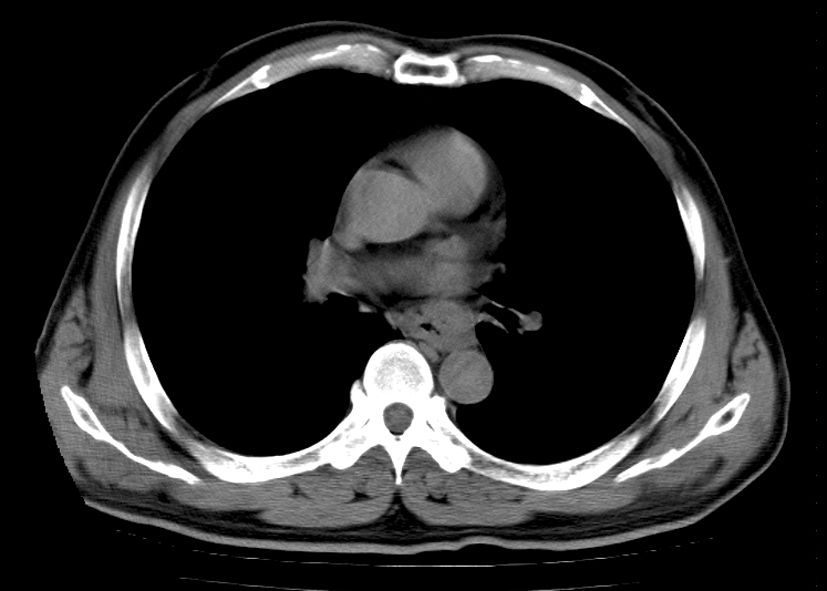
\includegraphics[width=.7\textwidth,height=\textheight,keepaspectratio]{./images/Image00352.jpg}
 \captionsetup{justification=centering}
 \caption{食管癌\\{\small 食管中段管壁不规则增厚}}
 \label{fig17-1}
  \end{figure} 

2.周围脂肪层的消失、模糊:若病灶上下两个层面食管周围脂肪层存在,而仅病灶层面局限性脂肪层消失是诊断肿瘤外侵的标准之一。

3.气管、支气管受侵:①食管肿块侵入气管或支气管,或使之移位,管腔可受压变扁,也可呈管壁增厚。②正常情况下,因气管后壁无软骨支撑、深吸气时气管后壁不应向内凸,而应变平或外凸。如吸气像时看到肿块突入气管或主支气管后壁则可诊为受侵,但这个标准不适于颈部。③肿块所致食管气管瘘。

4.主动脉受侵:①肿瘤与主动脉接触面<45°一般无侵犯;②接触面>90°大多有侵犯;③接触面介于45°~90°可疑侵犯。

5.心包受侵:如果上下层面可见心包有脂肪间隙存在,而病灶层面没有脂肪间隙,则可认为有心包受侵;如所有层面无脂肪间隙则应慎重。如出现心包增厚或结节有特异性。

6.淋巴转移和血行转移。

\textbf{【术后并发症】}
食管癌手术主要为食管胃吻合术伴胸腔胃,其术后并发症如下。

1.早期的并发症:①吻合口瘘;②纵隔脓肿;③淋巴或浆液积聚;④胃出口梗阻;⑤胃坏死、出血等。以吻合口瘘多见,表现为迅速增多的胸腔积液(常在左侧)、纵隔积液。术后纵隔脓肿可见局限液性区域,其中可有气体存在。

2.术后后阶段的并发症:①吻合口瘢痕狭窄;②返流性食管炎;③食管气管瘘;④肿瘤复发等。

此外,食管癌放疗术后食管壁因纤维化而稍增厚,周围脂肪层亦消失。

\textbf{【鉴别诊断】}
本病与食管结核鉴别困难,后者分为增殖型和溃疡型,需密切结合临床进行诊断和鉴别诊断。与平滑肌肿瘤也可鉴别困难。

\subsection{食管平滑肌瘤}

食管肿瘤大多数为恶性,良性肿瘤比较少见,平滑肌瘤占食管良性肿瘤的45%~73%。

\textbf{【病理】}
起源于管壁肌肉,无蒂。呈膨胀性生长,质坚实,被以黏膜。肿瘤可向腔内(黏膜下)或腔外突出、或向腔内外突出呈哑铃状生长。有的可环绕管壁之大部分呈马蹄形。肿瘤大小形态不一,多为单发,少数多发。食管中下段多见。

\textbf{【临床表现】}
病程较长,症状多不显著,为胸骨后不适或喉部异物感,偶有吞咽梗阻的症状。

\textbf{【CT表现】}
食管壁偏心性的软组织肿块,密度均匀、边缘光滑、界限清楚,偶见肿瘤内出血及钙化。增强扫描可有均匀强化。当肿块形态不规则、密度不均、中心有坏死时,平滑肌肉瘤可能性较大。

\textbf{【鉴别诊断】}
①其他良性肿瘤:应与纤维瘤、神经纤维瘤、血管瘤等鉴别,但常有困难。②蕈伞型食管癌:两者可不易鉴别,但食管癌形态不规则,表面常有浅表溃疡、局部食管外脂肪浸润等有助于鉴别。

\subsection{食管破裂}

本病是一种危及生命的急症,能迅速引起暴发性纵隔炎及败血症。

\textbf{【病因】}
①特发性:70%见于剧烈呕吐后,也可见于分娩、排便或痉挛发作时;②肿瘤:如食管癌、肺癌侵及食管;③医源性:如食管破裂修补术后、贲门失弛缓症球囊扩张术后;④外伤性破裂等。

\textbf{【临床表现】} 本病的典型表现是呕吐、胸骨后痛和皮下气肿。

\textbf{【CT表现】}
①局部食管壁增厚:有时由于周围有液体包围而显示不清。②食管腔外气体:是最重要的征象,有时可见颈部及胸部皮下气肿。③胸腔积液:多为双侧,但左侧占优势。可伴有气胸及纵隔内积液。④心包积液及心包增厚。⑤恶性肿瘤还可见纵隔淋巴结增大。

\subsection{食管瘘}

成人的食管瘘多是继发性的改变,常见于肿瘤、创伤所致的感染、食管手术后和放疗、化疗等。CT可发现瘘道并可观察继发的纵隔、肺、心包、膈下的受累情况。

1.食管-气管支气管瘘:由于气管内的气体可自由进入食管,可显示瘘道的准确位置和范围。肺部常伴有吸入性肺炎、肺脓肿等表现。必要时口服造影剂可显示瘘道。

2.食管胸膜瘘:大多可见胸腔积液和气胸,还可见到食管壁的增厚、肺炎、肺不张等。通过口服造影剂可显示穿孔的位置。

3.食管心包瘘:最常见的原因是溃疡和食管炎,其次为恶性肿瘤。CT可见心包内积气积液、心包膜的增厚、心包脂肪层的消失、纵隔积气等。口服造影剂可显示瘘道的位置。

\subsection{贲门失弛缓症}

本病是一种食管肌肉功能紊乱性疾病。

\textbf{【病理】}
因食管下端和贲门丧失正常弛缓功能,食物不能通过食管下端,引起上方的食管扩张、增宽、延长扭曲,食管的肌层可有增厚。后期因管腔高度扩张、管壁相对变薄,可引起穿孔及纵隔炎等。

\textbf{【临床表现】}
发病缓慢,病程较长。主要表现为胸骨后沉重的阻塞感,吞咽困难,在精神紧张时症状可以加重。可出现呕吐,甚至不能弯腰。

\textbf{【CT表现】}
CT扫描关键在于观察是否存在其他疾病或肿瘤。其表现为:食管中度或明显扩张,其内含有气体和液体,管腔在隆突水平的平均直径约4~5cm。管壁无增厚。显著扩张的食管在食管胃连接处变窄,而管壁光滑。

本病与食管癌的发生有相关性,CT可显示癌肿的存在和范围。本病很少发生食管裂孔疝。

\subsection{食管静脉曲张}

CT不是食管静脉曲张的首选检查方法,但它在评价门静脉高压侧支循环的存在和范围上仍是重要的。增强扫描可检出大部分食管静脉曲张。

\textbf{【病理】}
正常情况下,食管下半段的静脉网与门静脉系统的胃冠状静脉、胃短静脉之间存在吻合。当门静脉受阻时,来自消化器官的静脉血不能进入肝内,大量血液通过胃冠状静脉和胃短静脉进入食管黏膜下静脉和食管周围静脉丛,再经奇静脉进入上腔静脉,于是形成食管和胃底静脉曲张。

\textbf{【临床表现】}
食管黏膜因静脉曲张而变薄,易被粗糙食物损伤或黏膜面发生溃疡、糜烂而破裂,导致呕血或柏油样大便。大多门静脉高压所致者可伴脾大、脾功能亢进、肝功能异常及腹水等表现。严重出血者致休克甚至死亡。

\textbf{【CT表现】}
食管和胃壁增厚,食管壁外缘轮廓呈轻度分叶状,扇形的食管腔和向腔内突出的软组织肿块等,须注意结合其他表现与肿瘤鉴别(图\ref{fig17-2})。增强扫描有利于显示食管壁内或胃底壁内的曲张静脉,可呈蚯蚓状或圆形分叶状。同时可见广泛的脾静脉曲张等侧支循环形成和肝脏病变等。

\begin{figure}[!htbp]
 \centering
 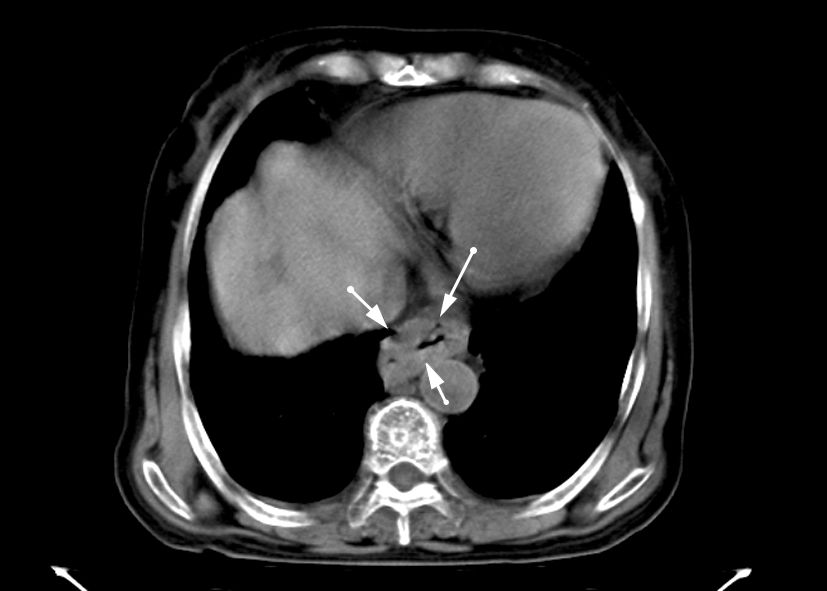
\includegraphics[width=.7\textwidth,height=\textheight,keepaspectratio]{./images/Image00353.jpg}
 \captionsetup{justification=centering}
 \caption{食管静脉曲张\\{\small 食管下端管壁显著增厚,边缘近分叶状}}
 \label{fig17-2}
  \end{figure} 

\subsection{食管裂孔疝}

\textbf{【病因病理】}
可分为先天性和后天性。前者主要指先天性短食管。后天性的发病因素主要有:①膈食管膜松弛;②食管裂孔扩大;③食管绝对或相对变短;④腹内压增大;⑤食管胃角增大变钝(常因胃大部切除所致)。

本病通常分为4型:①先天性短食管型;②牵引型:因炎性挛缩或瘢痕牵引而变短;③食管旁型:疝入胸腔的胃依附着食管下端并与之平行,贲门管与胃的交界点仍然位于膈下;④滑动型:此型最常见。

\textbf{【临床表现】}
轻者无症状,重者有上腹部不适、饱胀、呃气、泛酸和呕吐等。如局部有炎症(返流性食管炎)或溃疡则出现胸骨后烧灼痛。

\textbf{【CT表现】}
正常人的食管裂孔宽2.5cm,食管前庭与胃之间的食管远端为一狭窄段。当有裂孔疝时,此狭窄段消失,被增宽膨大的疝囊所占据(图\ref{fig17-3})。食管远端可见扩张,管腔内有液-气平面,通过口服造影剂可与食管肿块相鉴别。腹部“食管”扩张或中心腱上方出现胃组织,都表明有食管裂孔疝的存在。

\begin{figure}[!htbp]
 \centering
 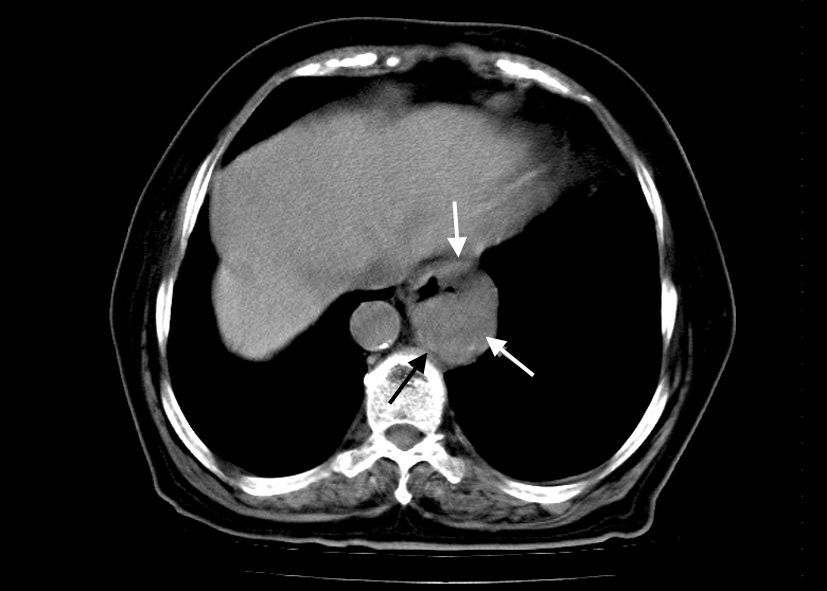
\includegraphics[width=.7\textwidth,height=\textheight,keepaspectratio]{./images/Image00354.jpg}
 \captionsetup{justification=centering}
 \caption{食管裂孔疝\\{\small 膈上可见疝囊,边缘光整}}
 \label{fig17-3}
  \end{figure} 

\section{胃疾病}

\subsection{胃癌}

\textbf{【病理】}
胃癌的病理组织学分为4类:①腺癌;②黏液癌;③低分化癌;④未分化癌。

1.早期胃癌

癌变如仅限于黏膜层或黏膜下层而尚未浸润到肌层者,称为早期胃癌。目前国内外采用日本内窥镜学会所提供的早期胃癌分型:

Ⅰ型:为隆起型早癌。肿瘤突向胃腔,高度超过5mm,呈圆形或类圆形,边界清楚、宽基底、表面毛糙。

Ⅱ型:为表浅或平坦早癌。肿瘤沿黏膜和黏膜下层生长,分界不清,形状不规则。又分为3个亚型:Ⅱa:即表浅隆起型,隆起轻微,不超过5mm;Ⅱb:表浅平坦型;Ⅱc:即表浅凹陷型,凹陷轻微,不超过5mm。

Ⅲ型:为凹陷型早癌。肿瘤发生溃疡,深度在5mm以上,界限清楚,形状不一。

上述几型中凡同时存在两种以上者称为混合型。

2.进展期胃癌

中、晚期胃癌总称为进展型胃癌。国内分为4型:①增生型:亦称蕈伞型、息肉型、肿块型等;②浸润型:亦称硬性癌;③溃疡型;④混合型。

Borrmann分型:Ⅰ型:隆起型,无明显溃疡,为孤立的息肉状癌,以团块状或巢状生长为主;Ⅱ型:局限溃疡型,有环堤和境界鲜明的溃疡形成;Ⅲ型:弥漫溃疡型,亦称浸润溃疡型,以弥漫性生长方式为主;Ⅳ型:弥漫浸润型;Ⅴ型:代表一种未分化类型,即类似于Ⅱc型早期胃癌的进展期胃癌。Ⅱ、Ⅲ型相当于我国的溃疡型。

\textbf{【临床表现】}
早期胃癌症状轻微,多与胃炎和溃疡类似,也可无任何症状。进展期胃癌主要症状为上腹痛、消瘦与食欲减退,呈渐进性加重,贫血与恶病质,还可有恶心、呕咖啡样物或黑便,出现转移后有相应的症状和体征。

\textbf{【CT表现】}

1.CT诊断标准:局部胃壁增厚>5mm,并伴有多层结构的消失或(和)显著异常强化。关于胃癌的强化程度以正常胃壁的强化为标准,当胃壁出现多层强化时,强化程度则以内层的黏膜层为标准。国外有学者认为淋巴结转移的标准是:淋巴结<10mm伴有显著强化或者>9mm;其强化CT值>100Hu;短长轴之比>0.7者为转移。

2.早期胃癌:对于早期胃癌的诊断目前仍有一定争议,大多认为不易检出。①在胃壁多层强化模式中,对于早期胃癌的典型SCT表现,较为公认的看法是显著强化或(和)增厚的内层高密度层,伴有完整的代表黏膜下层的外层低密度带存在。②在胃壁单层强化模式中,早期胃癌特异性表现为仅有显著强化而无胃壁增厚;非特异性表现有胃壁的增厚而不伴有显著强化,此表现多可出现在早期进展期胃癌中。

此外,还可见两种不典型强化表现:①内层高密度黏膜层的局部中断,不伴有异常外层强化。其病理基础为表浅凹陷型和(或)凹陷型早期胃癌伴有完整增厚的低密度黏膜下层。②内层高密度层的局限性息肉状隆起,可同正常黏膜皱襞分开,伴有异常低密度外层增厚。其病理基础为不同程度的反应性黏膜下层纤维化和肌肉增生,轻微凹陷或不规则内表面则代表Ⅱc病变。

3.进展期胃癌:Borrmann分型的各型SCT表现。Ⅰ型:表现为一腔内隆起的肿块;Ⅱ型:增厚的胃壁内见一溃疡存在,且与正常胃壁分界清楚;Ⅲ型:溃疡周边弥漫增厚的胃壁与正常胃壁分界欠清;Ⅳ型:胃壁不规则增厚,胃腔不规则狭窄(图\ref{fig17-4})。轴位图像结合多平面重建(MPR)、三维成像(包括MIP、VR、SSD)及CTVE,可以提高对病变的显示并有利于Ⅱ、Ⅲ型的区分。

\begin{figure}[!htbp]
 \centering
 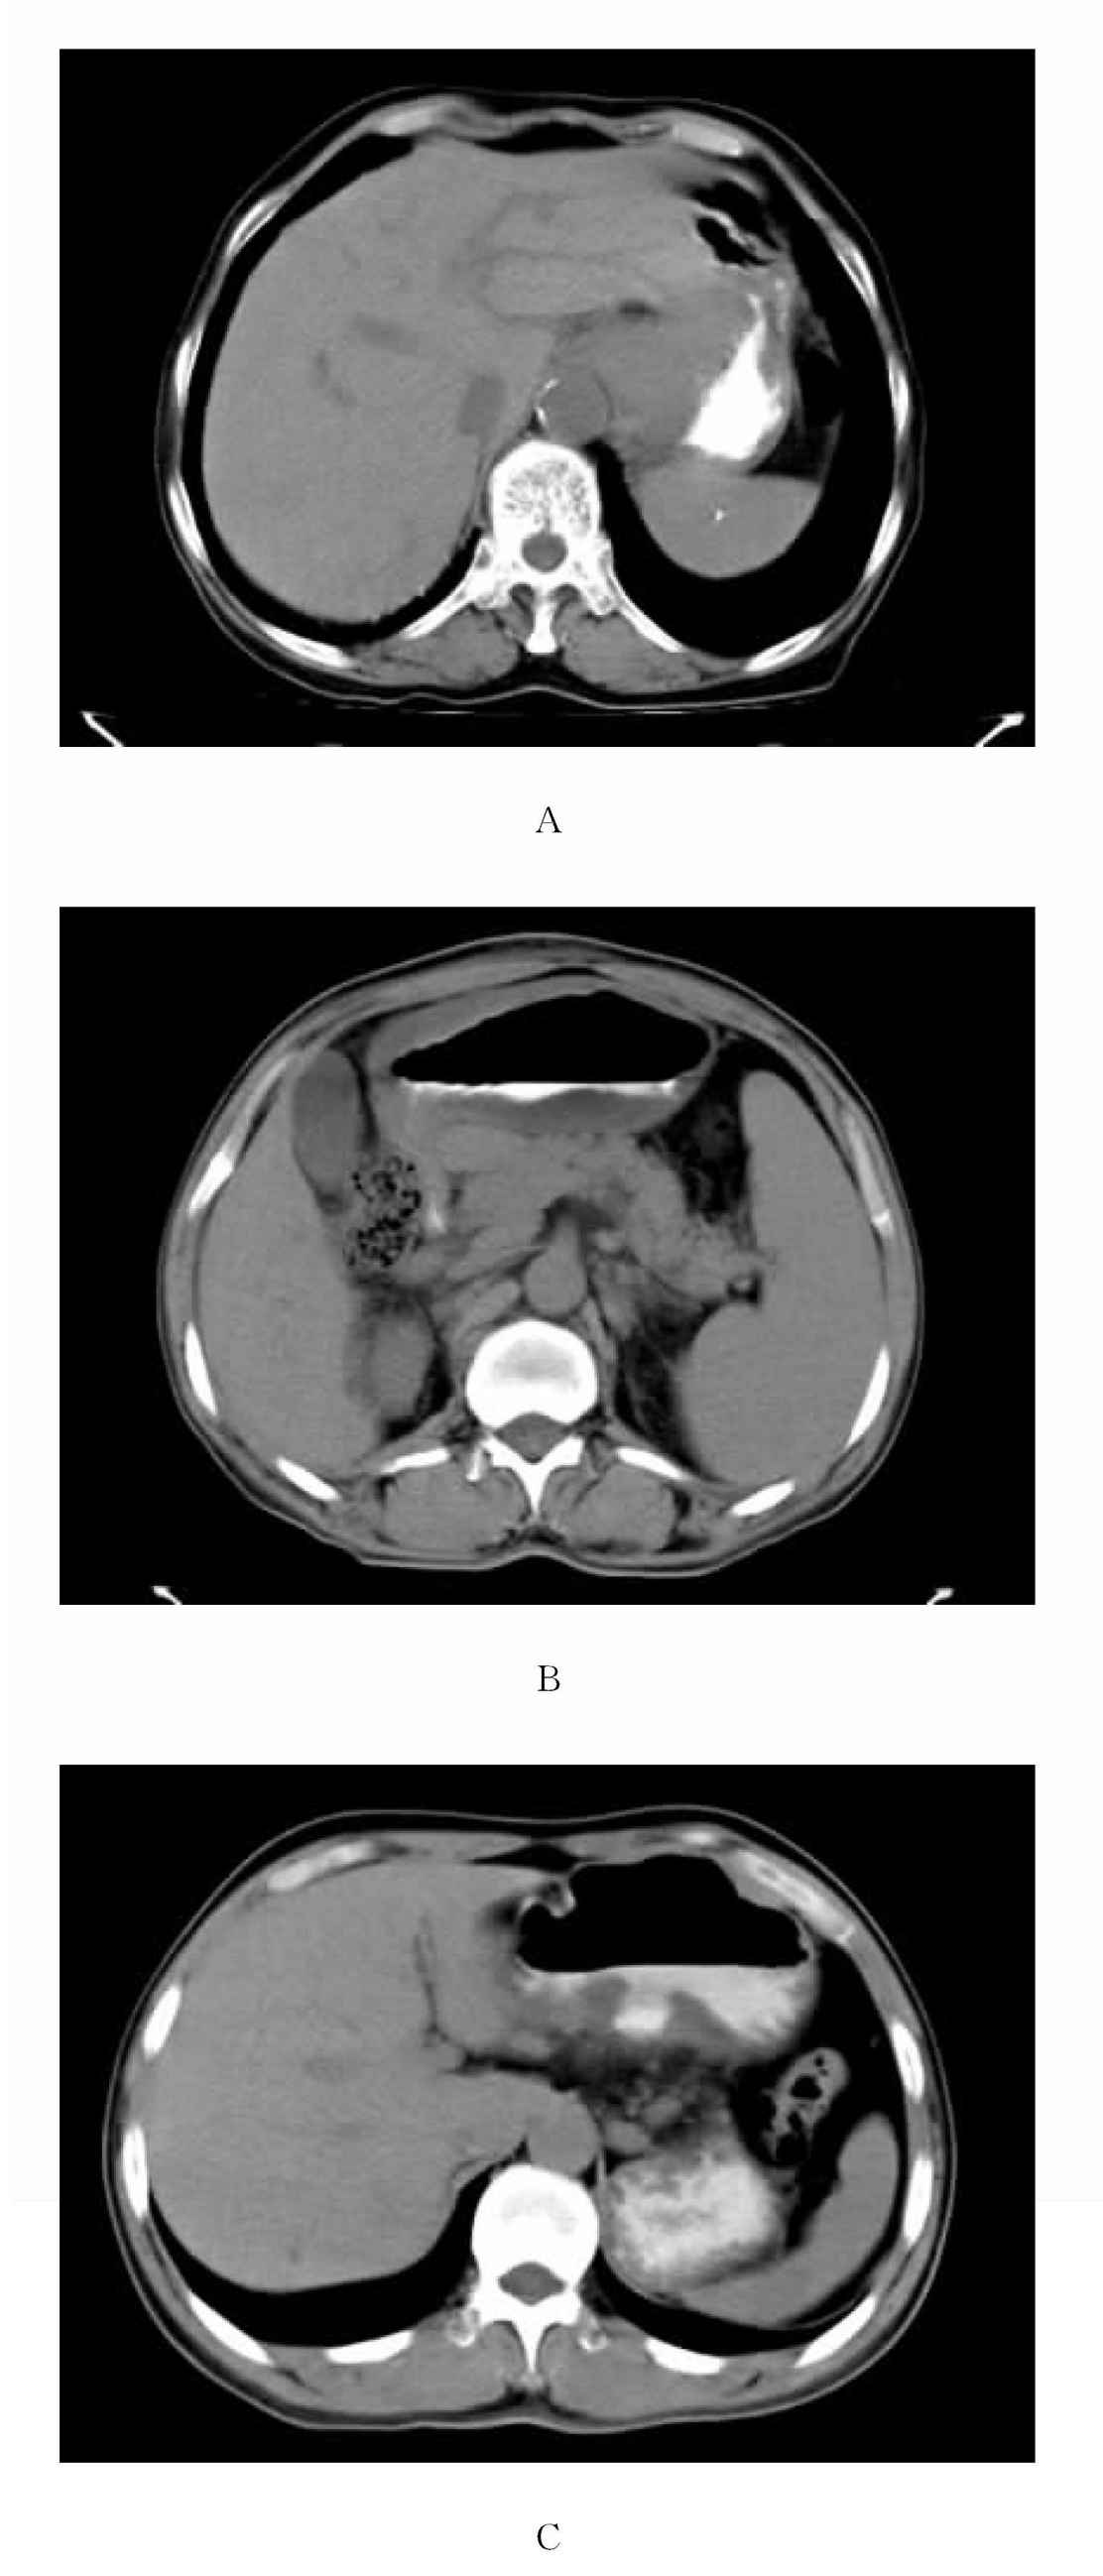
\includegraphics[width=.7\textwidth,height=\textheight,keepaspectratio]{./images/Image00355.jpg}
 \captionsetup{justification=centering}
 \caption{胃癌\\{\small A.贲门癌:贲门区有明显软组织肿块;B.胃窦癌:胃窦壁显著增厚;C.胃体癌:胃体小弯侧胃壁增厚,并可见充盈造影剂的腔内龛影(溃疡)}}
 \label{fig17-4}
  \end{figure} 

国内有学者认为,增强扫描从动脉期(注射造影剂后20~25s)、非平衡期(70~80s,相当于门静脉期)到平衡期(180~240s),肿瘤表现的总趋势是肿瘤从腔内面开始向浆膜面逐渐强化,最终绝大多数肿瘤至平衡期达到均匀强化。

此外,应注意:①胃周脂肪线消失提示已突破胃壁,但并非一定说明癌肿已侵及邻近器官,且脂肪层的变化亦见于炎症;②胃壁增厚还可见于胃淋巴瘤、慢性肥厚性胃炎、胰腺炎和结肠癌侵及胃壁,以及溃疡病等。

\subsection{胃肠道黏膜相关淋巴组织(MALT)淋巴瘤}

本病是一种特殊类型的胃肠道淋巴瘤,属非何杰金淋巴瘤中的外周B淋巴细胞瘤。国外有学者报道,MALT淋巴瘤占原发性胃淋巴瘤的50%~72%。MALT淋巴瘤亦可见于肺、乳房、膀胱、眼结膜、肾、肝、皮肤、唾液腺、甲状腺等。

\textbf{【临床及影像学特征】}
①年龄在50岁以上,多为Ⅰ、Ⅱ期低度恶性肿瘤,病程长、进展缓慢,症状轻、疗效好;②绝大多数幽门螺杆菌阳性,特别是胃MALT淋巴瘤;③消化道钡透示胃小区不规则增宽、多发性黏膜下小结节和多发边缘模糊的浅表溃疡;胃肠道黏膜皱襞粗大、紊乱迂曲;晚期呈多发息肉状结节、肿块及较大溃疡。④CT及MR示胃肠道壁环形光滑或小结节样增厚,肠MALT淋巴瘤可致肠腔狭窄。

总之,多发细小黏膜下病灶及多种征象共存是该病最重要的影像学特点。

\subsection{胃恶性淋巴瘤}

胃淋巴瘤占胃肠道淋巴瘤的50%,其次为小肠、结肠及肠系膜。25%的结外淋巴瘤发生于胃。胃淋巴瘤占胃恶性肿瘤的2%~5%。

\textbf{【病理】}
起源于胃(肠)黏膜固有层和黏膜下层的淋巴组织;2/3以上为非何杰金淋巴瘤(NHL),且绝大多数来自B淋巴细胞(70%),小部分来自T淋巴细胞(25%),极少数来自组织细胞或其他网状细胞(3%~5%);有原发性(>50%)和继发性之分。可分为低分化、中等分化和高分化。大体病理形态有4型:①浸润型:其中霍奇金病(HD)常出现皮革胃样改变;②溃疡型;③息肉型(腔内);④结节型(黏膜下)。

\textbf{【临床表现】}
本病较胃癌的发病年龄小,平均为43.2岁,男性多于女性。上腹痛为最常见的症状,无规律性、制酸剂不能缓解,体重减轻、呕吐或黑便也较常见。偶可表现为自发性胃穿孔症状;而继发性可出现发热、体重减轻、肝脾肿大等全身症状。因早期症状不明显,通常病程较长。

\textbf{【CT表现】} 根据胃侵犯的范围,其CT表现可分为3型。

1.弥漫浸润型:占80%以上。胃壁广泛增厚,其浸润长度超过全胃的1/2。胃壁平均厚度>2cm,最厚可达8cm(图\ref{fig17-5});胃壁外缘呈明显的分叶状或大波浪状,胃腔变形,壁的内缘呈明显的不规则状;在胃充盈程度不同时,胃腔大小尚见有变化,说明胃壁尚有一定柔软度;少数高度肥厚的胃壁内可出现低密度区。增强扫描强化多较均匀、明显,强化幅度较胃癌低10~20Hu。

\begin{figure}[!htbp]
 \centering
 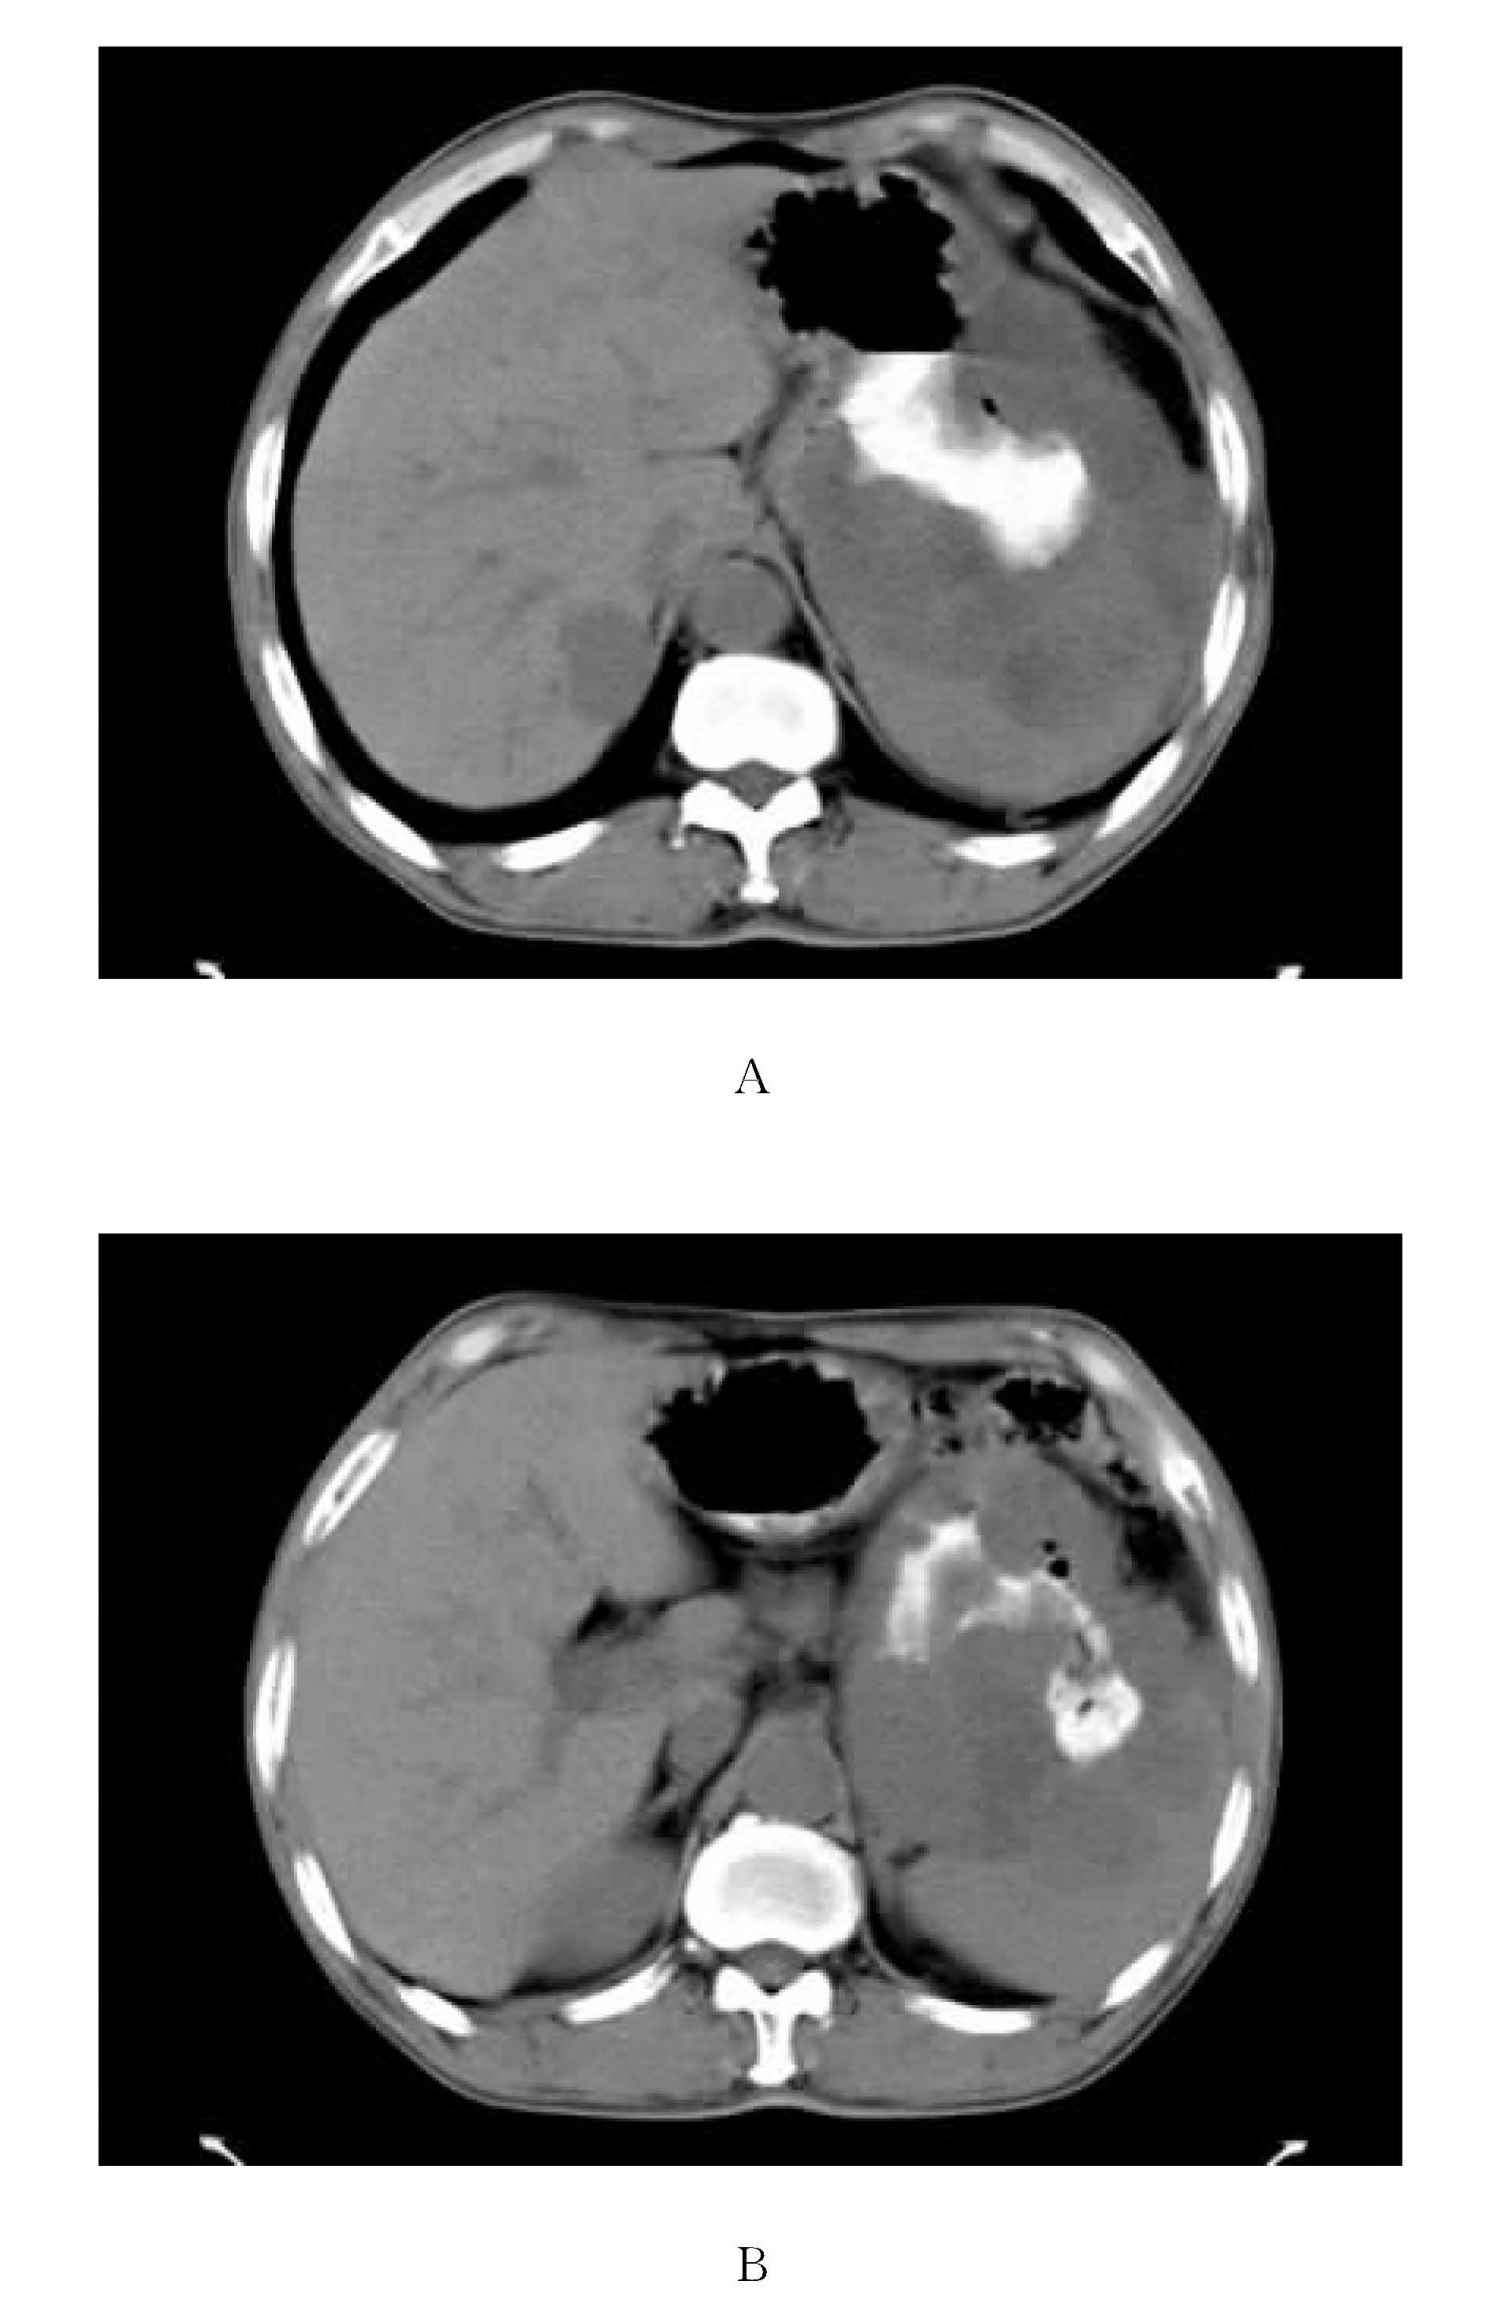
\includegraphics[width=.7\textwidth,height=\textheight,keepaspectratio]{./images/Image00356.jpg}
 \captionsetup{justification=centering}
 \caption{胃恶性淋巴瘤\\{\small 胃底、体部胃壁广泛增厚,最厚处约7cm,侵犯胃周径3/4以上;边缘较光滑、清楚,胃周脂肪层仍存在;脾脏受压,界限不清}}
 \label{fig17-5}
  \end{figure} 

2.节段型:胃壁广泛增厚,侵及胃的范围小于胃长度的1/2。

3.局灶型或息肉型:胃局灶性增厚或突向腔内的息肉样肿块,强化也较均匀、明显。少数表现为溃疡型肿块,但淋巴瘤的溃疡浅而大。

总之,胃淋巴瘤病灶边缘较光滑、清楚,胃周脂肪层仍存在。胃壁广泛增厚或巨大的胃肿块而邻近无侵犯或侵犯不明显是其特点。有人认为胃壁厚度≥4cm,侵犯胃周径50%以上淋巴瘤可能性达83%,胃癌仅占9%。此外,胃淋巴瘤胃底、体常同时受累。

\textbf{【鉴别诊断】}
与胃癌的鉴别有时较困难,下列几点有助于鉴别:①胃淋巴瘤时,胃壁平均厚度(4~5cm)较胃癌(2cm)大;②胃淋巴瘤的胃壁浸润虽厚,其柔软度常不一致;而浸润性癌则多见胃壁僵直;③有学者认为淋巴瘤胃(肠)壁的淋巴细胞增殖没有破坏正常细胞,因而无成纤维反应,故胃(肠)腔缩小或梗阻相对胃(肠)癌少见;④当病变外侵和(或)有腹腔淋巴结肿大时,胃癌可能性较淋巴瘤大;而淋巴瘤胃周脂肪消失与邻近脏器侵犯不及胃癌常见;⑤当病变厚度>4cm,且侵犯周径50%以上时淋巴瘤可能性较胃癌大,而且淋巴瘤常累及多个部位,胃底、体同时受累最常见;⑥增强扫描胃淋巴瘤强化不及胃癌;⑦国外有学者认为不伴有胃周淋巴结增大的肾门水平以下腹膜后淋巴结增大为淋巴瘤的特点。

\subsection{胃平滑肌源性肿瘤}

胃是胃肠道平滑肌源性肿瘤最多发生的部位,是胃的非上皮性肿瘤中最常见的。包括良性的平滑肌瘤和恶性的平滑肌肉瘤,以及虽属良性但可有淋巴和肝转移的平滑肌母细胞瘤。

\textbf{【病理】}
胃平滑肌源性肿瘤的病变部位以胃体部多见占58%,胃底19%,胃窦11%,贲门部11%,底体交界和体窦交界处各占1%。多单发、偶多发。大体病理可分为腔内型、腔外型和腔内外型。镜下平滑肌瘤无核分裂、异形性不明显;平滑肌肉瘤则有不用程度的核分裂、异形性明显,如核的多形性、核大而浓染。平滑肌瘤约2.1%发生肉瘤变。

\textbf{【临床表现】}
本病以中老年多见,男女之比为2∶1。症状无特异性,上腹部疼痛、呕血、黑便是常见的症状。

\textbf{【CT表现】} 胃平滑肌瘤和平滑肌肉瘤CT表现基本一致。

1.平滑肌瘤:多为圆形或椭圆形软组织肿块,与胃壁广基或带蒂相连。直径多<5cm。除少数有散在钙化或中央呈低密度外,多密度均匀,强化均一。

2.平滑肌肉瘤:呈椭圆形或不规则分叶状肿块,宽基底与胃壁相连。直径多>5cm。肿块内有明显坏死液化区,增强后密度不均匀;黏膜面有大小不等的溃疡(图\ref{fig17-6})。肿瘤还可直接侵及邻近脏器或出现远处肝转移等。此外,胃内型和胃壁型者部分可有与胃腔相通的窦道形成;胃外型者亦常有大的溃疡并与胃腔相通;肿块巨大者可致定位困难。

总之,除直接浸润和远处转移提示为恶性外,肿瘤大、分叶状、不均匀强化及溃疡形成均提示平滑肌肉瘤可能性大。

\begin{figure}[!htbp]
 \centering
 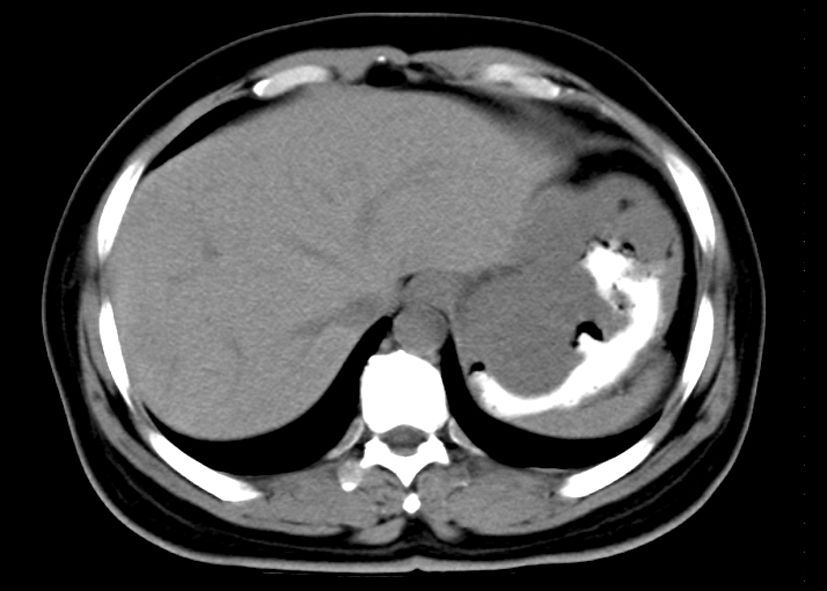
\includegraphics[width=.7\textwidth,height=\textheight,keepaspectratio]{./images/Image00357.jpg}
 \captionsetup{justification=centering}
 \caption{胃底平滑肌肉瘤\\{\small 胃底有巨大软组织肿块,其表面可见多个不规则溃疡并伸入瘤体内形成坏死腔,腔内充有高密度造影剂和气体}}
 \label{fig17-6}
  \end{figure} 

\subsection{胃肠道间质瘤}

胃肠道间质瘤以往归为平滑肌肿瘤。有学者提出广义的胃肠道间质瘤包括发生于胃肠道平滑肌细胞来源的肿瘤、神经鞘细胞来源的肿瘤、平滑肌和神经鞘细胞双向分化的肿瘤,以及未定分化的肿瘤。随着病理学的发展,尤其是免疫组化和超微结构的研究进展,现多认为是一类独立的、来源于胃肠道原始间叶组织的非定向分化的肿瘤,部分可伴有平滑肌和(或)神经鞘细胞的不完全分化,即狭义的胃肠道间质瘤。国外文献统计,本病是最常见的胃肠道间叶性肿瘤(约占全部胃肠道间叶性肿瘤的80%,但远少于上皮性肿瘤和淋巴瘤),占全部胃肠道肿瘤的1%~3%;而平滑肌瘤和平滑肌肉瘤较为罕见。

\textbf{【病理】}
本病发生于胃肠道固有肌层,目前认为细胞起源为正常成人胃肠道的肠肌神经丛Cajal间质细胞。本病以胃部常见,约占60%~70%,其次为小肠约20%~30%,直肠5%~15%,食管和结肠仅5%。由原始的相对未分化的间质细胞增生而成。可分别由编织状排列的长梭形细胞组成的梭形细胞型(70%)和由成团或成片的上皮细胞组成的上皮细胞型(30%)。大多为恶性,可发生血行及淋巴转移,其良恶性尚无统一病理诊断标准。

\textbf{【临床表现】}
本病以中老年男性多见。以反复发作的腹部隐痛为主要症状,可有慢性消化道少量出血,腹部肿块出现较迟。少数无症状而偶然发现。其最主要的特征是免疫组织化学表达KIT(CD117)几乎均为阳性;约70%同时表达CD34阳性。部分也可表达平滑肌肌动蛋白(20%~30%),少数可表达肌间蛋白或S-100蛋白。

\textbf{【影像学表现】}
与平滑肌类肿瘤相似,无特异性。①良性:病灶直径多<5cm,边缘清楚,不侵犯邻近结构,肿块很少坏死。增强扫描多轻度均匀强化。②恶性:病灶直径多>5cm,边缘常不清楚,多容易侵犯邻近组织器官甚至远处转移,病灶中央常见缺血坏死形成的低密度区(图\ref{fig17-7}),病灶内钙化以恶性者多见。增强扫描实性部分可明显强化。坏死严重者,可与肠腔相通形成气液面,但很少出现肠梗阻征象。

\begin{figure}[!htbp]
 \centering
 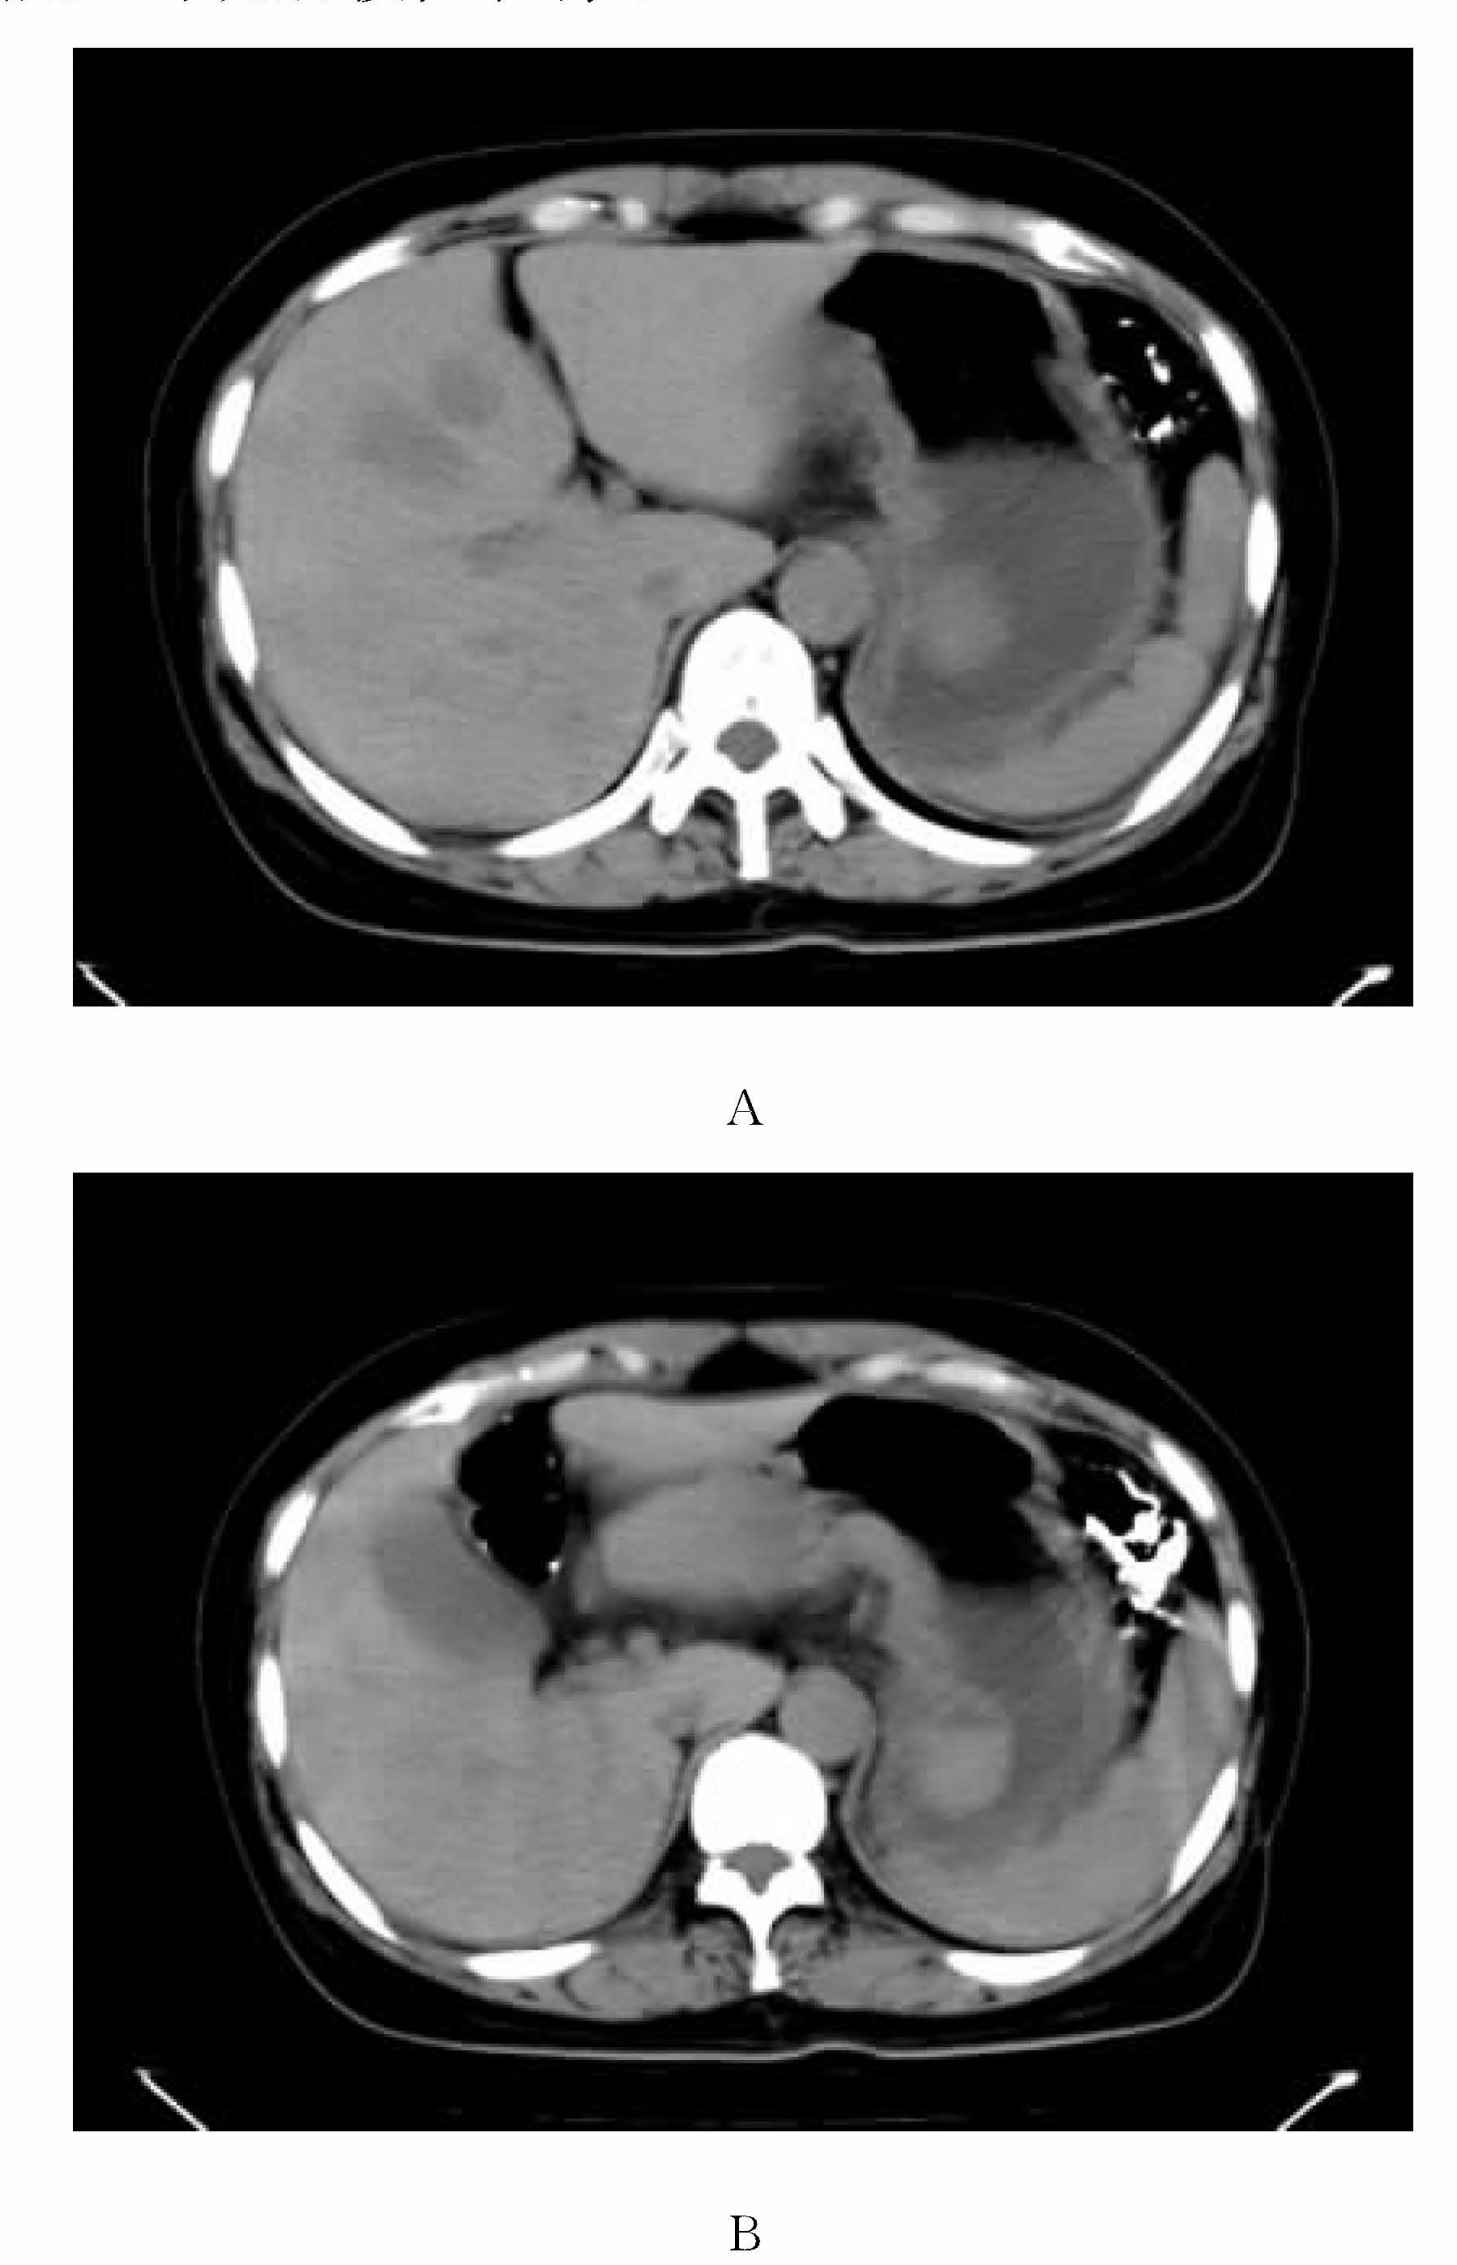
\includegraphics[width=.7\textwidth,height=\textheight,keepaspectratio]{./images/Image00358.jpg}
 \captionsetup{justification=centering}
 \caption{胃间质瘤\\{\small A、B为同一患者的上下连续层面,病理为低度恶性。贲门下方可见高密度灶突向腔内,密度均匀、边缘光滑}}
 \label{fig17-7}
  \end{figure} 

\subsection{胃少见的良性肿瘤}

除平滑肌肿瘤外,胃其他良性肿瘤不多见。有起源于黏膜上皮的胃腺瘤、绒毛状腺瘤,位于黏膜下的脂肪瘤、血管瘤、神经纤维瘤、畸胎瘤等。

\subsubsection{胃腺瘤}

腺瘤性息肉与炎性息肉影像学表现相似,难以区分,两者在CT上偶可见到。

\textbf{【CT表现】}
呈圆形或椭圆形、表面光滑;大小多在1cm左右;带蒂或广基均可,周围胃壁正常。与胃癌不难鉴别,但应注意不可将粗大的黏膜皱襞当作带蒂息肉(图\ref{fig17-8})。

\begin{figure}[!htbp]
 \centering
 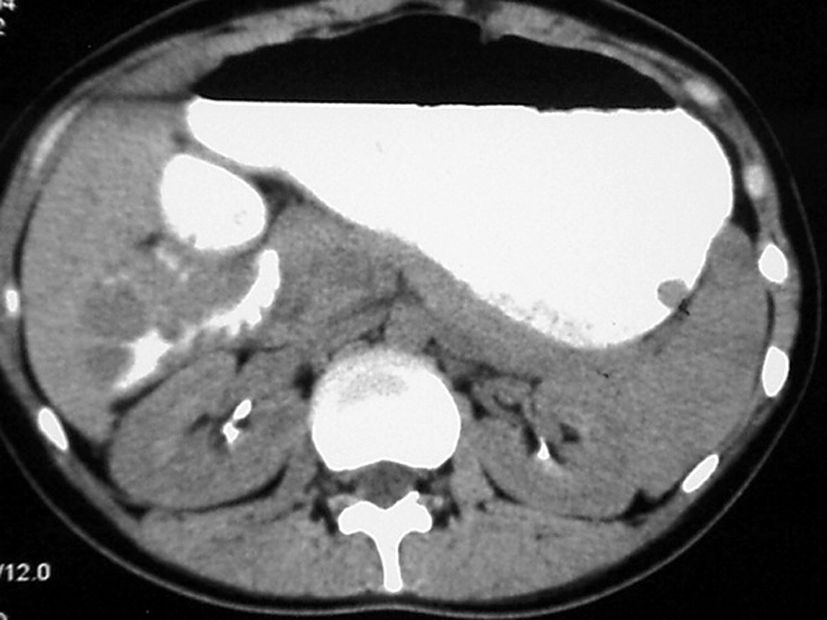
\includegraphics[width=.7\textwidth,height=\textheight,keepaspectratio]{./images/Image00359.jpg}
 \captionsetup{justification=centering}
 \caption{胃腺瘤样息肉\\{\small 胃体部大弯侧有基底较窄的低密度小结节,十二指肠区也有充盈缺损(本病例为胃、肠多发性腺瘤样息肉并发多部位肠套叠)}}
 \label{fig17-8}
  \end{figure} 

\subsubsection{胃绒毛状腺瘤}

又称为乳头状腺瘤。本病有高度恶变危险性,病变越大恶性变可能越大。

\textbf{【CT表现】}
呈广基、不规则分叶状伴许多叶状突起的肿块,可单发或多发;直径为3~9cm大小,大者可达15cm。由于病灶较柔软,故即使病变很大也可无胃肠道梗阻。

\subsubsection{胃脂肪瘤}

由分化良好的脂肪组织被纤维囊包围组成。

\textbf{【CT表现】}
表现为较小的壁内或突向胃腔的圆形或椭圆形肿块,可变形,界限清楚;CT值为-90~-120Hu。大者表面可有糜烂、溃疡。

\subsubsection{胃血管瘤}

目前尚不能确认是真正的肿瘤还是一种先天性畸形。

\textbf{【CT表现】}
平扫表现与其他黏膜下肿瘤极相似,但有时可显示肿瘤内静脉石;增强扫描显著强化(CT值可达100Hu左右)有助于确诊。

\subsubsection{胃神经鞘瘤}

本病极为少见,占胃神经源性肿瘤的78.0%~82.4%,多为良性,恶性较罕见。

\textbf{【CT表现】}
可分为局灶性结节或肿块型、胃壁局限增厚型和局块型;也有文献报道表现为圆形、卵圆形或扁圆形均匀实性肿块。还有文献报道平扫肿瘤密度常略低于周围的肌肉组织(因神经组织内含质量较高),CT值30~50Hu;密度多均匀,强化不明显或轻度强化;但也有文献报道呈缓慢、均匀中度强化。但有时肿瘤较小时就出现明显甚至多发低密度区,是因坏死、囊变、陈旧出血或肿瘤富含Antoni
B细胞区所致,但多为囊变区。

\subsection{胃溃疡}

本病一般不做CT检查,CT主要用于溃疡并发症的检查,在良性鉴别方面也有一定的价值。

\textbf{【病理】}
常单发,多在胃角附近,其次为胃窦部,其他部位比较少见。主要病理改变为胃壁糜烂缺损,形成壁龛。溃疡先从黏膜开始,逐渐侵及黏膜下层,常深达肌层。溃疡多呈圆形或椭圆形。慢性溃疡如深达浆膜层时,称为穿透性溃疡;如浆膜层穿破且穿入游离腹腔者为急性穿孔;也可与网膜、胰腺等粘连,甚至穿入其中则为慢性穿孔。溃疡周围有坚实的结缔组织增生者,称为胼胝性溃疡。溃疡愈合后常有不同程度的瘢痕形成,严重者可导致胃变形,可恶性变。

\textbf{【临床表现】}
以慢性、反复性、周期性和节律性上腹部疼痛为主要表现,其他还有恶心、呕吐、嗳气、返酸等症状。若有出血则有呕血和黑便。严重者可有幽门梗阻。

\textbf{【CT表现】}

1.一般表现:胃壁缺损和胃壁增厚,缺损区多光整。病变区与正常胃壁交界清楚、自然,邻近胃壁轻度增厚。深达浆膜层的溃疡,胃的浆膜层可毛糙,与周围组织和器官之间出现粘连带。

2.穿透性溃疡:胃壁的缺损达浆膜层外,周围有广泛粘连,形成炎性肿块。有时在小网膜囊内见到含气的液平面或对比剂影,周围由软组织或脏器包绕。胃溃疡穿孔可见小网膜囊内积气,胃周围软组织密度肿块。

3.巨大溃疡和胼胝性溃疡:与早期溃疡型胃癌难以鉴别。良性溃疡有以下特点:胃壁的缺损区多光整、对称,局部增厚的胃壁均匀,邻近增厚的胃壁呈明显的对称性且光整是其特点,病变区与正常胃壁交界区逐渐移行、自然。

\subsection{胃黏膜巨大肥厚症}

本病又称巨大肥厚性胃炎、假肿瘤性胃炎、肥厚性胃病、胃巨大皱襞症及Menetrier病等。本病少见,病因不明。

\textbf{【病理】}
以胃黏膜局限性或弥漫性脑回状增大为特征。镜检胃腺体增多、延长、迂曲,其基底有囊样变化,并可伴有轻度炎症细胞浸润和水肿。

\textbf{【临床表现】}
临床症状变化多端,与胃溃疡相似,如腹痛、腹胀、恶心、呕吐、厌食、呕血和黑便,胃酸变化无规律性。可伴有低蛋白血症(由于腺体分泌大量蛋白所致)。

\textbf{【CT表现】}
有以下特点(图\ref{fig17-9}):①黏膜皱襞明显粗大呈指状及息肉状;②皱襞间隙较规则,且间隙区基底部的胃壁厚度基本正常;③胃浆膜面光整;④病变呈弥漫性,以胃体、底部大弯侧明显;⑤胃皱襞厚度随充盈程度而变化,即有可变性。

\begin{figure}[!htbp]
 \centering
 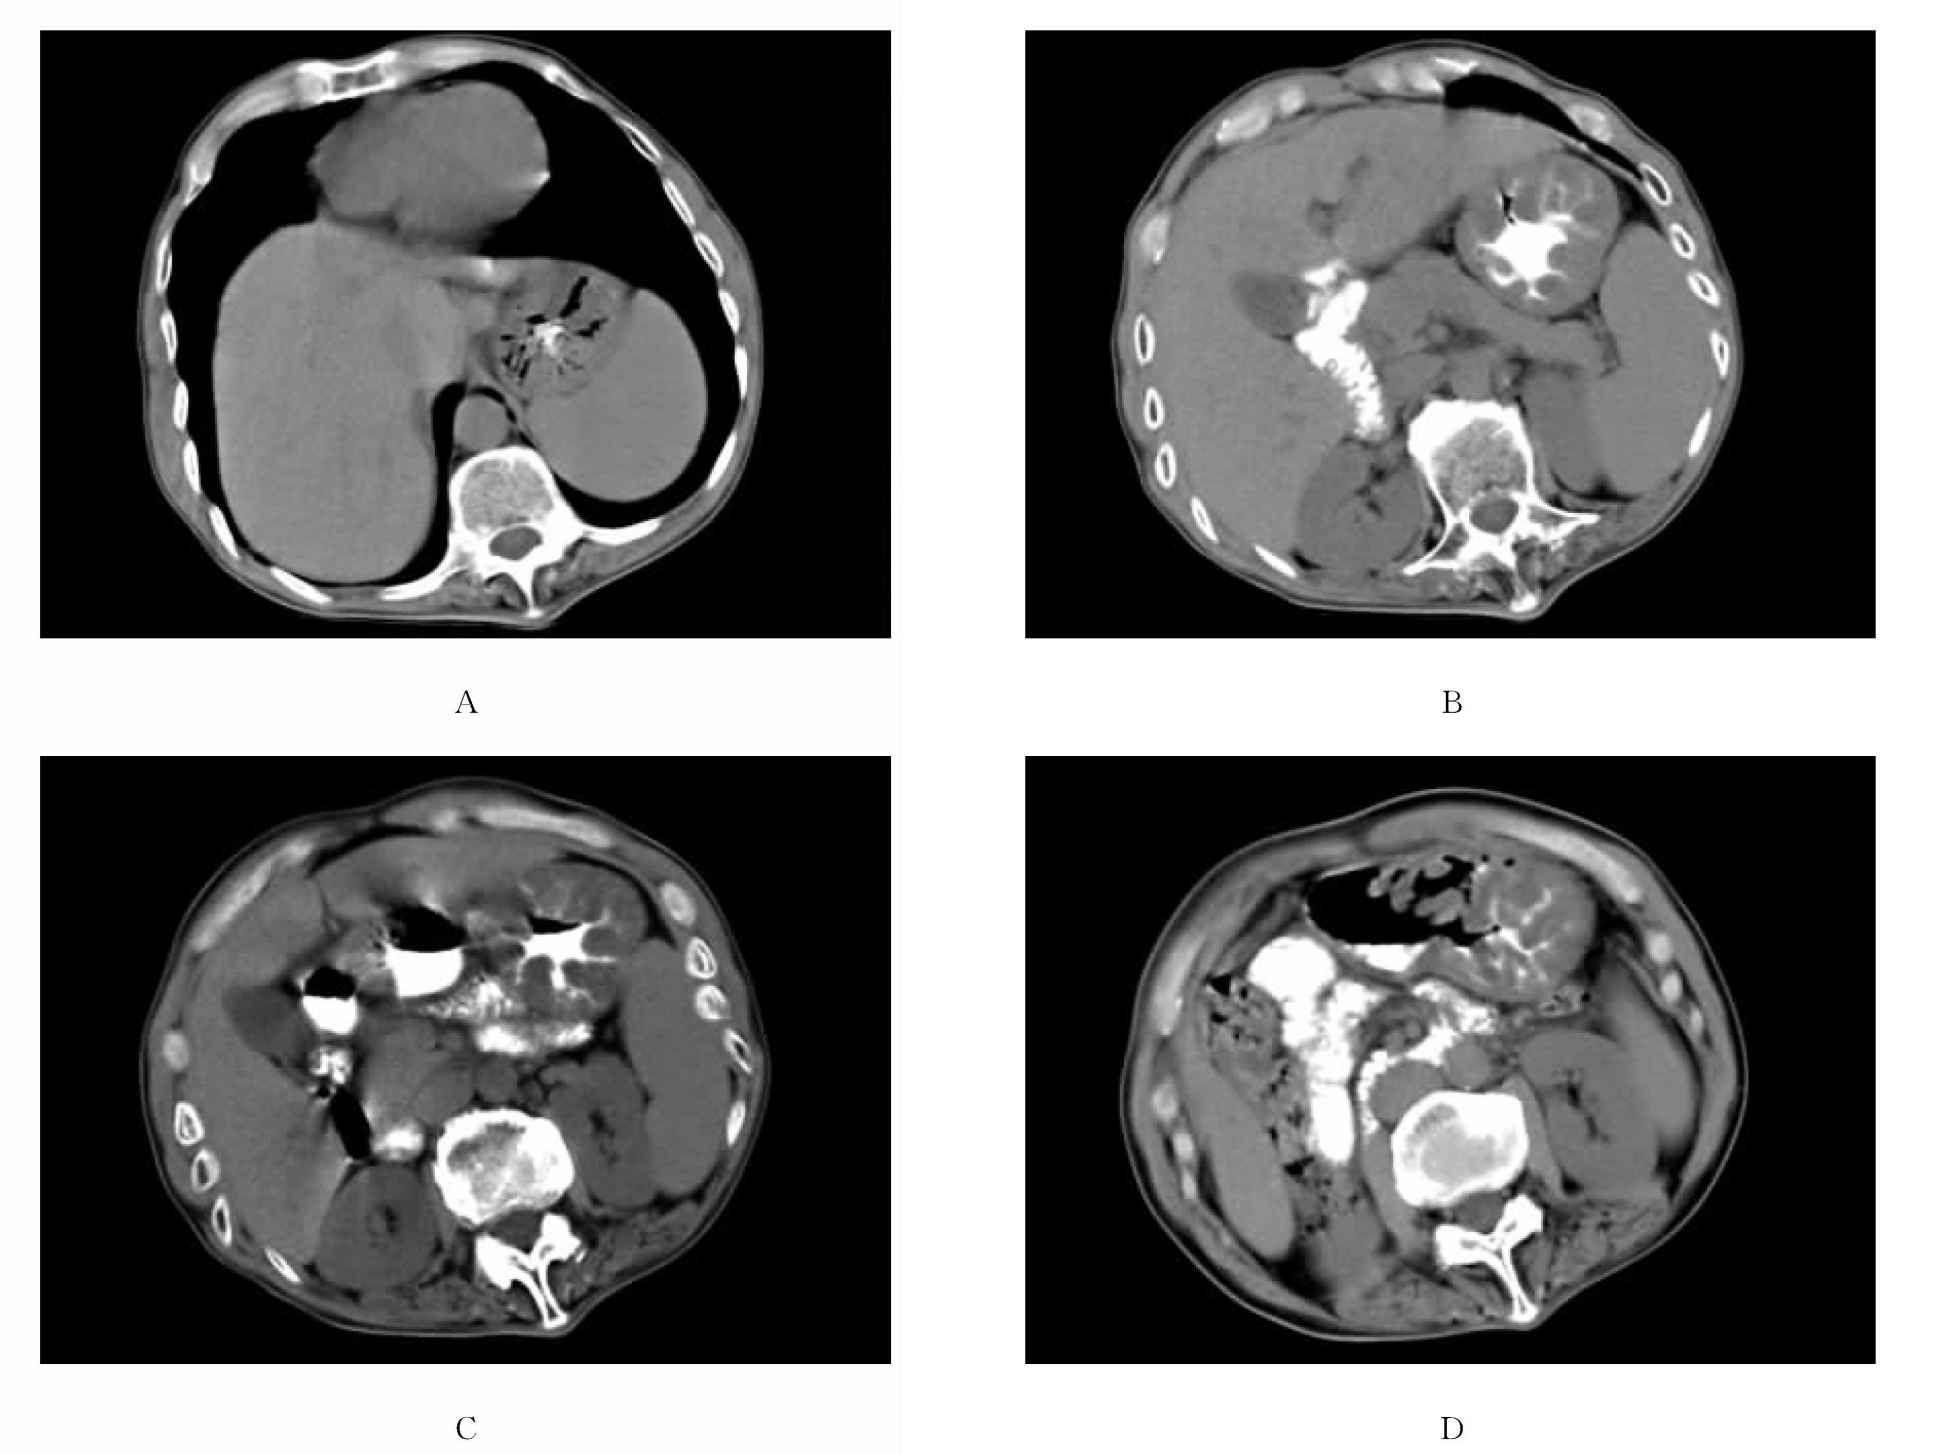
\includegraphics[width=.7\textwidth,height=\textheight,keepaspectratio]{./images/Image00360.jpg}
 \captionsetup{justification=centering}
 \caption{胃黏膜巨大肥厚症\\{\small A~D为同一患者。胃黏膜皱襞明显粗大呈指状;皱襞间隙较规则,间隙区基底部的胃壁厚度正常;胃浆膜面光整;病变以胃体、底部为著}}
 \label{fig17-9}
  \end{figure} 

\subsection{胃憩室}

胃壁局限性向外突出的囊袋状结构称为胃憩室。

\textbf{【病因病理】}
分为先天性及后天性两种:①先天性:多位于胃贲门近小弯侧后壁,是因此处为胃壁生理性薄弱点,肌层薄弱所致。②后天性:多位于幽门附近,常为胃周淋巴结等炎性瘢痕粘连牵引所致。

病理可分为3种类型:①真性憩室:憩室壁具有胃壁各层结构;②假性憩室:憩室壁无肌层参与;③壁内憩室:即胃黏膜面突入胃肌层内,未超过浆膜面,此型十分少见。

\textbf{【临床表现】}
多无症状。有的可有上腹部不适;当有溃疡、出血或穿孔等可有相应症状和体征。

\textbf{【CT表现】}
可显示圆形、椭圆形,呈窄颈(先天性)或宽颈(多为后天性)的囊袋样突出;其内有造影剂或(和)气体充盈。如憩室内无气体或造影剂而显示呈实体时,易误诊为软组织结节或肿块。

\subsection{胃重复畸形}

消化道重复畸形是少见的胚胎发育畸形,可发生于从舌至肝门的任何部位。其病因及发病机理存在着多源性。其发病部位以回肠及回盲部多见,约占50%~70%,其次为大肠、空肠、食管、胃、十二指肠。

\textbf{【病理】}
消化道重复畸形系紧密附着于消化道的球形或管状空腔器官,具有消化道结构,并与主胃(肠)管有着共同的血供。空腔器官(囊)内充有黏液物质,其分泌程度决定了囊的大小,囊腔极少与胃腔相通。

\textbf{【临床表现】}
主要表现为腹部肿块,以及因黏膜分泌的消化液腐蚀囊壁产生消化性溃疡或异位组织中的胰腺炎所引起的症状,包括呕吐、腹痛和消化道出血等。

\textbf{【CT表现】}
显示为一起自胃壁的囊状或管状的低密度肿块。增强扫描其壁可强化。HRCT可显示其胃壁的多层结构特征而做出诊断。注意勿误诊为胰腺假性囊肿。

\section{十二指肠疾病}

\subsection{憩室和炎症}

十二指肠的良性病变主要有良性溃疡、憩室和炎症,CT检查价值不大。

1.十二指肠良性溃疡:CT一般难以显示。但在溃疡发生穿孔时,CT可了解穿孔的范围、邻近脏器的受累情况、有无脓肿或窦道形成等情况。

2.十二指肠憩室:CT表现为肠腔外含有造影剂或气体的小囊腔(图\ref{fig17-10}),薄层扫描可显示其颈部。

\begin{figure}[!htbp]
 \centering
 
\includegraphics[width=.7\textwidth,height=\textheight,keepaspectratio]{./images/Image00361.jpg}
 \captionsetup{justification=centering}
 \caption{十二指肠憩室\\{\small 十二指肠降部内侧有近圆形低密度气囊}}
 \label{fig17-10}
  \end{figure} 

3.十二指肠炎症:CT主要表现为肠壁的广泛性增厚,肠壁密度稍低,但强化均一。有时需与肿瘤性的肠壁增厚鉴别,鉴别的要点为观察增厚的肠管能否扩张。

\subsection{十二指肠良性肿瘤}

\subsubsection{腺瘤}

\textbf{【病理】}
与胃相反,发生于十二指肠的上皮性息肉大多数不是炎性的,而是腺瘤性息肉。此外,发生于黏膜上皮的十二指肠腺瘤中尚有绒毛状腺瘤(较其他腺瘤大,且较发生于结肠者更易恶变)和家族性大肠息肉病(也易恶变)。

\textbf{【临床表现】}
多无症状,仅在钡餐透视时偶然发现。CT检查意义不大,但引起胆胰管阻塞者CT检查有帮助。

\textbf{【CT表现】}
其形态特点为起自上部或降部的单个生长的光滑、无蒂的息肉样病变突向肠腔内,乳头部腺瘤可有胆胰管的阻塞扩张。此外,绒毛状腺瘤呈菜花状,但CT检查可能难以显示其边缘特点。

\subsubsection{间质性良性肿瘤}

\textbf{【病理】}
即发生于黏膜下的间质性良性肿瘤,依次为脂肪瘤、平滑肌瘤、血管瘤和错构瘤。

\textbf{【临床表现】}
肿瘤小者多无明显症状。大者可出现上腹部不适、恶心、呕吐,甚至因肿瘤出血或表面溃疡出血而致黑变。

\textbf{【CT表现】}
①脂肪瘤:位于肠壁的、轮廓境界清楚的脂肪密度肿物,无强化,易确诊。②平滑肌瘤:多表现为直径<3.0cm的圆形、密度均匀的肿块,定性困难。③血管瘤:罕见,其显著强化的特点有助于确诊。

\subsection{十二指肠恶性肿瘤}

对小肠恶性肿瘤来说,上皮性(癌)以十二指肠多见,其次为空肠,回肠最少发病;而间质性(肉瘤)则相反,十二指肠最少见,依次为空肠、回肠发病最多。总之,十二指肠恶性肿瘤最常见者为腺癌,其次为平滑肌肉瘤、恶性淋巴瘤,还有类癌等。

\subsubsection{十二指肠腺癌}

\textbf{【病理】}
十二指肠腺癌是小肠最常见的原发性恶性肿瘤。约40%~50%的小肠腺癌发生于十二指肠,特别是壶腹部或在十二指肠乳头以下的区域。病理上分为息肉(可多发)、溃疡、浸润3型。

\textbf{【临床表现】}
无特异性。早期可无任何症状,也可有腹痛、上腹部不适等。随肿瘤发展可有腹痛加重、呕吐、出血、体重减轻,也可有黄疸、便血等。

\textbf{【CT表现】}
可见腔内息肉状肿块(图\ref{fig17-11}),或肠壁不规则浸润性增厚、肠腔狭窄变形,偶见龛影。肿块多<8cm,肠壁厚多>1cm。强化程度不一。乳头部及邻近者可有胆、胰管的阻塞扩张。CT检查还可了解有无周围组织器官的浸润及远处转移。

\begin{figure}[!htbp]
 \centering
 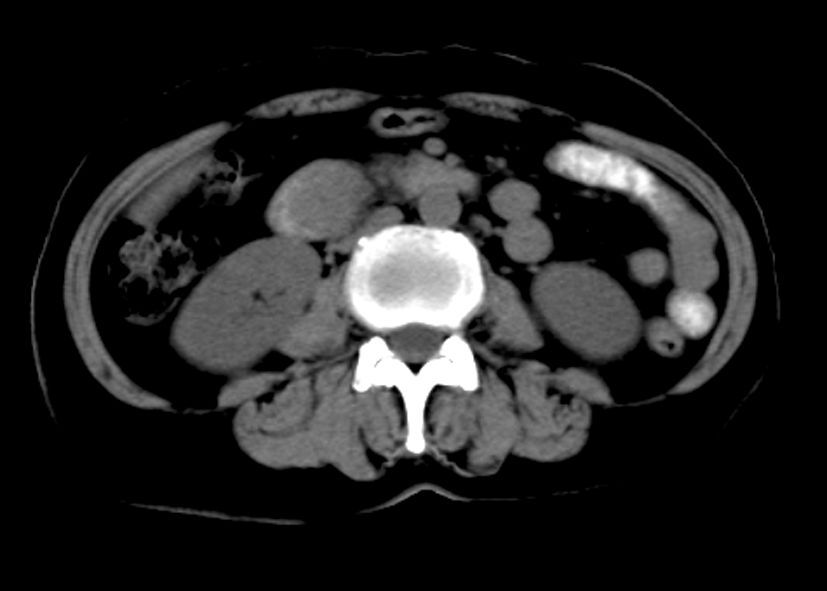
\includegraphics[width=.7\textwidth,height=\textheight,keepaspectratio]{./images/Image00362.jpg}
 \captionsetup{justification=centering}
 \caption{十二指肠乳头癌(手术证实)\\{\small 十二指肠乳头区有软组织密度结节,边缘光滑}}
 \label{fig17-11}
  \end{figure} 

\subsubsection{平滑肌肉瘤}

\textbf{【病理】}
平滑肌肉瘤是十二指肠间质性恶性肿瘤中最常见者。约占全部十二指肠恶性肿瘤的10%,约80%发生于十二指肠的降部和水平部。多单发。肿瘤起自黏膜下层,易形成表面溃疡和坏死腔,故即使肿块很大也很少引起梗阻,而倾向于邻近结构侵犯。

\textbf{【临床表现】}
临床症状出现较晚。可有上腹部不适、腹痛、出血、体重减轻等,梗阻与黄疸少见或较轻,腹部肿块触及率高。

\textbf{【CT表现】}
肿瘤呈突向腔内外的实质性肿块,偶有钙化,并可见其表面溃疡。增强扫描富血供者强化明显,而少血管性者则强化稍差;中心坏死区呈低密度不强化灶,并可见肿块内液-气平面或厚壁空洞。晚期常转移至肝、网膜及腹膜。

\textbf{【鉴别诊断】}
十二指肠原发恶性肿瘤应注意与邻近恶性肿瘤的直接侵犯相鉴别。主要见于胰腺癌、淋巴瘤、周围淋巴结转移瘤,还可见于结肠癌、肾细胞癌、胆囊癌等。此外,腺肌增生症为十二指肠上皮陷入肌层内生长所致,是一种非炎性、非肿瘤性的变性腺体增生性疾患,临床上少见,鉴别困难。

\section{小肠疾病}

\subsection{概述}

\subsubsection{}

\begin{table}[htbp]
\centering
\caption{小肠非肿瘤性疾病}
\label{tab17-1}
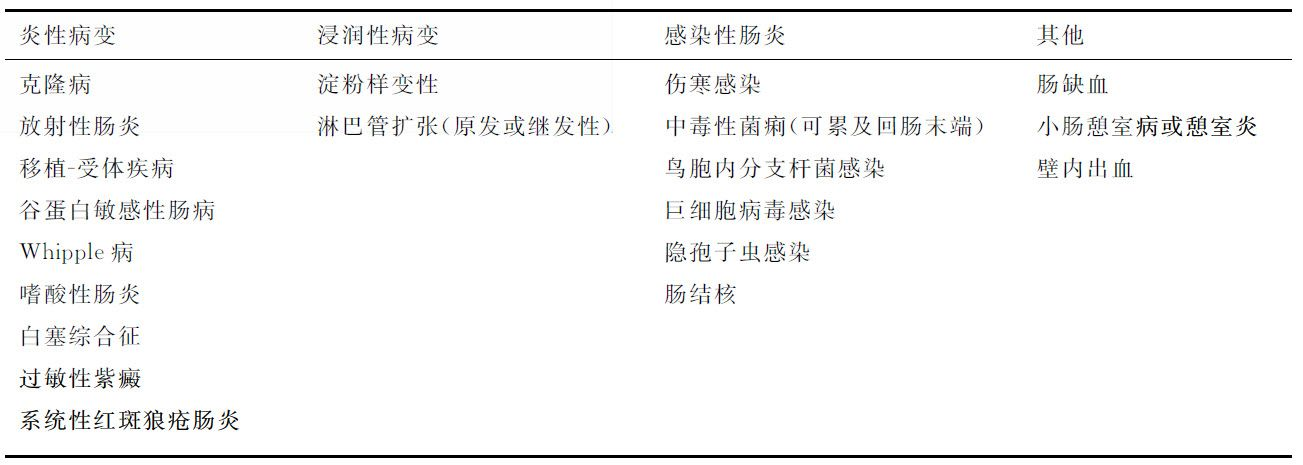
\includegraphics[width=\textwidth,height=\textheight,keepaspectratio]{./images/Image00363.jpg}
\end{table}

\subsubsection{小肠良恶性肿瘤的病理学分类}

①上皮性肿瘤:常见的有腺瘤和腺癌;②内分泌性肿瘤:主要指类癌;③非上皮性肿瘤:良性的如平滑肌瘤、脂肪瘤、血管和淋巴管肿瘤、神经源性肿瘤;恶性的主要有平滑肌肉瘤、卡波西(kaposi)肉瘤;④恶性淋巴瘤;⑤肿瘤样病变:如错构瘤、异位腺瘤、布氏腺增生、炎性纤维性息肉、Cronkhite-Canada综合征、淋巴滤泡增生、良性淋巴性息肉、回盲瓣的脂肪增生、子宫内膜异位症;⑥上皮的异型增生。

总之,良性最常见为平滑肌瘤,其次为腺瘤和脂肪瘤等。恶性以平滑肌肉瘤、腺癌、类癌、恶性淋巴瘤最多见。

\subsubsection{良性疾病的小肠壁增厚和双晕征}

小肠壁增厚可由炎症、血管疾病、肿瘤等所致。

导致小肠壁增厚且可出现“双晕征”或“靶征”的良性疾病主要有:Crohn病、缺血性肠炎、感染性肠炎、放射性肠炎、嗜酸性胃肠炎。过敏性紫癜(也称为Schonlein-Henoch血管炎或综合征)、小肠绞窄性或单纯性梗阻、SLE小肠炎、低蛋白血症及门静脉高压、小肠淋巴管扩张、移植-受体疾病(见于异体骨髓移植,主要累及皮肤、肝脏及胃肠道等,胃肠道腺上皮坏死和腺体减少)引起的肠水肿。此外,结肠的溃疡性结节炎、肠结核、中毒性菌痢亦可出现“双晕征”,而且后两者可累及回肠末端。

许多良性疾病可引起环状或对称性肠壁增厚,但通常<1cm。肠壁增厚即可表现为均匀软组织密度,又可表现为高低密度混杂的环状影,后者即所谓“双晕征”或“靶征”(图\ref{fig17-12})。肠出血则呈高密度增厚。双晕征是由于肠黏膜下水肿和(或)脂肪沉积等引起,于螺旋CT增强血管期观察最佳。

\begin{figure}[!htbp]
 \centering
 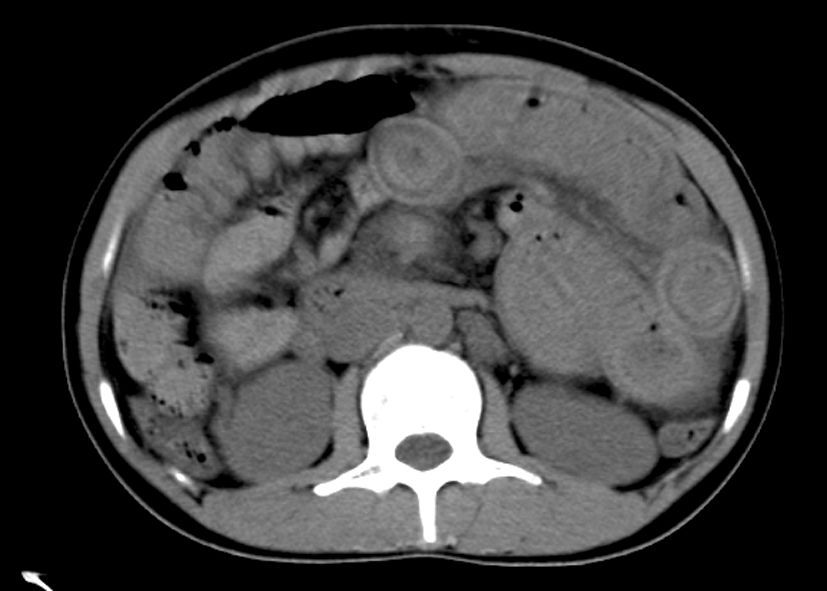
\includegraphics[width=.7\textwidth,height=\textheight,keepaspectratio]{./images/Image00364.jpg}
 \captionsetup{justification=centering}
 \caption{小肠壁双晕征\\{\small 左侧多处小肠壁水肿,呈双晕征}}
 \label{fig17-12}
  \end{figure} 

小肠良性疾病通常为节段性,病变处肠系膜脂肪多密度增高呈条状。

\subsubsection{小肠肿瘤的基本CT征象}

1.肿块与肠壁增厚:如①平滑肌瘤主要表现为肠壁偏心性增厚和肿块;②腺癌和淋巴瘤则多表现为全周性或局部的肠壁增厚;③类癌则常表现为靠近肠系膜侧的、轮廓清楚的肿块和星芒状的结节;④转移瘤:呈肠壁多发的软组织结节,也可形成肠系膜肿块或位于肠腔内的大息肉状肿块。

2.肠套叠和肠梗阻:是另一常见征象。成人的小肠套叠多由肿瘤所致。

此外,从发病部位看,腺癌多见于近侧小肠,并常引起梗阻;而淋巴瘤多见于回肠,并常伴有肠系膜或大动脉旁的淋巴结增大。

\subsection{克隆病(Crohn病)}

本病是一种原因不明的疾病,可累及胃肠道的任何部位,以末端回肠和右半结肠最常见。多节段发病和跳跃式分布为其特征。

\textbf{【病理】}
可分为炎症活动期、纤维化期、再生修复期。其病理特征为胃肠道的纵行溃疡、非干酪性肉芽肿性全层肠壁炎、纤维化和淋巴管阻塞。因淋巴水肿致肠壁增厚,黏膜表面有结节状隆起,呈铺路石样。黏膜可有多种形态的溃疡,早期为微小溃疡,继而有纵行线状溃疡。早期还有肉芽肿结节形成。病变呈多节段发病和跳跃式分布。晚期为肠壁纤维化导致肠壁增厚、管腔狭窄。

\textbf{【临床表现】}
本病多发生于成人,有时可发生于儿童。可以是急性的,也可是慢性的。其临床症状与并发症关系密切。急性发作时可像阑尾炎。常见症状为腹胀、腹泻、腹痛、低热、贫血、厌食和体重减轻等,可触及腹部包块。慢性症状常为肠梗阻表现,多系进行性加重。还可有肝脾肿大、关节炎、皮疹、虹膜炎、杵状指等肠外表现。

\textbf{【CT表现】}

1.急性期:无肠管狭窄者,表现无特征性。①仅表现为小肠皱襞增厚、模糊,小肠壁轻度增厚,壁厚可达10~11mm,可出现双晕征。②急性期增强扫描肠壁可呈4种增强方式:即多层(3层或更多)、2层强化(显著的黏膜强化和明显的黏膜下低密度称为双晕征)、肠壁显示2层但无明显的黏膜强化、均匀强化。③CT上小肠及结肠周围看到显著的血管影常提示处于活动进展期。主要表现为小血管的数量增加、扭曲,血管突然变细、直角分支,早期静脉强化和肠壁密度增高。④肠外改变及并发症的显示,如肠系膜受累、脓肿、瘘管、小肠梗阻、胰腺炎等。

2.慢性期:肠壁增厚是由纤维化所致。成层的双晕征消失,而表现为较均匀的软组织影伴肠腔狭窄。有以下特征:①病变多位于回肠末端,小肠和结肠可同时发病;②受累的肠壁呈节段性、对称性增厚,内外壁不规则,管腔狭窄或消失;③病变跳跃式分布;④晚期病例合并系膜改变,病变肠袢附近系膜脂肪密度增高形成肿块样高密度影,肠壁间距增大。

\textbf{【并发症】}
①脓肿:腹腔、腹壁脓肿;②窦道、瘘管:肠膀胱瘘、肠皮肤瘘、肛瘘和直肠阴道瘘;③肠梗阻。此外,本病与小肠和结肠腺癌、淋巴瘤的发生有密切关系。

\subsection{放射性肠炎}

本病是由于放疗后坏死性动脉炎所引起的肠壁黏膜和黏膜下层损伤,远段小肠最易受累。

\textbf{【病因病理】}
本病好发于手术后放疗病人,因手术可造成术野邻近的肠袢或与腹壁形成粘连,从而限制了小肠肠袢的运动,故易受到放射损伤。病理学早期表现为肠黏膜水肿、充血,以后肠壁血管栓塞,黏膜坏死、脱落形成溃疡。后期肠壁因纤维组织增生而增厚、肠腔变狭,附近系膜往往同时受累。

\textbf{【临床表现】}
可有恶心、呕吐和腹痛。但多无症状,常在随诊原发肿瘤的时候发现放射性肠炎的改变。

\textbf{【CT表现】}
急性者通常表现为肠壁增厚、水肿以及相邻肠系膜脂肪的炎性改变。慢性放射性肠炎在放疗后1~2年发生,以小肠袢固定增厚、硬化、瘘管形成为特点。

总之,本病CT表现无特异性,包括:①肠壁增厚(常伴有小溃疡);②肠袢因炎症浸润呈匐行狭窄,也可因肠壁增厚和水肿而骤然狭窄;③可出现双晕征,但该征是不均匀的。

\subsection{谷蛋白敏感性肠病}

本病亦称非热带性口炎性腹泻,是以小肠绒毛萎缩为特征,并可引起吸收功能紊乱、体重减轻、腹泻及贫血等症状的腹部病变。主要见于儿童和青年人。诊断要通过空肠活检,治疗方法是去除饮食中的谷蛋白。

\textbf{【CT表现】}
典型表现为小肠扩张,肠内积液增多使口服对比剂稀释。病变主要累及空肠的中、远段。还可见到小肠皱襞间距增宽及肠系膜淋巴结增大。

\textbf{【并发症】}
包括全身淋巴结增大、肠系膜淋巴结空洞综合征(淋巴结增大且伴中央低密度坏死区)和脾功能减退,也可发生肠套叠,而且伴发小肠淋巴瘤的和腺癌的几率增大。

\subsection{惠普尔(Whipple)病}

本病又称为肠道脂肪代谢障碍病。

\textbf{【病因病理】}
是革兰氏阳性菌感染引起的成人慢性多系统疾病。受累的小肠黏膜和黏膜下层有特征性的泡沫巨细胞浸润,泡沫巨细胞中含有周期性出现的酸-希夫反应阳性的糖蛋白颗粒。

\textbf{【临床表现】}
男性明显多于女性。临床特征为肠道吸收不良所致的体重减轻、脂肪泻和关节炎,还可有发热、贫血和淋巴结增大。其中65%~90%的病人有关节痛和(或)关节炎,常先于其他表现,多游走及反复发作,但不残留畸形(其关节改变归为血清阴性脊椎关节病范畴)。

\textbf{【CT表现】}
有国外文献认为小肠壁增厚、肠腔扩张不明显及肠内容物通过时间正常,伴有特征性的淋巴结出现对本病有定性诊断意义。其他表现还有肝、脾大和腹水。所谓特征性的淋巴结即肠系膜和腹膜后腔有成堆的巨大淋巴结,这些淋巴结内有低密度是由于包含的脂肪所致。

关节的X线表现为非特异性的周围关节改变,脊椎改变类似于类风湿性关节炎,可见骶髂关节硬化及单侧或双侧骶髂关节融合。

\subsection{嗜酸性胃肠炎}

本病是一种侵犯儿童和青年人的少见的过敏性疾病。

\textbf{【病因病理】}
其病因不明,50%有食物过敏史或过敏性疾病家族史。也有学者报道可由饮食不当(如暴饮暴食)、肠道及全身感染、药物所致。一般认为与Ⅰ型变态反应有关。病理上胃壁和(或)小肠壁有嗜酸粒细胞浸润,常伴其他部位的嗜酸粒细胞增多。

\textbf{【临床表现】}
以20~50岁多见。主要表现为腹痛、腹泻、恶心呕吐等症状,重者可有消化道出血。80%外周血中嗜酸粒细胞增高,IgE、IgG升高。其临床表现无特异性,确诊需以下4项标准:①有消化系统症状;②病理证实胃肠道1处或多处嗜酸粒细胞浸润;③排除胃肠道外多器官嗜酸粒细胞浸润;④无寄生虫感染。

\textbf{【CT表现】}
无特异性。可累及胃和诸段小肠,甚至盲肠和结肠,小肠壁可弥漫性增厚,增强扫描有强化。有文献认为常见远段胃壁和近段小肠黏膜皱襞结节状或不规则状增厚;如仅累及胃窦和近段小肠,有助于诊断。肠系膜炎性浸润和腹水亦不少见,但无特异性。当嗜酸性粒细胞侵及肠壁肌层时,可使肠袢僵硬,类似淋巴瘤或腺癌浸润,易造成误诊。

\subsection{肠道白塞综合征}

本病是以细小血管炎为病理基础的慢性进行性、复发性、多系统受侵的疾病。病因不明,可累及多个器官,包括胃肠道。

\textbf{【临床表现】}
多见于20~40岁男性,男女之比约2∶1。临床诊断标准:复发性口腔溃疡,加下述表现中的两项即生殖器溃疡、眼病(葡萄膜炎、视网膜脉管炎)、皮肤损害(结节性红斑、假性毛囊炎、丘疹脓疱疮性病变、痤疮性结节),或一项病理试验阳性(皮肤刺伤后24~48h内脓疱形成)。消化道可有腹痛、腹泻、便血等症状,确诊主要通过活检。

\textbf{【CT表现】}
肠道病变表现为肠管的炎症和溃疡,通常发生在回肠和盲肠。小肠黏膜皱襞增厚是典型表现,常为局限性、肿块样增厚,与小肠淋巴瘤或癌相仿。分散存在的胃肠道溃疡结合临床病史有助于诊断。

\subsection{腹型过敏性紫癜}

过敏性紫癜也称为Schonlein-Henoch血管炎或综合征,分为单纯型、腹型、关节型及肾型,是一种毛细血管变态反应性疾病,冬春季为好发季节。

\textbf{【病因病理】}
致敏源有食物、细菌感染、药物、花粉及寄生虫等。其病理特征为真皮层内毛细血管炎,血管壁可有灶性坏死及血小板血栓形成。胃肠道损害呈单发或多发节段性,最常见于空肠,毛细血管、小动脉、小静脉呈急性炎性反应,血管周围中性粒细胞和嗜酸粒细胞浸润、红细胞渗出,血管壁纤维样坏死,间质水肿。

\textbf{【临床表现】}
过敏性紫癜主要见于学龄前儿童,出现消化道症状者约占50%~60%,其中皮肤损害出现前有腹部症状者占12.7%。主要表现为腹痛、呕吐、腹泻及消化道出血。

\textbf{【CT表现】}
可见多发或单发的节段性肠壁水肿,对称或不对称性肠壁增厚,界限模糊不清,肠狭窄,部分可伴腹腔积液。增强扫描轻度均匀强化。较常见的并发症有肠套叠、穿孔和梗阻。

结合其临床症状和实验室检查,尤其结合其典型的皮肤损害和肾损害是CT诊断的关键。

\subsection{小肠淀粉样变性}

小肠淀粉样变性占全身性淀粉样变性的70%以上,发生在肠壁黏膜下层的小血管周围和黏膜层的纤维组织间。通过对受累器官的组织学检查确诊。

\textbf{【CT表现】}
表现为受累小肠壁弥漫性、均匀增厚。因小肠运动力下降,使造影剂通过时间延长,但肠管无明显扩张。也可有淋巴结增大或出现其他脏器(肝或肾)的淀粉样变,有助于鉴别诊断。偶可见肠壁钙化,具有特异性。

本病所致的淋巴结增大与Whipple病不同,通常不是巨块状的或低密度的。

\subsection{小肠淋巴管扩张}

本病是一种有严重失蛋白性水肿并伴有胸腹水的少见肠道病变。

\textbf{【病因病理】}
可以是原发性的(Milroy病),由先天性淋巴管阻塞引起;也可是继发性的,由淋巴管炎性或肿瘤性浸润所致。病理上小肠黏膜、黏膜下层及肠系膜内淋巴管扩张。

\textbf{【CT表现】}
无论原发性还是继发性均表现为肠壁浸润性增厚,这是由于小肠绒毛内淋巴管扩张使绒毛肿胀引起的。由于肠壁水肿也可见到双晕征。胸、腹水是其典型表现。肠系膜浸润以及主动脉旁或肠系膜淋巴结增大是继发性淋巴管扩张的征象,原发性淋巴管扩张多无淋巴结增大。

\subsection{小肠缺血}

随着人类平均寿命的延长肠缺血的发病率增高,据估计在急性腹痛的病例中1%为缺血性肠病。但其临床和病理学表现往往缺乏特征性,导致死亡率仍然很高,其中急性肠缺血死亡率可达50%~90%。

\textbf{【病因】}
可以是肠系膜动脉堵塞或静脉血栓形成,也可因心输出量减少(如低血压、脓毒血症、心衰、洋地黄治疗)或动脉粥样硬化所致血液灌注减少。肠缺血更常继发于机械性肠梗阻(包括闭袢性肠梗阻、疝和肠套叠)后的脉管损伤。总之,其病因包括多方面:①动脉血流减少或闭塞;②静脉血流减少或闭塞;③低血流量状态。

根据缺血的发生时间及临床表现分为急性和慢性。国外报道肠系膜上动脉栓塞或血栓形成占急性肠缺血的60%~70%,肠系膜静脉血栓形成占5%~10%,非阻塞性占20%~30%;而慢性缺血大多来自肠系膜动脉粥样硬化。

\textbf{【病理】}
急性肠缺血可分为3期:第1期:又称可逆性小肠炎或结肠炎。以黏膜坏死、糜烂、出血为特征。病变通常局限于黏膜层,可自愈。第2期:肠壁损害达到黏膜下层和肌层,可产生局部纤维性狭窄。第3期:透壁性肠坏死即梗死,临床死亡率高,需立即手术或介入治疗。

\textbf{【临床表现】}
发病年龄多在50岁以上。可表现为腹部轻微不适或急性腹痛等症状,临床诊断极为困难。急性者有突发性剧烈腹痛、恶心和呕吐、腹泻和血便等,严重者可出现休克。慢性者大多数是吸烟者,1/3以上有高血压、冠心病和脑血管病;典型表现为反复的上腹部或中腹部餐后腹痛,1~2小时后缓解;大多数还可出现体重下降。

\textbf{【CT表现】}
所有小肠均可受累,但以远端小肠多见,肠系膜上动脉阻塞能使大部分小肠和右半结肠受累。早期常表现为肠内积液、扩张,伴有或不伴有肠壁增厚。病变进展时,肠壁增厚可达5~10mm,可见双晕征,肠系膜因水肿或出血而模糊。当肠壁、门静脉或肠系膜血管内出现积气时,通常是晚期表现,并提示肠梗死。但肠壁增厚在梗死时反而少见。增强扫描可见受累肠段增厚的肠壁强化不明显或不强化,如在肠系膜动脉或静脉内出现灶性积气或栓子(血管内充盈缺损)可做出特异性诊断。慢性肠缺血多为肠系膜动脉粥样硬化所致的管腔狭窄,由于病程长多建立起侧支循环,故除非并急性血栓栓塞,小肠形态通常正常。

此外,休克肠是由于创伤等引起低血压病人的广泛性小肠病变。CT表现肠管明显扩张、积液;增强扫描肠壁明显强化且多持续数分钟,是由于循环血量减少造影剂浓度相对升高所致。还可见下腔静脉和(或)主动脉管径变小,肾、胰和肠系膜明显强化。

总之,急性期直接征象是血管内充盈缺损,间接征象是肠壁增厚,肠管扩张,肠系膜水肿、积液和腹水;肠壁密度异常(多为低密度,亦可因出血淤血而呈高密度)、肠壁积气和门静脉内积气、肠系膜血管改变。慢性期可表现为肠管狭窄。但需与肠痉挛、感染性炎症相鉴别,可鉴别困难。

\subsection{小肠壁内出血}

\textbf{【病因】}
小肠出血的原因很多,包括肠缺血、创伤、血管炎、凝血缺陷以及抗凝治疗。出血发生于黏膜下层,由于病因不同,病变范围可以是弥漫或局限。

\textbf{【CT表现】}
肠壁规则增厚、壁内肿块以及肠腔狭窄,急性者呈高密度血肿。如对本病认识不足,可误诊为小肠肿瘤。

\subsection{空回肠憩室}

本病并不多见,可分为先天性和后天性。

\textbf{【病因病理】}
其病因尚不明确。①先天性憩室:包括美克尔憩室和肠重复畸形中一段肠管的一段闭塞所形成的憩室。②后天性憩室:较先天性多见。肠系膜血管进入肠壁处较为薄弱,由于肠蠕动及肠内容物的关系可使肠管内压力增高,久之可使薄弱处的肠壁外突形成憩室。病理上憩室壁包含肠壁的黏膜层、肌层及浆膜层。可并发憩室炎,甚至可发生穿孔引起腹膜炎。

\textbf{【临床表现】}
多无症状。发生憩室炎时可有食欲不振、恶心、呕吐、腹痛,甚至腹泻等症状,可并发肠梗阻、憩室穿孔和出血等。

\textbf{【CT表现】}
肠腔局部外突,内容对比剂或气体,如果肠腔内有足够对比剂则更易于发现。其中美克尔憩室表现为中下腹小囊肿,多呈圆锥形或圆柱形,长3~4cm,直径1~2cm。6%~10%的小肠憩室有急性并发症,包括穿孔、肠梗阻、出血和憩室炎。

\subsection{肠重复畸形}

消化道重复畸形系紧密附着于消化道的球形或管状空腔器官,具有消化道结构,并与主肠(胃)管有着共同的血供。其发病部位以回肠及回盲部多见,约占50%~70%,其次为大肠、空肠、食管、胃、十二指肠。其病因及发病机理存在着多源性。

\textbf{【病理】}
重复畸形壁层中含有分化完全的消化道各层结构,其中黏膜层约20%~50%有异位黏膜。约80%重复畸形内腔与所附消化道不通。肠重复畸形的基本病理类型包括肠内囊肿型、肠外囊肿型、管状型、胸内型,其中肠外囊肿型最多见,约占80%。

\textbf{【临床表现】}
多在新生儿或婴儿期发现。主要表现为腹部肿块,以及因黏膜分泌的消化液腐蚀囊壁产生消化性溃疡或异位组织中的胰腺炎所引起的症状,包括呕吐、腹痛和消化道出血等。还可有肠梗阻、腹膜炎以及伴发的其他畸形。

\textbf{【影像学表现】} 缺乏特异性。

1.平片及钡餐或钡灌肠:表现为腹部肿块、肠腔内充盈缺损或肠管受压移位,可伴有脊柱畸形。如与主肠管相通则可见钡剂进入其中,且排空延迟。部分或全结肠重复畸形表现为并行的双排管状结构。

2.CT表现:低密度单房囊性肿块,大多为球形,多与肠管不通;有些呈管状,可与肠管相通。重复畸形的壁厚与毗邻肠管壁相近或更厚。部分囊壁可钙化。增强扫描囊壁可强化。

\textbf{【鉴别诊断】}
本病需注意与系膜网膜囊肿、美克尔憩室、胆总管囊肿、假性囊肿、卵巢囊肿及腹腔脓肿等相鉴别。

\subsection{小肠良性肿瘤}

\subsubsection{平滑肌瘤}

本病占小肠肿瘤的首位。

\textbf{【病理】}
多为单发,多发少见。其生长方式有4种:壁内、黏膜下、浆膜下、哑铃型生长。较大者内部因缺血而出现坏死、囊变,表面可有溃疡。镜下平滑肌瘤无核分裂、异形性不明显。

\textbf{【临床表现】} 一般仅50%有症状,表现为腹部包块、黑便、贫血等。

\textbf{【CT表现】}
肿瘤呈偏心性生长的圆形或椭圆形肿块,边缘光滑清晰,直径多<5cm。肿瘤密度多均匀、边缘多光整;直径>4cm时,中心部多可见低密度坏死、囊变区。浆膜下者可见邻近肠袢的移位。由于富血供,增强扫描显著强化。

\subsubsection{腺瘤}

本病是最常见的小肠黏膜肿瘤,约占小肠良性肿瘤的25%。本病好发于十二指肠及空肠。

\textbf{【病理】}
肿瘤单发或多发。多发者可累及一段或整个小肠,甚至整个消化道。肿瘤向腔内生长,有蒂或无蒂,位于黏膜下,大小不一,易癌变。

\textbf{【临床表现】} 多无明显症状,也可有腹痛,易引起肠梗阻和出血。

\textbf{【CT表现】}
肠腔内圆形软组织结节或肿块,密度均匀、边缘光滑,有时可呈菜花状;在造影剂衬托下形成充盈缺损。肿瘤邻近的肠壁无增厚,如有增厚则多为腺癌。此外应注意小的腺瘤CT检出率低(约20%)。

\subsection{小肠脂肪瘤}

消化道脂肪瘤多见于结肠和小肠,约占小肠肿瘤的15%,发病率仅次于平滑肌瘤和腺瘤,居小肠肿瘤的第3位。

\textbf{【病理】}
境界清楚的脂肪组织肿块,多起源于黏膜下层脂肪组织,膨胀性生长,也可发生于浆膜下突出于肠壁外。多单发,大小不一。

\textbf{【临床表现】}
肿瘤小时无症状,大者可出现急性和亚急性痉挛腹痛、恶心、呕吐、腹泻。易引起肠套叠,出现梗阻和便血等症状。

\textbf{【CT表现】}
表现为与肠管关系密切的脂肪密度肿块,CT值约-50~-120Hu,密度均匀。邻近肠壁不增厚。如继发肠套叠,勿将肠套叠内的肠系膜脂肪影与脂肪瘤相混淆,还应区别回盲瓣的脂肪沉积。

\subsection{小肠恶性肿瘤}

\subsubsection{腺癌}

本病以十二指肠最多见(50%),尤以降部为甚,其次为空肠。

\textbf{【病理】}
可分为肿块型和浸润型。肿块型向肠腔内呈息肉状生长;浸润型沿肠壁浸润,易造成肠腔狭窄和梗阻。

\textbf{【临床表现】}
常见症状为腹痛、恶心呕吐、少量消化道出血、腹块、不同程度肠梗阻或肠套叠。

\textbf{【CT表现】}
最常见的表现为局灶性肿块伴相邻肠壁增厚,肠管环状或偏心性狭窄。增强扫描呈中度强化,密度不均。少数呈境界清楚的巨大肿块,且无梗阻。肝脏、腹腔、卵巢和淋巴结转移率较高,且易继发肠梗阻(完全性或不完全性)或肠套叠。

\subsubsection{平滑肌肉瘤}

不同于腺癌,常位于回肠,占50%以上;空肠次之,占37%;十二指肠仅占10%。

\textbf{【病理】}
肿瘤倾向于向肠腔外生长,肿块往往较大,而较少产生肠梗阻。肿瘤呈类圆形,中心易出现坏死、囊变,表面常有溃疡,甚至形成窦道。镜下平滑肌肉瘤有不用程度的核分裂、异形性明显,如核的多形性、核大而浓染。

\textbf{【临床表现】}
常见症状为腹痛、恶心呕吐、少量消化道出血、腹块,较少引起肠梗阻。

\textbf{【CT表现】}
肿瘤多向肠腔外生长,位于肠壁间;直径一般>5cm,甚至达10cm以上。肿瘤无固定形态,可呈分叶状或不规则形。肿块密度多不均匀,中心常有坏死、囊变,以及溃疡、瘘管,可伴液气平面。肿块的巨大坏死囊腔内充盈造影剂且与肠腔相通为其特征性表现,钙化少见。增强扫描周边显著强化。偶呈无明确边界的浸润性生长,与淋巴瘤和腺癌相似。淋巴结转移少见;肝转移呈囊样,牛眼征较多见。

\subsubsection{类癌}

本病约占小肠肿瘤的1/3。好发于回肠,尤其远端回肠,可多发。

\textbf{【病理】}
源于肠黏膜腺体的嗜银细胞,有潜在分泌多种不同的多肽类及活性胺类激素的功能。肿瘤多小于1.5cm,较大可有表面溃疡,伴局部肠壁增厚。

\textbf{【临床表现】}
发生于空回肠者常有典型的临床表现,如皮肤潮红、毛细血管扩张、恶心、支气管哮喘、腹痛、腹泻、便血、腹部包块等。靠近十二指肠者较少分泌激素,主要表现为梗阻和局部感染。

\textbf{【CT表现】}
表现为小的黏膜下肿块,可有钙化。因原发灶多较小而不易显示。肠系膜转移灶呈星芒状(放射状)肿块,直径2~5cm,密度均匀,有一定特异性。放射状肿块系纤维反应性增生向肿瘤部位纠集的结果。肿瘤穿破肠系膜时,还可导致肠粘连和梗阻。常见肝转移,但罕见钙化;偶有腹水;亦可见淋巴结转移,并作为惟一表现而误为淋巴瘤。

\subsection{小肠恶性淋巴瘤}

本病占小肠恶性肿瘤的20%~50%,在胃肠道淋巴瘤中占35%~70%,以NHL多见。可为原发,也可为全身淋巴瘤的一部分。

\textbf{【病理】}
起源于黏膜下淋巴组织,其发展向外可侵入浆膜层、肠系膜及其淋巴结。最易受累的部位是远段小肠,其次是空肠,十二指肠最少见,偶见多发者。

\textbf{【临床表现】}
发病年龄较轻,多在40岁左右。主要症状为腹痛,其次为不规则发热、恶心、呕吐和厌食等,半数以上体重减轻,部分可触及肿块。少见的症状有间歇性便血、肠穿孔、腹泻、便秘和肠梗阻等。

\textbf{【CT表现】}
可分为5型:①多发结节型;②壁内浸润型;③息肉样肿块型;④伴瘘管形成的肠内肠外型;⑤肠系膜受累伴腔外肿块型。

其中:①前3种类型表现为小肠壁的局限不均匀增厚,但较小肠癌范围长,单发为主;或呈向腔内突出的软组织密度肿块。壁外轮廓完整,与周围肠管分界清。②肿块较大时(为后两型),可显示相邻肠管的推移、粘连及浸润,甚至累及系膜。③肿瘤有溃疡形成或内部坏死可形成与肠腔相通的窦道,进而可发展成瘘管。④有时可见肠管呈“动脉瘤样”扩张,且有文献认为是回肠淋巴瘤的特征性表现。⑤肠系膜受累多表现为结节状肿块,肠系膜和腹膜后的淋巴结可显著增大,并包绕肠系膜血管及其周围脂肪,形成所谓的“三明治”征。

综上所述,其CT表现为肠壁增厚(环形强化)、肠腔变形、肠管扩张或狭窄、腹部肿块、肠管周围淋巴结增大。此外,继发性者还可见腹膜后、肝门、脾门等处淋巴结增大等。

\textbf{【鉴别诊断】}

1.平滑肌肉瘤:小肠恶性淋巴瘤有时可表现为腹腔内肿块,CT上与平滑肌瘤或平滑肌肉瘤相似。但仔细观察肿块内可见肠道内的气体影和对比剂,病变范围广泛,强化不明显;而平滑肌瘤或肉瘤的肿块内可见囊变或坏死区,一般没有被包绕的肠道内的气体或对比剂,病变范围较局限,强化明显。

2.小肠癌:主要表现为肠腔狭窄或肿块,病变肠管无扩张,病变相对局限。有学者认为淋巴瘤胃(肠)壁的淋巴细胞增殖没有破坏正常细胞,因而无成纤维反应,故胃(肠)腔缩小或梗阻相对胃(肠)癌少见。

3.克隆病:可类似淋巴瘤,但病变呈跳跃式分布等有助于鉴别。

4.小肠结核:可有肠壁增厚、肠管周围淋巴结增大而类似淋巴瘤。但结核一般好发于回盲部,无肠管扩张,结合消化道造影可见激惹征等可资鉴别。

\subsection{小肠转移瘤}

本病产生途径有:①血行转移:见于多血供的肿瘤,如肺癌、乳癌、恶性黑色素瘤、卡波西肉瘤等;②种植转移:多来源于腹腔或盆腔含黏液成分较多的肿瘤,如卵巢、阑尾、结肠、直肠等部位;③直接浸润:如肾、肾上腺、胰腺等肿瘤。

\textbf{【临床表现】}
无特异性,可犹如消化功能紊乱。还可表现为腹块、腹痛、恶心呕吐、出血,亦可引起肠梗阻。与多发性的原发肿瘤如淋巴瘤、腺癌可难以鉴别,故结合病史对转移瘤的诊断甚为重要。

\textbf{【CT表现】}
①可在肠壁内形成黏膜下转移结节,大者可致肠梗阻和肠套叠。②有的肿瘤可出现溃疡和空洞。③沿肠壁弥漫浸润者可引起小肠壁的增厚,造成肠腔的不规则狭窄。④含黏液较多的肿瘤可在浆膜、肠系膜和网膜上形成多发结节,并在肠系膜和腹腔脂肪内浸润,造成密度增高和肠系膜血管束增粗;网膜受累时可见“网膜饼征”;并可伴腹水。⑤血行转移亦可在肠系膜上形成较大的肿块。⑥周围脏器肿瘤对小肠的直接浸润,表现为与原发灶相连续的不规则团块影。

\section{大肠疾病}

\subsection{溃疡性结肠炎}

本病是一种原因不明的、主要发生于结肠黏膜层的炎症性病变,以溃疡糜烂为主。

\textbf{【病因病理】}
其病因尚不明了,多认为与免疫异常、感染、遗传等因素有关。本病从直肠开始,以后逐渐向上发展,可累及整个结肠。早期病变多为局部结肠黏膜广泛性充血水肿和溃疡形成。溃疡间黏膜面呈颗粒状,残存未被破坏的黏膜大量增生,形成较大的炎性息肉。病变愈合时,黏膜下层有大量纤维组织增生形成瘢痕,可使肠腔变窄、肠管缩短,形似直筒状。

\textbf{【临床表现】}
多见于青壮年。以血性黏液便、腹痛、里急后重、腹泻为主要症状,也可有发热、贫血、消瘦等全身症状。常缓解与发作交替出现。可合并关节炎、皮肤病、口腔溃疡、肝病、虹膜炎等。

\textbf{【CT表现】}
急性期出现中毒症状时,表现肠管显著扩张达5cm以上,肠壁变薄。黏膜增厚和肠腔狭窄是亚急性期和慢性期的主要征象。本病主要有以下表现:①肠壁轻度增厚,常<1cm,外形大多光滑,少数也可不规则。肠腔稍狭窄,但轻于克隆病。②在结肠轴位像上可见双晕征或靶征,其中间的低密度层为黏膜下水肿(CT值多在10Hu以下)或脂肪沉积(-10Hu以下)。但此征亦可见于克隆病、中毒性菌痢等病变。③可见增厚的肠壁内溃疡,但轻微黏膜改变和表浅溃疡不易显示。④肠系膜和直肠周围间隙的脂肪浸润和纤维化;邻近可见淋巴结增大。⑤慢性者还可见直肠狭窄及直肠周围间隙增宽。⑥病史15年以上者癌变率为5%~10%,表现为肠壁不对称增厚,肠壁分层现象的消失,肠壁增厚>1.5cm。

\textbf{【鉴别诊断】}
与克隆病有时鉴别困难,以下几点有助于鉴别。①肠壁分层现象多见于溃疡性结肠炎(65%);少见于克隆病(8%)。②溃疡性结肠炎的肠壁厚度平均为7.8mm;而克隆病的肠壁则更厚,平均11mm。③绝大多数(95%)溃疡性结肠炎的浆膜面光滑规则;而大多数(80%)克隆病的浆膜面不规则。④溃疡性结肠炎病变从直肠开始,向近端肠管发展,呈连续性分布;而克隆病约50%不累及直肠,病变不连续,呈跳跃式发展。⑤溃疡性结肠炎的溃疡间黏膜可呈颗粒状增生;而克隆病黏膜面不呈颗粒状。

\subsection{结肠结核}

本病比较常见,其病理和临床症状与小肠结核类似。

\textbf{【病理】}
本病多自回盲部开始,向上延及升结肠,其次为横结肠,左半结肠少见。结肠系膜常受累,大多增厚、粘连收缩,使盲肠缩短。可分为两型:①溃疡型:可穿透浆膜层形成脓肿及瘘管;②增殖型:由于纤维增生而致肠壁增厚、管腔狭窄。

\textbf{【临床表现】}
以20~40岁多见,女性多与男性。可有结核中毒症状,以及腹痛,腹泻、便秘交替发生,可有梗阻症状和腹部包块。化验常见血沉增快。

\textbf{【CT表现】}
盲肠壁及其他肠区壁增厚,其密度不一或呈混杂密度。由于肠壁增厚而肠腔狭窄、狭窄近端肠管扩张。亦可因溃疡导致肠管边缘不规则。邻近系膜受累可形成不规则包块。继发肠梗阻有相应表现。

\textbf{【鉴别诊断】}
本病与克隆病、其他炎性病变以及结肠癌可不易鉴别。需密切结合临床进行鉴别。

\subsection{假膜性结肠炎}

本病少见。常由于长期使用广谱抗生素,造成肠道菌群失调所致。

\textbf{【病因病理】}
病原菌为梭状芽孢杆菌。该菌在正常情况下存在于肠腔内,当菌群失调时出现异常增生,产生毒素可引起肠黏膜上皮细胞变性坏死,坏死的肠黏膜和渗出的纤维素形成假膜,假膜脱落后可形成表浅不规则溃疡。本病还可由尿毒症、缺血和重金属中毒等因素所致。

\textbf{【临床表现】} 可表现为腹痛、腹胀、腹泻、脓血便等症状。

\textbf{【CT表现】}
无特异性。呈不典型的结肠扩张、肠壁增厚和结肠袋水肿。增强扫描可见肠壁的强化和浆膜面的肥厚,常伴小肠的扩张。肠壁内气体和腹水并不常见。

\subsection{放射性结肠炎}

本病主要见于盆腔肿瘤的放射治疗后,多在治疗后数周及数月发病。

\textbf{【病理】}
早期表现为肠黏膜水肿、充血,以后肠壁血管栓塞,黏膜坏死、脱落形成溃疡。后期肠壁因纤维组织增生而增厚、肠腔变狭,附近系膜往往同时受累,有时可有瘘管形成。

\textbf{【临床表现】}
主要为腹泻、便血、大便中带有大量黏液、腹痛和腹胀等。部分可出现肠梗阻症状。

\textbf{【CT表现】}
①急性期:表现为肠腔痉挛狭窄,肠壁轻度增厚,可有双晕征。②慢性期:出现肠腔狭窄、肠管变形,邻近系膜密度增高。伴发肠梗阻时出现相应表现。

此外,慢性期可伴直肠周围异常。①直肠周围脂肪增生,伴骶前间隙增宽>1cm;②直肠周围筋膜增厚、纤维组织增多,特别直肠旁间隙产生“晕圈”效应。但应注意如直肠壁或直肠周围有边缘清晰的软组织肿块,应提示有肿瘤残存和复发可能,需随访或穿刺活检予以鉴别。

\subsection{结肠缺血}

肠缺血根据发病部位可分为3类:①肠系膜缺血:病因包括动脉或静脉血流减少或闭塞、低血流量状态;②结肠缺血;③其他:机械性和绞窄性梗阻、休克肠。

\textbf{【病因病理】}
结肠缺血是老年人最常见的肠血管性疾病,又称为缺血性结肠炎。大多找不到确切的病因,也无血管闭塞的证据。因多发病于70岁以上,且常伴广泛的动脉硬化,故多认为是结肠血流减少所致。非闭塞性缺血常较动脉粥样硬化栓子所致的缺血累及范围大。非闭塞性结肠缺血一般累及结肠的交界区,即脾区、直肠乙状结肠交界处,但任何一段结肠均可受累。修复时受累肠段纤维化,严重时可导致肠腔狭窄。

\textbf{【临床表现】}
发病年龄多在50岁以上。与肠系膜缺血相比,结肠缺血的病人临床表现较轻。常诉轻微腹痛或血性腹泻。严重时也可出现休克。

\textbf{【CT表现】}
最常见的表现为结肠壁增厚,多为节段性受累,平均受累总长度为19cm。肠壁密度均匀,少数肠壁有分层现象。肠壁积气、肠系膜血管或门静脉积气提示肠壁全层缺血或梗死。增强扫描病变肠段不强化。

但某些其他良性病变、AIDS晚期也可出现类似征象。

\subsection{结肠憩室}

本病好发于乙状结肠和降结肠,亦可波及全部结肠。

\textbf{【病理】}
常发生于结肠系膜侧边缘。憩室壁缺乏肌层,易发生感染或憩室炎,便可形成腹腔窦道、瘘管、脓肿及肠粘连。

\textbf{【临床表现】}
多见于40岁以上男性。不发生炎症时无症状,伴憩室炎时有腹痛、腹胀、低热和白细胞升高等。憩室穿孔形成脓肿时,腹痛加剧、高热、下腹包块以及出现腹膜炎症状。

\textbf{【CT表现】}

1.结肠憩室表现为细颈样结构凸出于结肠壁外,其内可充盈空气、液体、造影剂或粪便等。

2.结肠周围脂肪的炎性浸润:表现为结肠周围脂肪内出现密度增加的软组织影,界限模糊,并伴有细线样、索条状影。

3.局部肠壁增厚超过4mm。

4.增厚的结肠壁内有液体和(或)造影剂聚集,表明有肠壁内窦道形成。

5.与憩室炎有关的盆腔脓肿、盆腔外脓肿和(或)腹膜炎。

6.窦道形成,尤其是乙状结肠-膀胱瘘。

\subsection{肠壁气囊肿}

本病为良性经过,偶尔表现为自限性。本病与肠壁内积气不同。

\textbf{【病因病理】}
本病的病因及发病机制尚不清楚,分为原发性和继发性。后者与胃肠道梗阻、慢性阻塞性肺疾病、结缔组织病等有关。原发性者多侵及左半结肠。其病理特征是胃肠道壁的黏膜下层和(或)浆膜下层出现大量气囊堆积。气囊破裂形成自发性气腹。

\textbf{【临床表现】}
一般无症状。症状多出于原发的肺或胃肠道病变,但有时可有腹痛、腹泻、便血等。

\textbf{【影像学表现】}
平片表现为肠壁堆积的大量蜂窝状气体影,结肠双重造影表现为多发的、光滑的黏膜下隆起,呈圆形或椭圆形。CT用肺窗观察可清晰地显示分布于肠壁的大量气囊状影。

\subsection{结肠腺瘤性息肉}

本病与增生性的炎性息肉不同,属肿瘤性病变,但影像学表现相近。腺瘤性息肉以及炎性息肉好发于直肠和乙状结肠,亦可发生于整个胃肠道。

\textbf{【病理】}
分为管状腺瘤、管状绒毛腺瘤和绒毛状腺瘤3种。息肉的大小与恶变密切相关;>2cm的息肉恶变率可在50%以上,<1cm的为2%~10%,而<0.5cm者罕有恶变。其中绒毛状腺瘤好发于老年人,易出血、癌变率极高。

\textbf{【临床表现】}
无痛性慢性便血为直肠、结肠息肉的特征。便血为间歇性,多量少;血色鲜红,覆盖在粪便上,不与其混合。继发感染时,还可有黏液脓便。息肉可诱发肠套叠,尤其位于末端回肠和盲升结肠者。

\textbf{【CT表现】}

1.管状腺瘤或管状绒毛腺瘤:通常呈较小的球形,有蒂或无蒂。如肿瘤较大(≥1.0cm),且分叶明显时,应提示有恶性变可能;如邻近肠壁增厚对恶性变有一定的诊断价值。

2.绒毛状腺瘤:多无蒂,基底宽,表面有许多叶状突起,病灶大小为3~9cm,甚至达15cm。其特征性CT表现为直肠肿块内有均质性水样密度影(CT值小于10Hu,由大量黏液集聚而成),常偏向肿块一侧,占病灶的一半以上。

\subsection{直肠血管瘤}

本病极少见,其中以海绵状血管瘤最常见。

\textbf{【临床表现】}
常见于年轻人。有急性或慢性反复发作的无痛性直肠便血,有时可有里急后重或便秘症状。

\textbf{【CT表现】}
可呈分散的息肉状黏膜下肿块或弥漫性浸润病变。肠壁内静脉石的显示是本病的特异性征象,否则不易诊断和鉴别。

\subsection{大肠子宫内膜异位症}

子宫内膜异位症30%发生于肠道,最常见于直肠乙状结肠交界处,亦可发生于其他部位如乙状结肠、盲肠、阑尾,小肠也可有种植。

\textbf{【临床表现】}
主诉随月经周期发作的痉挛性下腹部或盆区疼痛、直肠便血、里急后重等。

\textbf{【CT表现】}
无特异性。可表现为浆膜、浆膜下或黏膜下息肉状肿块或囊实性占位,以及肠壁轮廓的改变。

\subsection{结肠癌}

大肠癌为常见的消化道癌肿,其发病率仅次于胃癌、食管癌居第3位。以乙状结肠和直肠最多见,约占50%以上,其次为盲肠、升结肠,再次为降结肠及肝、脾曲结肠,横结肠最少见。本病与息肉病、血吸虫病、溃疡性结肠炎等有明显关系。

\textbf{【病理】}

1.组织学类型:以腺癌最常见,其他尚有黏液癌、乳头状腺癌、胶样癌、类癌和腺鳞癌等。

2.大体类型:①国内分为4类:增生型(肿块型)、浸润型、溃疡型、混合型。②国外将近展期大肠癌分为与胃癌相对应的BorrmannⅠ~Ⅳ型。

3.转移途径:①直接浸润;②淋巴转移;③血行转移;④种植转移。

\textbf{【临床表现】}
常见的症状为腹部肿块、便血、腹泻或有顽固性便秘、肠梗阻,也可有脓血便与黏液样便,以及全身乏力、体重减轻和贫血等。

\textbf{【CT表现】}

1.早期:可无异常表现,或表现为局限性肠壁增厚,而周围肠壁正常。

2.中晚期:表现多样化:①肠腔内偏心性分叶状肿块(图\ref{fig17-13})。②环形或半环形肠壁增厚。③肠腔狭窄和不规则。④广泛浸润者可使肠壁广泛僵硬,肠腔狭窄呈革囊袋状。⑤黏液腺癌病灶密度低,可见水样密度区;肝转移灶和增大的淋巴结也表现为低密度,偶见钙化灶。⑥肿瘤穿透肠壁达浆膜层和向外扩展时肠壁显得模糊。⑦可直接侵及周围脏器如胃、胰腺、胆囊、腹壁,盆腔内脏器及盆壁。⑧局部和腹膜后淋巴结转移。⑨肝脏及其他脏器的血行转移。

\begin{figure}[!htbp]
 \centering
 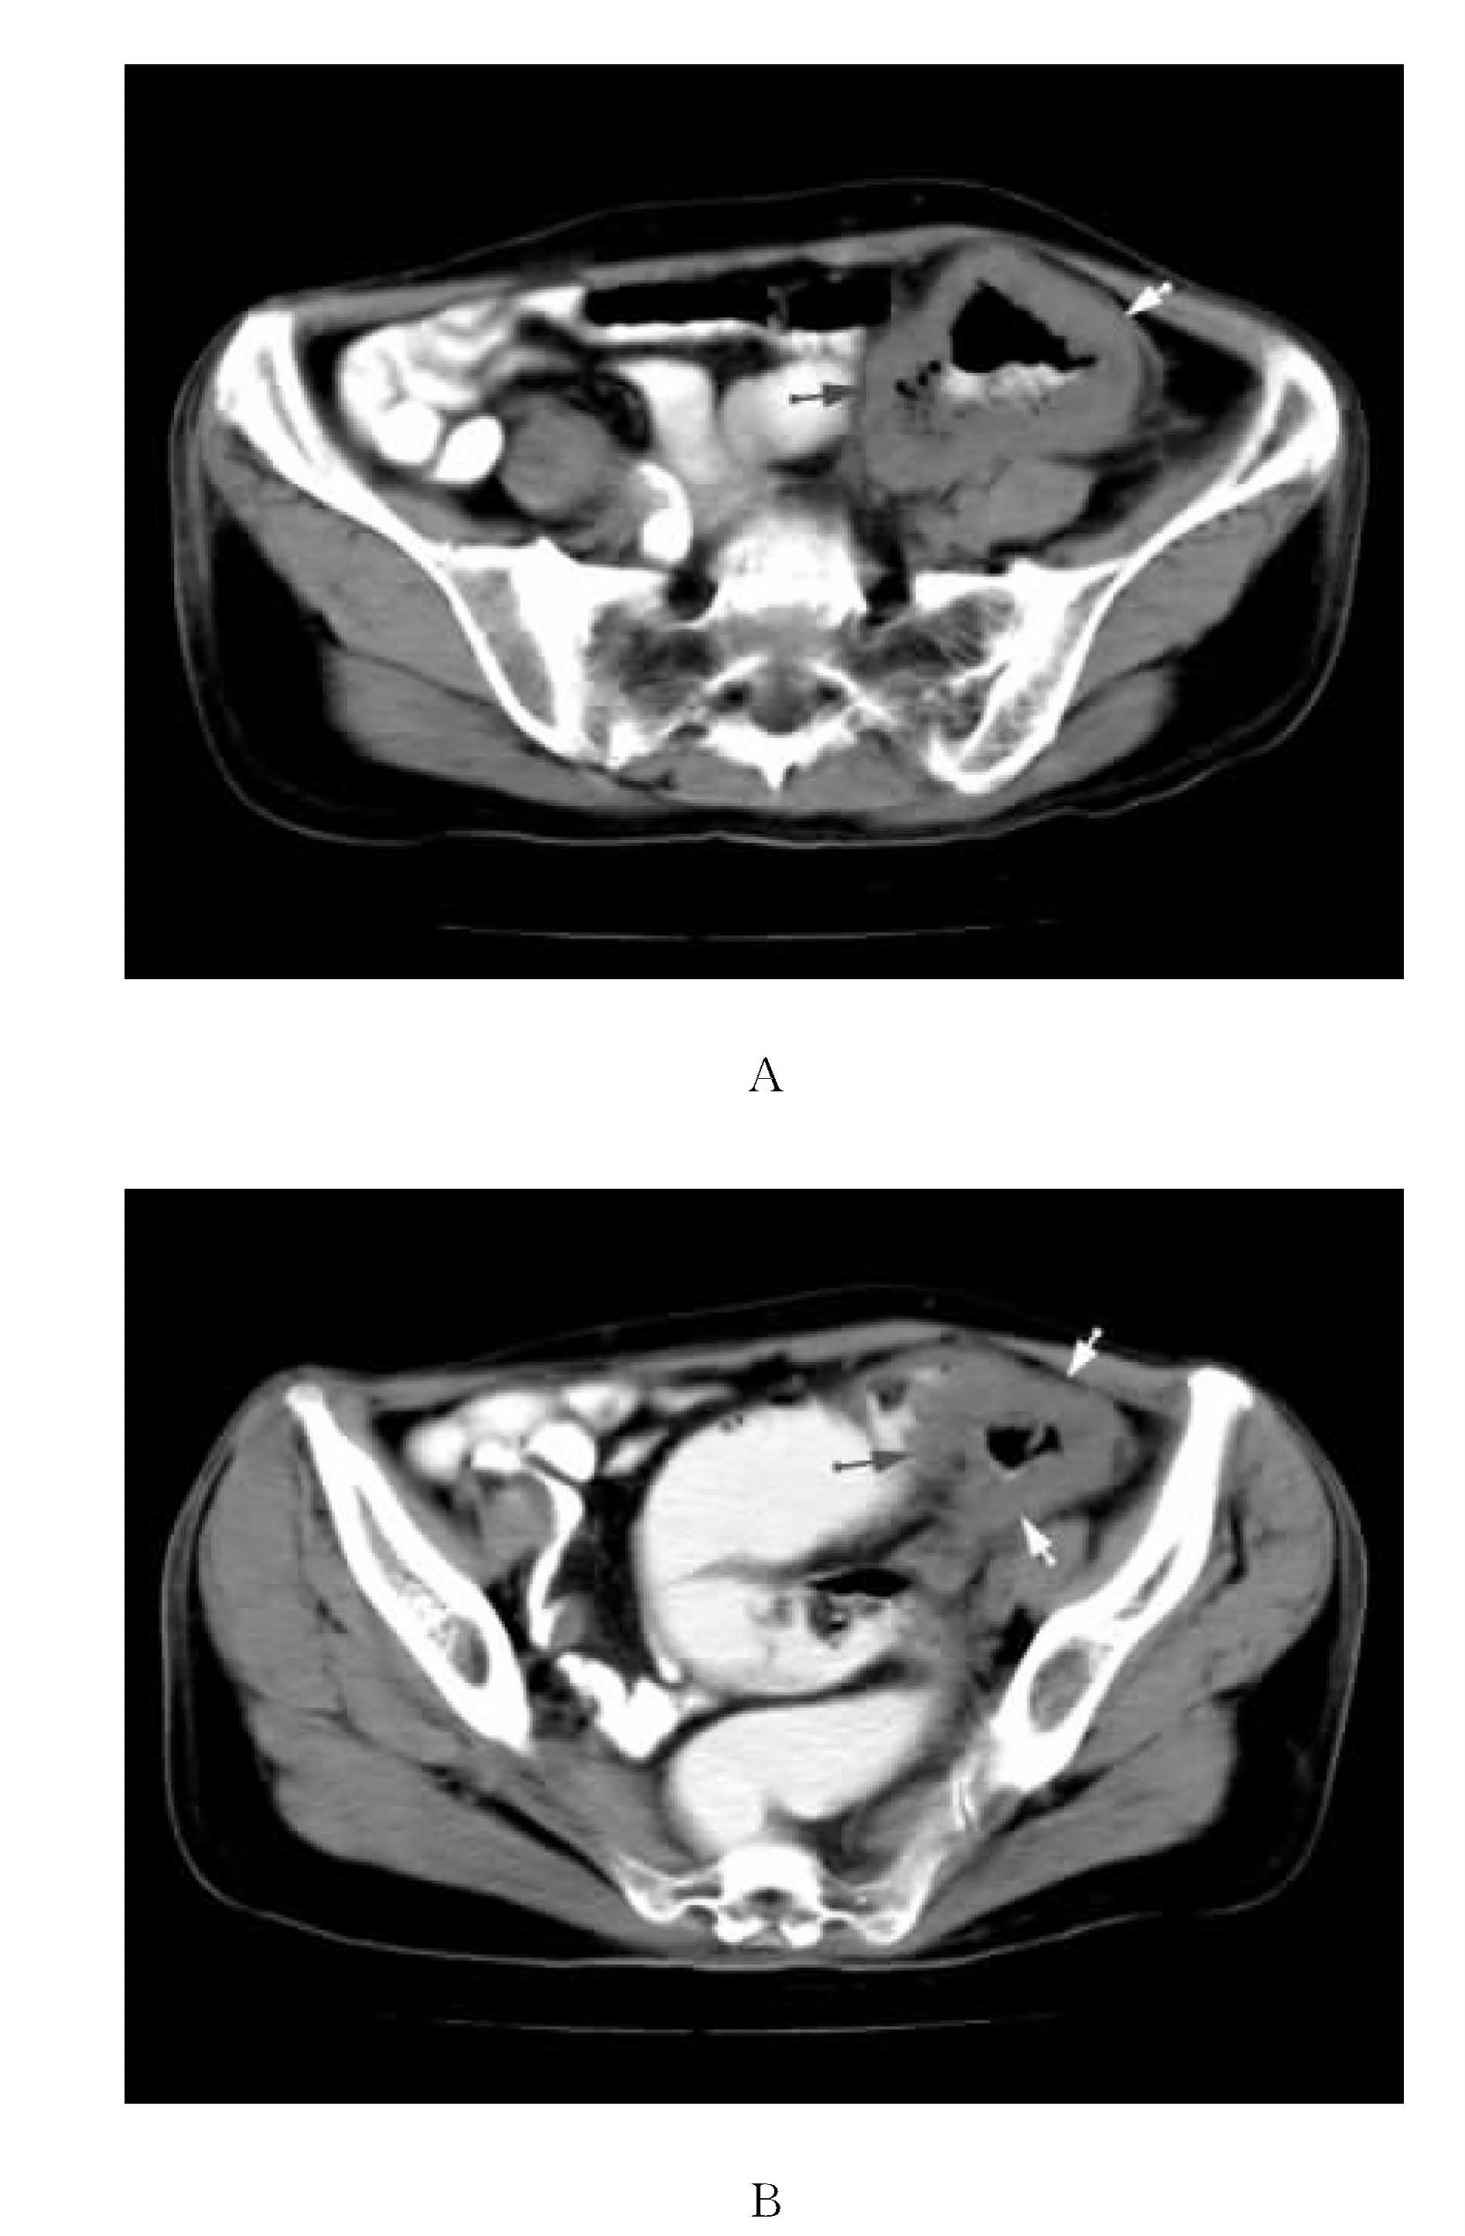
\includegraphics[width=.7\textwidth,height=\textheight,keepaspectratio]{./images/Image00365.jpg}
 \captionsetup{justification=centering}
 \caption{乙状结肠癌\\{\small A、B为同一患者,乙状结肠壁显著增厚,局部形成不规则软组织肿块}}
 \label{fig17-13}
  \end{figure} 

\textbf{【鉴别诊断】}
结肠癌应与其他恶性肿瘤如淋巴瘤、肉瘤区别。更重要的是与良性病变如憩室炎、阑尾炎症、异物穿孔鉴别。但以下表现高度提示为恶性肿瘤性病变:①局限性、分叶状软组织肿块,伴周围浸润性病变;②肠壁偏心性增厚>2cm;③增强扫描病灶明显强化;④合并有局部和(或)远处转移性病灶。

\subsection{直肠癌}

本病约占全身恶性肿瘤的15%,在男性仅次于胃癌,女性仅次于宫颈癌。80%~90%发生于直肠下2/3处,距肛缘10cm以内。

\textbf{【病理】}
多为腺癌,鳞状上皮细胞癌少见。大体病理亦可分为增殖型、浸润型、溃疡型、黏液型(又称胶样癌)。转移途径有直接浸润、淋巴转移和血行转移。

\textbf{【临床表现】}
早期多无明显症状。中晚期表现为轻重不一的局部刺激症状,如便意感、大便次数增多、里急后重、黏液便或黏液脓血便等,有些伴有贫血和恶液质;此期还可见大便变扁、变细。肿瘤侵及局部骶神经产生局部剧烈疼痛,侵及其他脏器有相应的症状和体征。

\textbf{【CT表现】}
①肠腔内实质性肿块:大小不一,常为1~10cm,边缘不规则。<5cm者密度均匀,与邻近肌肉密度相近或略高;>5cm者可有坏死而密度不均。②肠壁局限性或环状增厚:早期不明显,常为局限性,但肠壁厚度多>6mm(须充分扩张)。③肠腔环形或不对称狭窄:形态不规则、狭窄程度不一(图\ref{fig17-14})。④癌肿向肠壁周围浸润:浆膜面模糊毛糙、肠周脂肪密度升高,有时可见条索状软组织影,但不具特异性,也可见于炎性病变。如有肠外壁结节,则可肯定肠周浸润。⑤邻近组织和脏器受侵:如直肠周围肌肉、前列腺、阴道、输尿管、盆腔等。只有当这些邻近结构被原发癌肿包围、内部出现异常肿块或体积显著增大和密度改变时,才能肯定受侵。⑥淋巴结增大。⑦肝转移:不如结肠癌常见,多为小而多发,孤立转移常见。⑧癌性穿孔。

\begin{figure}[!htbp]
 \centering
 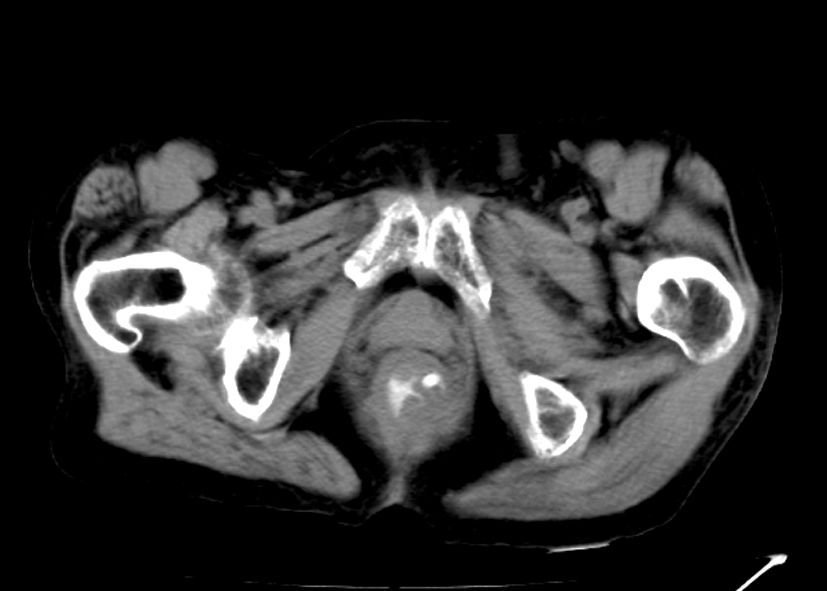
\includegraphics[width=.7\textwidth,height=\textheight,keepaspectratio]{./images/Image00366.jpg}
 \captionsetup{justification=centering}
 \caption{直肠癌\\{\small 直肠壁显著增厚,肠腔狭窄,肠壁边缘毛糙,肛提肌受侵}}
 \label{fig17-14}
  \end{figure} 

\subsection{大肠恶性淋巴瘤}

胃肠道是原发性结外NHL最常见的累及部位,约占37%。胃是最常见的部位约占50%,其次是小肠,而结肠和食管较少见。结肠病变通常侵犯盲肠和直肠。

\textbf{【病理】}
肿瘤起源于结肠的黏膜层和黏膜下层的淋巴组织,通常为非何杰金淋巴瘤(NHL),很少为何杰金淋巴瘤。肿瘤表现为突向肠腔内外的肿块,也可表现为从黏膜下到浆膜面肠壁的纵向浸润,并且常常伴有肠系膜淋巴结肿大。

\textbf{【临床表现】}
多见于50~60岁。常见有厌食和体重下降、下腹部绞痛,还有便血和腹泻、梗阻、穿孔和肠套叠等,常触及肿块。

\textbf{【CT表现】}
其基本的表现为肠壁增厚,厚度多>5cm,可达7~12cm。国内有学者将其分为3型:①局灶性肿块型:表现为肠道局部肠腔内或肠腔外的软组织肿块,肠管外形正常或消失;②节段性环形浸润型:受侵的肠段长短不一,但仍表现为肠壁的环形增厚,对称或稍不对称,局部尚保持肠道外形;③弥漫浸润型:呈节段性多发病变,累及大肠的全部或大部。

此外,当肿瘤侵及固有层内自主神经丛时,导致肠壁肌张力下降,引起管腔的扩张,表现为一特殊的征象即动脉瘤样扩张。亦可沿肠系膜浸润出现脂肪层密度增高、肠系膜增厚和条索影;肠系膜和腹膜后的淋巴结也可显著增大。

\textbf{【鉴别诊断】}
以下几点有助于与结肠癌鉴别。①淋巴瘤累及肠段较长,肠壁较厚,但由于病变区缺乏纤维结缔组织反应增生,使其肠腔变窄不明显,一般无梗阻表现;而大肠癌则相对较局限,常伴狭窄及梗阻。②盲肠淋巴瘤常直接累及回肠末端;而大肠癌少见。③淋巴瘤受累肠段周围脂肪界限清晰,很少直接向周围脂肪浸润;而大肠癌则常通过浆膜面直接向周围浸润。④淋巴瘤常不伴溃疡,少数有浅表溃疡,溃疡边缘平滑;而大肠癌常伴局限较大的边缘不规则的溃疡。⑤淋巴瘤可表现为多发弥漫浸润;而大肠癌相对较少。⑥淋巴瘤常表现为密度均一的肿块;而大肠癌较大的肿块常伴有缺血坏死的低密度区,且大肠癌强化明显高于淋巴瘤。

如在以上几点的基础上,同时发现明显的腹部淋巴结增大及肝、脾大,则进一步提示淋巴瘤的诊断。

\section{阑尾疾病}

\subsection{正常阑尾}

婴儿阑尾位于盲肠尖端;在发育中盲肠呈偏心性生长,成人的阑尾基底部则位于盲肠内后侧回盲瓣下方2.5cm处;外形从漏斗状(婴儿期)变成蚯蚓状盲管。其长短、粗细不一,长5~7cm,最长可达20cm,或短至1cm;直径约6mm。方向不定。

阑尾尖端的指向有很大不同,约2/3位于盲肠后,其余多位于内下部。常见有5种:①回肠下位(盆腔位);②盲肠后位(结肠后位);③盲肠下位(髂窝位);④回盲前位;⑤回盲后位。此外,还有少见的高位阑尾(肝脏下位)、低位阑尾(降至小骨盆内)、腰部阑尾(盲肠后腹膜外阑尾)及位于左髂窝或腹腔中部的阑尾。

\textbf{【CT表现】}
阑尾呈薄壁的管腔,周围是肠系膜脂肪影,正常成人管径<6mm,儿童<8mm。口服或灌肠造影剂,常可使阑尾充盈。

\subsection{急性阑尾炎}

\textbf{【病因病理】}
本病大多数由于阑尾管腔机械性阻塞或痉挛导致的功能性阻塞和细菌感染而引起。有3种病理类型:①急性单纯型:为早期阑尾炎,阑尾黏膜或黏膜下层发生炎性水肿,阑尾轻度肿胀;②急性蜂窝组织炎型:又称急性化脓性阑尾炎。炎症向深层发展达肌层和浆膜层,阑尾高度肿胀,并可扩展至阑尾周围引起阑尾周围炎及局限性腹膜炎;③急性坏疽型:炎症进展使阑尾坏死,常导致穿孔,引起阑尾周围脓肿或弥漫性腹膜炎。

\textbf{【临床表现】}
特点是阵发性、转移性右下腹痛,麦氏点压痛、反跳痛,可伴发热及胃肠道症状如恶心、呕吐。腹膜炎时可有畏寒、高热及麻痹性肠梗阻。部分患者临床表现不典型,其中年龄大及体质弱是主要原因。

\textbf{【CT表现】}

1.直接征象:①阑尾肿大增粗(成人直径>6mm,儿童>8mm)和阑尾管壁增厚(>2mm),密度接近或略高于邻近的肌肉,边缘模糊,与周围的炎症分界不清。②阑尾的管状结构消失,有时增厚的阑尾壁表现为不同密度分层的“同心圆”样结构。③部分病例伴有一个或多个阑尾结石,但单凭这一征象仍有假阳性的可能。

2.间接征象:①箭头征:盲肠顶部管壁增厚,阑尾开口居于其中间部,对比剂在闭塞的阑尾开口上方形成漏斗状集聚,在CT上对比剂呈箭头状称为箭头征。国外有学者认为,若见到此征象特异性达100%。末端回肠壁亦可增厚。②阑尾盲肠周围炎性改变:约70%出现,邻近脂肪间隙模糊、密度增加,出现密度增高的条索影;盲肠壁局部增厚,甚至引起右结肠侧筋膜的增厚和结节样隆起;阑尾四周可有少量液体渗出;当炎症向周围蔓延可致盲肠与右侧腰大肌之间的脂肪间隙模糊;亦可形成阑尾区炎性软组织肿块;还可见阑尾起始部4cm范围内淋巴结肿大。

3.阑尾周围脓肿:为另一较常见的表现,由阑尾穿孔所致。直径多为2~10cm,常位于右髂窝区结肠近端、盆腔、升结肠后和右结肠旁沟。

4.穿孔性阑尾炎的特点:国内有学者报道,蜂窝组织炎、腹膜腔脓肿、阑尾壁强化伴缺损和阑尾周围积气是阑尾炎的直接征象,并对穿孔性阑尾炎的诊断有很高的特异性。穿孔性较非穿孔性阑尾肿大更著。间接征象中肠壁增厚、腹水、回肠壁强化、阑尾内积气,以及积气合并阑尾附近大肠炎,穿孔性亦明显高于非穿孔性。

总之,如发现阑尾周围有炎性改变、脓肿和结石,而没有发现异常的阑尾只能高度怀疑为急性阑尾炎;如同时显示异常增粗的阑尾可诊断为急性阑尾炎。

\subsection{慢性阑尾炎}

\textbf{【病因病理】}
本病可由急性阑尾炎转化而来,也可由于阑尾结石、异物、寄生虫等引起管腔梗阻与刺激而导致阑尾慢性感染。病理显示阑尾壁纤维肉芽组织增生,使之增厚、管腔狭窄甚至闭塞,阑尾周围粘连而扭曲等。管腔狭窄局限者,在其远端常有粪石存留。病变的反复发作迁延,常伴慢性盲肠周围炎及脓肿形成。

\textbf{【临床表现】}
主要症状为右下腹痛,呈间歇性或持续性隐痛。体检右下腹有局限压痛。

\textbf{【CT表现】}
主要是阑尾及盲肠周围的慢性炎症表现。阑尾可有不同程度的增粗,阑尾腔闭塞,阑尾边缘毛糙;多伴有钙化或阑尾结石。慢性阑尾炎反复发作形成的脓肿包块,可与盲肠周围的筋膜、腹膜粘连,使之增厚、密度增加;包块还可对周围器官产生压迫,使其变形和移位。

\subsection{阑尾黏液囊肿}

\textbf{【病因病理】}
本病多继发于阑尾慢性炎症。是由于阑尾腔的闭塞,造成黏液的异常积聚,导致阑尾腔的扩大而形成的囊性肿块。早期黏液稀薄,以后因水分吸收而呈胶冻状。可合并囊腺癌。还有人将其分为3类:①单纯潴留囊肿;②黏液囊腺瘤;③黏液囊腺癌。但似欠合理。

\textbf{【临床表现】}
缺乏特异性,20%无症状。主要症状类似阑尾炎,有右下腹痛、压痛,可触及包块,极少数可引起肠套叠。

\textbf{【CT表现】}
典型表现为右下腹阑尾区的囊性肿块影,呈局限性的圆形或肾形软组织肿块,其基底部与盲肠相连。囊肿大小不一,其内容物从水样至软组织密度,CT值约0~30Hu。囊壁薄,边缘光整。囊壁内可有点状或弧形钙化,有时可见囊内分隔。肿块套入盲肠内呈同心圆状表现。黏液球囊肿是本病的一种特殊类型,阑尾腔内充盈着许多固态的半透明的球状小体,这些小体可出现钙化,并随体位改变而移位。

\textbf{【鉴别诊断】}
①黏液囊肿的周围一般不伴炎症或脓肿,有助于与急性阑尾炎鉴别。②当囊性肿块内有气体时,应注意区分是囊肿合并感染还是脓肿。囊壁呈壳状钙化且周围缺乏炎症提示黏液囊肿可能性大;而脓肿可出现于多个部位,壁较厚且厚薄不均,钙化多呈点状,周围多有炎症,有时可见阑尾结石。

\subsection{阑尾黏液囊腺癌}

本病发生率极低,约占阑尾疾病的1.0%~1.5%。多手术偶然发现。

\textbf{【病理】}
表现为腺上皮的不典型增生,腺瘤可致阑尾腔阻塞,黏液在阑尾腔内潴留,并可穿透到浆膜,引起腹膜种植形成腹膜假性黏液瘤,但不发生淋巴和血行转移。有时可伴卵巢黏液性囊腺癌。

\textbf{【临床表现】}
酷似慢性阑尾炎。无急性阑尾炎的症状和体征,局部可触及腹块,轻压胀痛,无恶心、呕吐,无腹泻、便血。

\textbf{【CT表现】}
右下腹阑尾区局限性低密度囊性肿块,其基底与盲肠相连,直径多较大(图\ref{fig17-15})。囊壁不规则并可出现壁结节,结节密度从近水样至软组织密度。增强扫描囊壁和结节呈不均匀强化。形成腹膜假性黏液瘤(CT值5~20Hu)可显示腹水,肝缘、腹壁、肠袢可以见到腹膜种植所致的压迹,肠间距增宽、肠袢分离。黏蛋白结节可出现钙化。

\begin{figure}[!htbp]
 \centering
 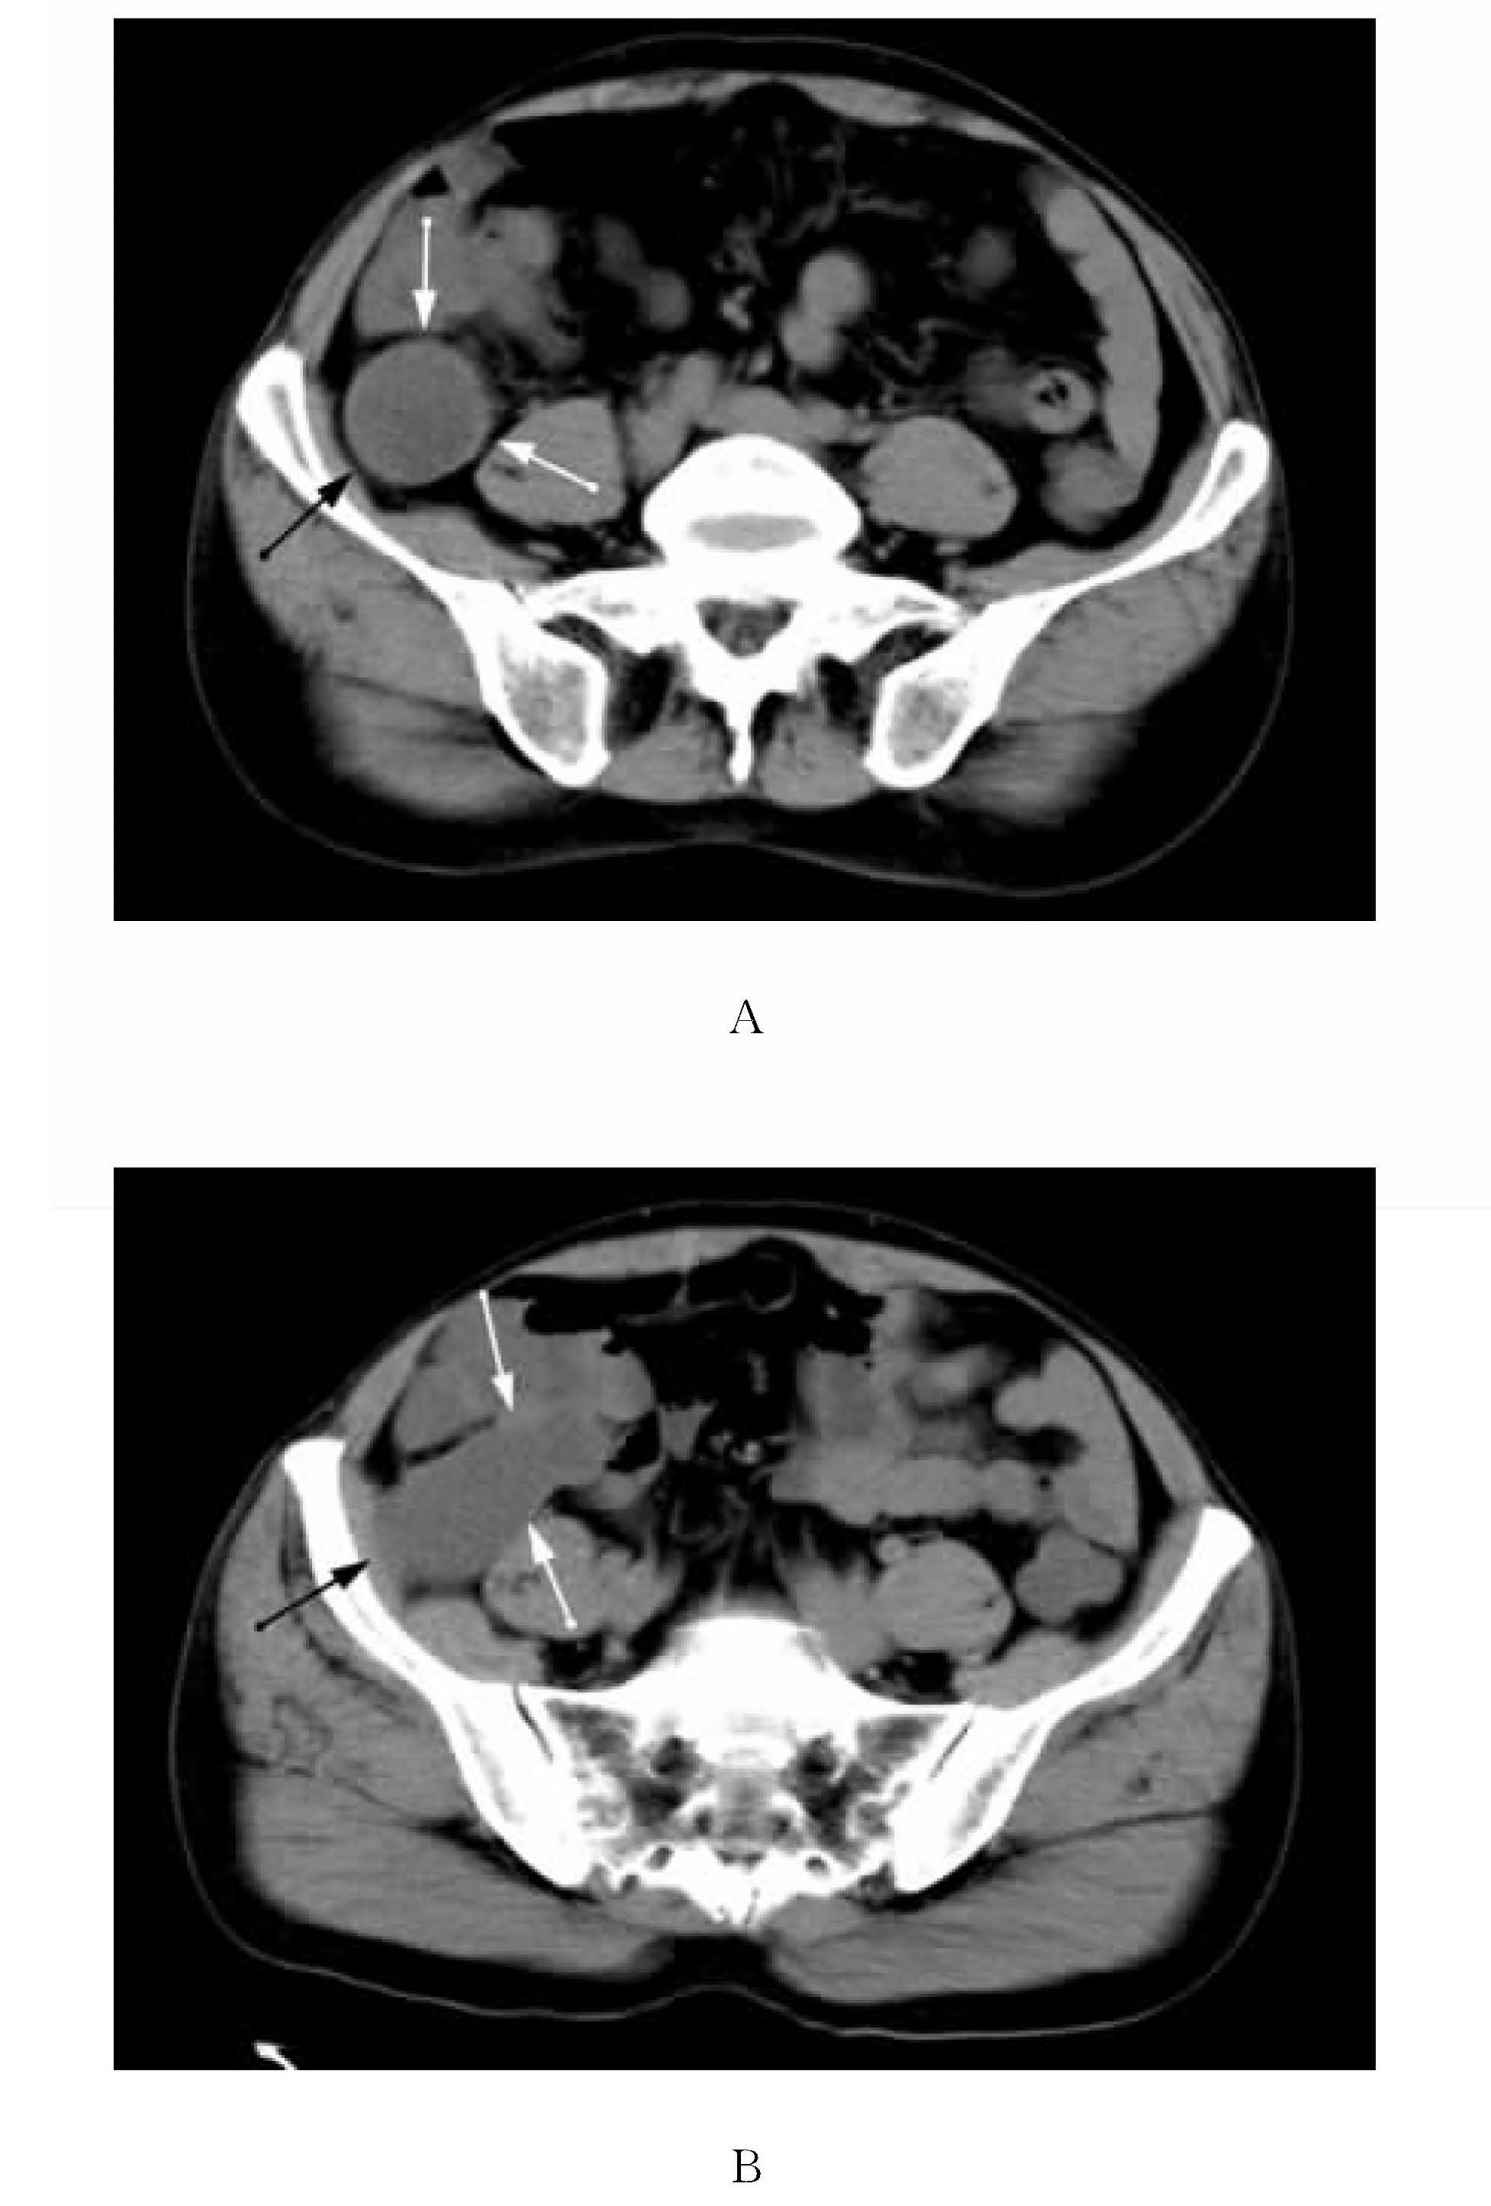
\includegraphics[width=.7\textwidth,height=\textheight,keepaspectratio]{./images/Image00367.jpg}
 \captionsetup{justification=centering}
 \caption{阑尾黏液囊肿\\{\small A、B为同一患者,右侧髂窝区囊状水样低密度灶,边缘光滑锐利,其下端与回盲部关系密切}}
 \label{fig17-15}
  \end{figure} 

\textbf{【鉴别诊断】}
病灶如无明显壁结节和腹膜假性黏液瘤,则与黏液囊肿或囊腺瘤难以鉴别。

\subsection{阑尾类癌}

本病又称嗜银细胞瘤。约有30%~45%的胃肠道类癌发生于阑尾,是类癌发生率最高的部位。占阑尾肿瘤的90%左右。

\textbf{【病理】}
起源于阑尾(胃肠)黏膜腺体的嗜银细胞,生长缓慢,大小多<2cm。颜色淡黄,质地坚实。瘤细胞较小,细胞内含有5-羟色胺颗粒。恶性程度较低,3%发生转移,8%可侵及肌层。

\textbf{【临床表现】}
可发生于任何年龄,以30~50岁多见。阑尾类癌多无明显的临床症状而偶然发现。肿瘤阻塞管腔时易诱发阑尾炎而出现相应症状。极少数出现类癌综合征,如皮肤潮红、腹泻、哮喘、心瓣膜病等。

\textbf{【CT表现】}
主要表现为阑尾区的软组织密度肿块,70%在阑尾的远段,20%在中段,10%在基底部。瘤体较大时可在回肠末段和盲肠产生压迹。基底部者阻塞阑尾腔,可产生阑尾炎的表现。合并肝脏或淋巴结等转移可出现相应表现。

\section{肠梗阻}

\subsection{概述}

肠梗阻是指肠内容物不能正常运行或通过发生障碍的状态。

\textbf{【分类】}
①按梗阻的原因不同分为机械性肠梗阻、动力性肠梗阻、血运性肠梗阻;②按有无肠壁的血运障碍又可分为单纯性肠梗阻和绞窄性肠梗阻;③按梗阻部位的高低分为高位肠梗阻和低位肠梗阻。

\textbf{【病因】}

1.机械性肠梗阻:病因复杂多样,如肠粘连、原发性或继发性肿瘤、克隆病、血管性病变、寄生虫、大胆石、粪块、腹部疝、慢性结肠憩室炎、肠套叠、肠扭转等。

2.麻痹性肠梗阻:常见原因有腹部手术、创伤、炎症、铅中毒等。

3.血管性肠梗阻:主要为肠系膜动脉或静脉的血栓形成或栓塞,可发生于肠系膜血管的任何部位,但以肠系膜上动脉、静脉的主干或分支好发。

\textbf{【病理】}
不论何类肠梗阻均有内容物通过受阻,肠壁吸收气体和液体的能力减弱以至消失,甚至分泌更多的液体。于是形成肠内潴积多量的气体和液体,将肠腔撑大。

\textbf{【CT表现】}
基本CT征象为肠管扩大,其内可见液-气平面;也可完全被液体所充盈,肠壁变薄。扩大充气的小肠、结肠呈连续的管状。小肠宽约3cm以上,左半结肠常达5cm以上,右侧结肠常达7cm以上。梗阻远端肠管明显塌陷,梗阻远、近端肠管直径的明显差异是诊断肠梗阻非常有价值的诊断征象。

1.机械性肠梗阻:诊断时应注意:①肠粘连占肠梗阻病例的1/3。有时CT可显示粘连的索条、部位。当在“移行带”未发现明确病变时,应考虑肠粘连可能。②肿瘤引起的肠梗阻,一般可以准确地显示肿瘤的发生部位及其对周围组织器官的侵袭范围。③胆石性肠梗阻可见下腹部异位钙化的胆石。④还应考虑以下问题:腹内、腹外疝的存在与否;是否存在两种以上的病因;有无两处以上的梗阻;是否合并先天性肠管畸形等。

机械性肠梗阻程度的判断:①完全性肠梗阻:“移行带”移行非常突然或明显,“移行带”以远无对比剂通过。小肠完全性肠梗阻,结肠常塌陷,含十分少量或不含气、液体(图\ref{fig17-16})。②部分性肠梗阻:“移行带”移行缓慢或不明显,“移行带”以远的肠管部不完全塌陷。小肠梗阻时结肠内含中量气体或液体,24小时延迟扫描可见口服对比剂通过。

\begin{figure}[!htbp]
 \centering
 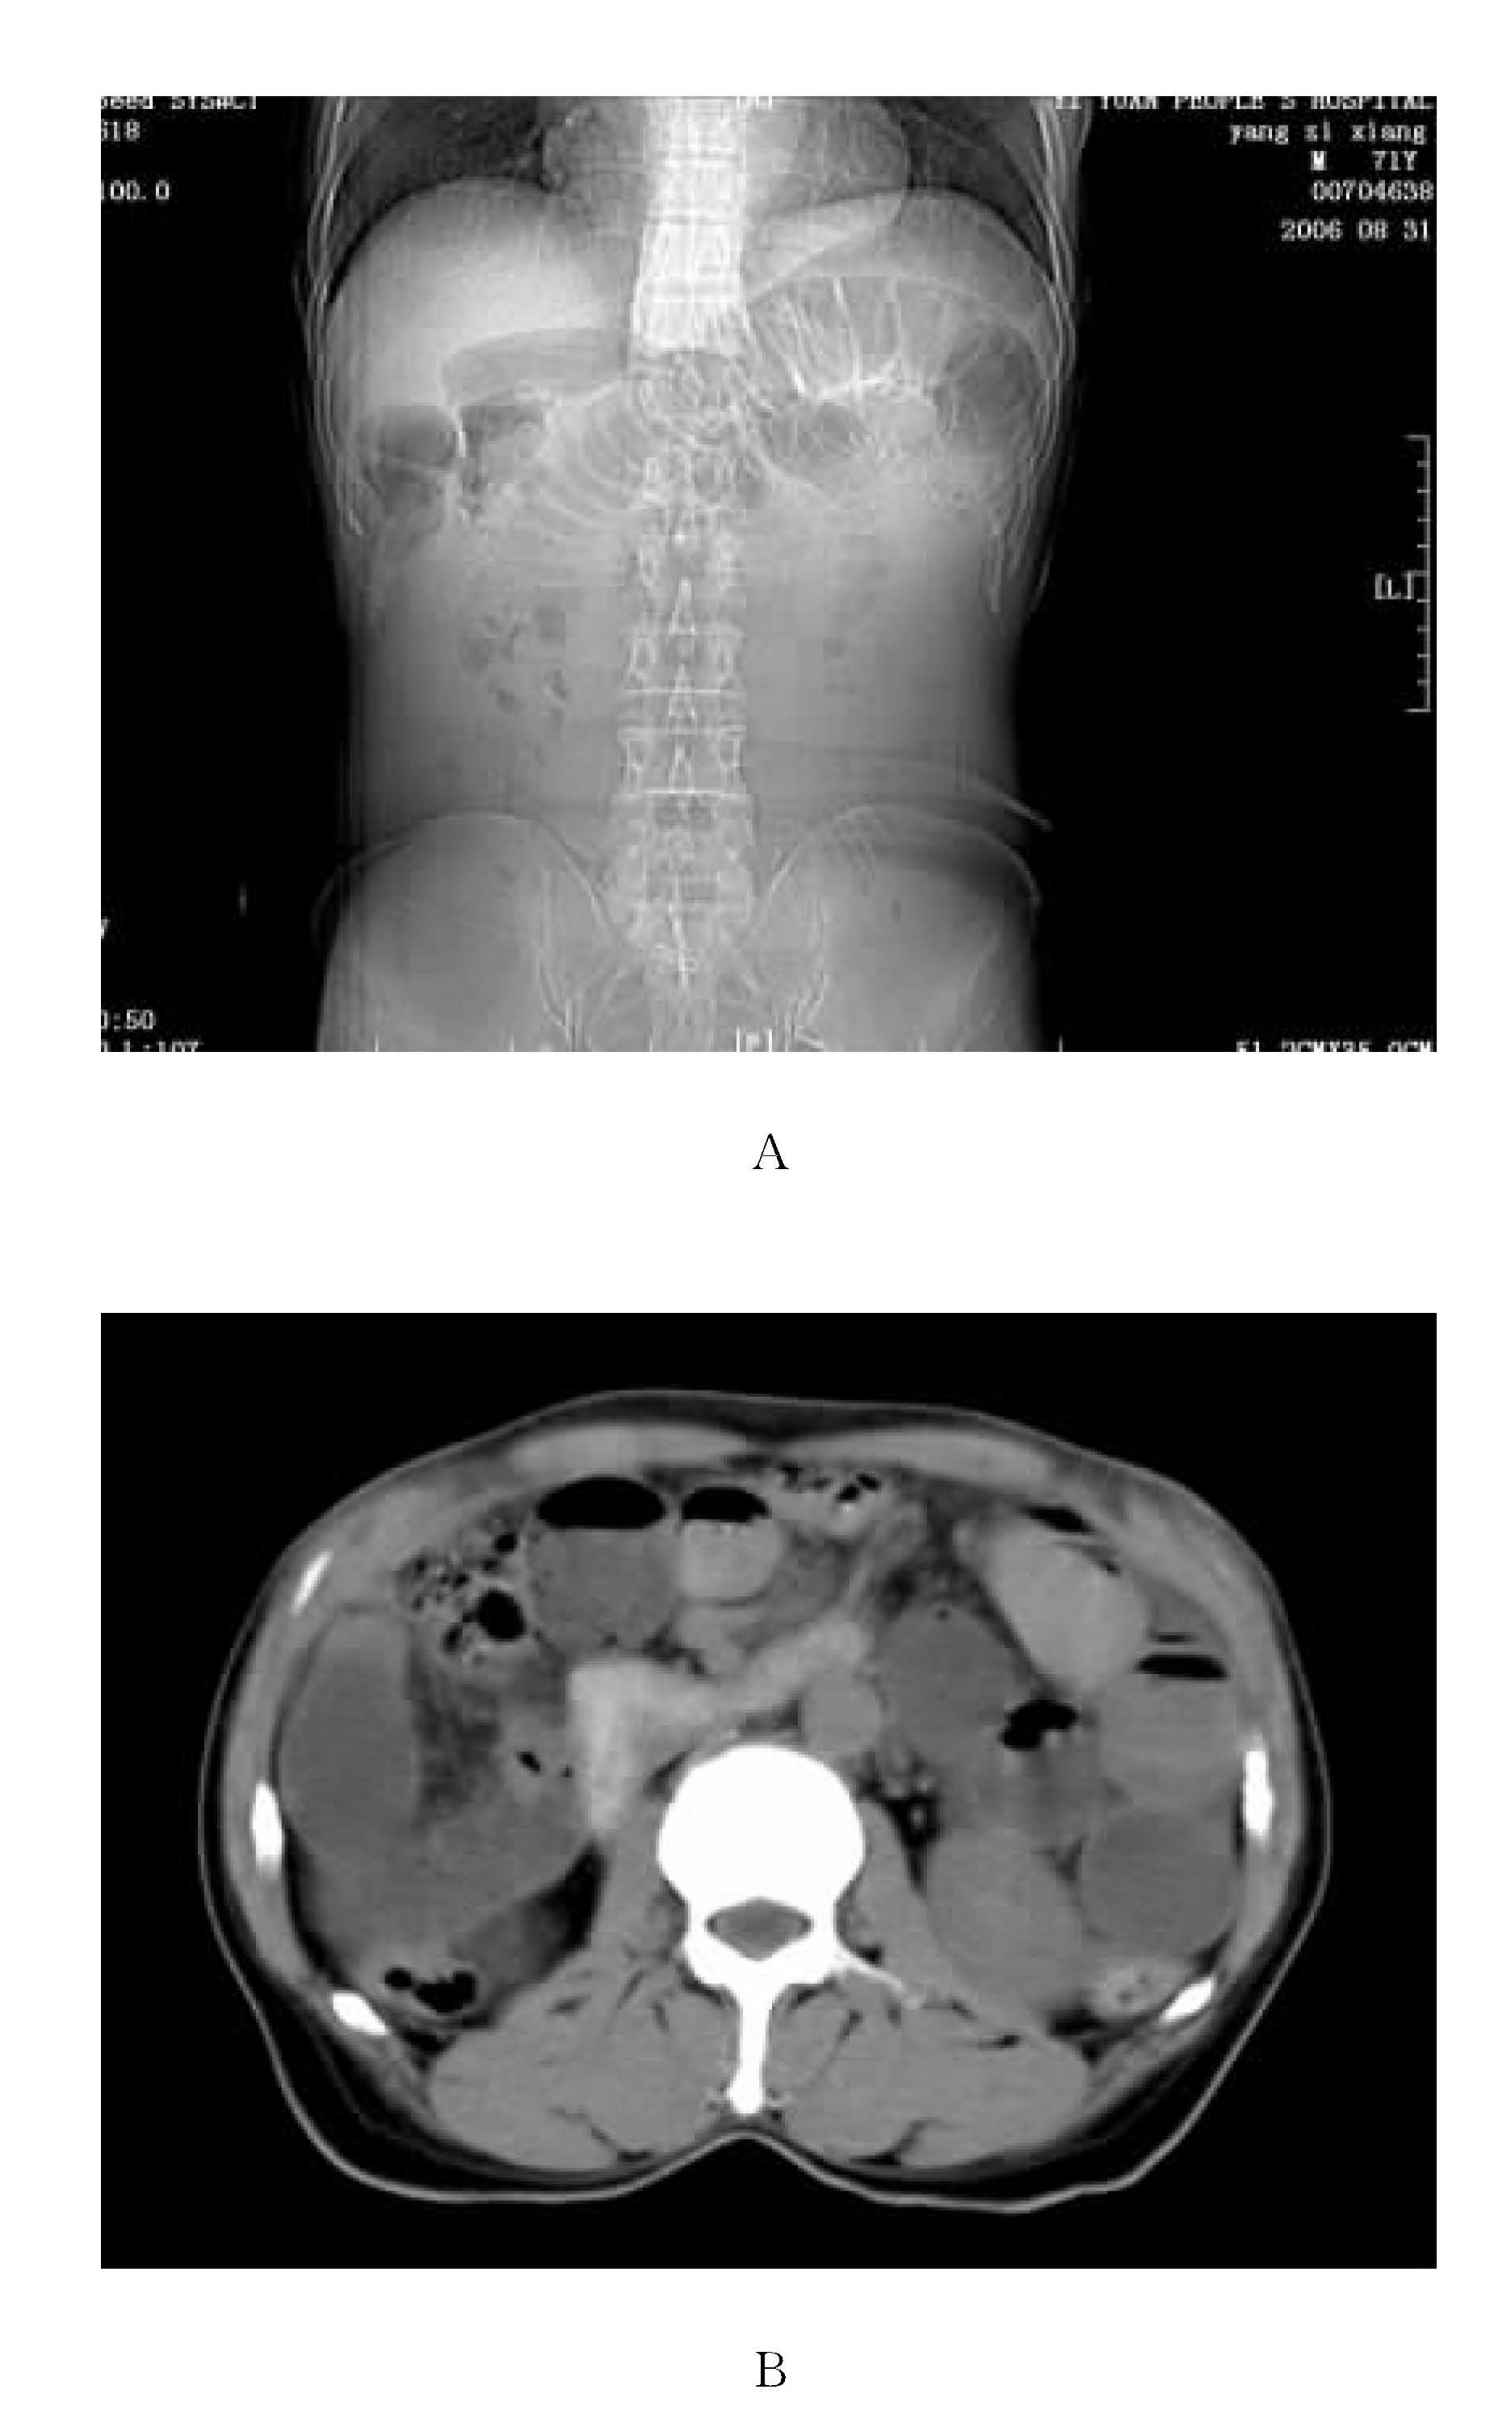
\includegraphics[width=.7\textwidth,height=\textheight,keepaspectratio]{./images/Image00368.jpg}
 \captionsetup{justification=centering}
 \caption{机械性肠梗阻(小肠)\\{\small A、B为同一患者,A示上腹部小肠(空肠)呈管状扩张,其黏膜皱襞呈弹簧状;B示许多小肠扩张积液,并有液气平面}}
 \label{fig17-16}
  \end{figure} 

2.麻痹性肠梗阻:与单纯性肠梗阻相反,麻痹性肠梗阻的CT表现为成比例的小肠及结肠扩张,而无“移行带”的出现;延迟12~24小时扫描结肠充气、扩张、积液或有口服对比剂的出现。CT有时可显示其病因(如炎症)的相应表现。但某些病例可误为机械性梗阻。

有时麻痹性与机械性肠梗阻可合并存在。例如小肠机械性肠梗阻引起腹膜炎,进而可导致麻痹性肠郁张,可表现为既有“移行带”的出现,又有结肠轻度扩张的表现。

3.血管性肠梗阻:除可见结肠脾曲以前的小肠、结肠麻痹性扩张外,还可见肠缺血的相应CT表现(详见本章第六节)。增强扫描可发现肠系膜动脉或静脉的阻塞、气栓等。

\subsection{单纯机械性肠梗阻}

\textbf{【病因病理】}
常见原因小肠为肠粘连、粘连索带压迫、小肠炎性狭窄和肿瘤。大肠梗阻部位大多数在左半结肠,尤以乙状结肠和直肠更为多见,多为肿瘤和炎性狭窄。小肠阻塞之后,其内容物通过受障,所以阻塞以上肠曲扩大,阻塞以下肠曲空虚、萎陷。肠曲扩大是从靠近梗阻部位的近端开始,越向上端扩大越轻。大肠阻塞之后,则扩张的大肠横径以盲肠为最大,向梗阻点逐渐变小;但也有少数越近梗阻点扩大越显著。在梗阻程度严重、梗阻时间较久的情况下,可在靠近梗阻点处引起血供障碍,最后可发生坏死和穿孔。

\textbf{【临床表现】}
主要为肠绞痛,疼痛性质为阵发性锐痛,间歇期可没有腹痛或隐隐作痛,疼痛逐渐加重,还常伴有恶心、呕吐、便秘和肛门不排气。体检可见腹胀、肠型;有时有压痛、无反跳痛;肠鸣音亢进。大肠单纯性梗阻则便秘较为突出,而恶心、呕吐常为次要症状。

\textbf{【CT表现】}

1.较特异的征象是扩张的近侧肠管与塌陷或正常管径的远侧肠管之间“移行带”的出现。但国外学者提出,在结肠段以此征象作为诊断机械性肠梗阻的依据并不十分可靠,并认为应重扫“移行带”寻找梗阻病变,如未发现梗阻病变则应考虑为麻痹性肠梗阻。

2.小肠粪便征:指扩张的小肠中出现气体与某种物质的混合物征象,类似结肠中的粪便表现,可能有助于诊断小肠梗阻。

3.连续性肠袢扩张和狭窄前的肠扩张:在诊断肠梗阻中亦有重要价值。前一征象是指“移行带”近侧所有肠管的扩张;后一征象为只位于“移行带”之前的那部分肠管的扩张。

此外,CT对胆石性肠梗阻的诊断有独到的价值。

\subsection{闭袢性肠梗阻}

本病是指一段肠管在其行程上两点被梗阻,且这两点彼此相近被同一原因所限制。

\textbf{【病因病理】}
多由肠袢沿肠系膜长轴旋转引起的肠扭转所致,也可由纤维束带的粘连、内疝等将一段肠管的两端收缩聚拢而形成闭袢。因多伴有梗阻肠袢的血供障碍,故有文献将闭袢性肠梗阻习惯称为绞窄性肠梗阻。有完全性和不完全性之分。完全性闭袢的近端梗阻点完全阻塞,阻塞以上的肠内容物不能进入闭袢;不完全性的近端梗阻点为部分阻塞,阻塞以上肠曲的气体和液体可进入闭袢。

\textbf{【临床表现】}
主要是腹痛、恶心、呕吐、便秘等。但常起病突然、腹痛为持续性或持续性腹痛伴阵发性加剧。有绞窄者常出现休克、腹膜刺激征和WBC升高等。

\textbf{【CT表现】}

1.梗阻受累肠管的表现:①当扫描层面通过闭袢时,可表现为两个扩张的肠环,随层面逐渐靠近闭袢根部,可见两个相邻肠环的距离逐渐接近。②当闭袢与扫描层面并行时,可表现为一扩张的U形肠袢,肠管呈相似程度扩张,肠腔内充满液体。

2.梗阻部位的表现:①当扫描层面通过闭袢根部时,可见肠管的变形,肠扭转时则表现为一个三角形的软组织密度影。②扫描层面通过闭袢的输入与输出端时,则表现为相邻的两个萎陷的肠环。③当肠扭转闭袢的输入或输出段肠管的长轴与CT扫描层面平行时,由于扭转使输入段逐渐变细,输出段由细变粗,梗阻处表现为“鸟嘴征”。

3.受累肠系膜的表现:肠系膜血管拉长或增厚,并示扩张肠袢的肠系膜血管呈放射状向闭袢的根部聚拢。在肠扭转时,聚拢的肠系膜血管可形成“漩涡征”,中心软组织密度为上一级的肠系膜动脉,周围为伸展扩张的小血管。

此外,一般闭袢内充满液体,而其近侧的肠袢内则充有大量气体。无上述征象者不可完全排除闭袢性肠梗阻。

\subsection{绞窄性肠梗阻}

这种梗阻由于肠系膜血管发生狭窄,致使血液循环发生障碍,引起某受累段肠管坏死(而非单纯梗阻的梗阻点附近的缺血坏死)。一般见于闭袢性肠梗阻。

\textbf{【临床表现】}
除表现为肠绞痛、恶心、呕吐、便秘等。有以下特点:①常起病突然,一开始就剧烈腹痛;②腹痛为持续性或持续性腹痛伴阵发性加剧;③起病后立即就有反射性呕吐;④常出现休克症状;⑤出现腹膜刺激征;⑥肠鸣音可以减少;⑦化验可见周围血白细胞和中性粒细胞升高。

\textbf{【CT表现】}
肠缺血可能出现以下CT征象:①肠壁环形增厚,厚度约0.5~1.0cm,可呈节段性分布。并可出现分层现象表现为“双晕征”或“靶征”。②增强扫描时,病变处肠壁不强化或强化明显减弱;当延迟扫描时,正常肠壁强化现象已消失,而病变处肠壁出现强化,随时间的延长可达正常肠壁的强化程度。③肠扭转时可见光滑的鸟嘴征,但因梗阻处肠壁的水肿增厚和肠系膜的充血、水肿,变为锯齿状鸟嘴征。④腹水的出现开始为少量,逐渐变为大量。⑤肠系膜血管床弥漫性模糊、充血,表现为肠系膜密度增高、模糊呈云雾状,CT值上升可达-60~-40Hu。肠系膜血管逐渐变粗并呈放射状,由梗阻处向外放射。⑥肠壁出现梗死时,可见肠壁内积气,肠系膜静脉和门静脉内亦可见气体影;增强扫描有时可见肠系膜动、静脉血栓形成。

总之,多数文献强调,“靶征”、肠壁强化明显减弱和腹水是提示绞窄性肠梗阻的可靠征象。此外,不出现前述的征象不能完全排除肠绞窄。

\textbf{【鉴别诊断】}
绞窄性肠梗阻与肠系膜缺血的CT表现类似,但前者合并肠梗阻征象;后者则无肠梗阻表现而可出现血管闭塞的直接征象。

\subsection{成人肠套叠}

成人肠套叠少见,约占肠梗阻的1%。它与常见的儿童原发性肠套叠不同,多由器质性病变引起。

\textbf{【病因病理】}
成人继发性肠套叠的病因众多。①良性病变:有脂肪瘤、平滑肌瘤、血管瘤、神经纤维瘤、腺瘤样息肉、感染性病变、美克尔憩室、术后粘连及肠动力性病变等;②恶性病变:有转移癌、腺癌、类癌、淋巴瘤、平滑肌肉瘤等。总之,成人肠套叠以小肠多见,常由良性病变继发,且以脂肪瘤最常见;相对而言结肠型肠套叠则更多由恶性病变继发。

肠套叠由套入部与鞘部组成。套叠局部肠壁反折共分为3层,由内至外分别称内筒、中筒和外筒。内筒和中筒合称套入部,外筒又称为套鞘。外筒与中筒的反折部称为套叠颈部,中筒与内筒的反折部称为套叠头部。病理可分为3型:①回结肠型:回肠套入结肠内;②小肠型:小肠套入小肠;③结肠型:结肠套入结肠。

\textbf{【临床表现】}
成人肠套叠不一定有急腹症表现,多表现为慢性复杂性肠梗阻。主要表现为腹痛、腹部不适,急性者(病程3天以内者)为持续性腹痛、阵发性加剧,亚急性、慢性者(病程5天以上者)腹痛有缓解期。腹痛发作时可伴恶心、呕吐、便血和停止排气。还可触及腹部包块、发热等。

\textbf{【CT表现】}

1.靶征:是最常见的特征性表现,当扫描层面与套叠部位垂直时出现此征(图\ref{fig17-17})。它反映了套叠的各层肠壁、肠腔及肠系膜之间的解剖关系,外层为较薄的套鞘、内为套入部,以套入的肠系膜脂肪形成新月形或半环形的脂肪密度透亮区最具特征。靶块多呈圆形或类圆形,可见2~3层肠壁。但由于套叠长轴与CT扫描层面角度的不同,也可呈肾形、香蕉形或弹簧状和舌状肿块。

\begin{figure}[!htbp]
 \centering
 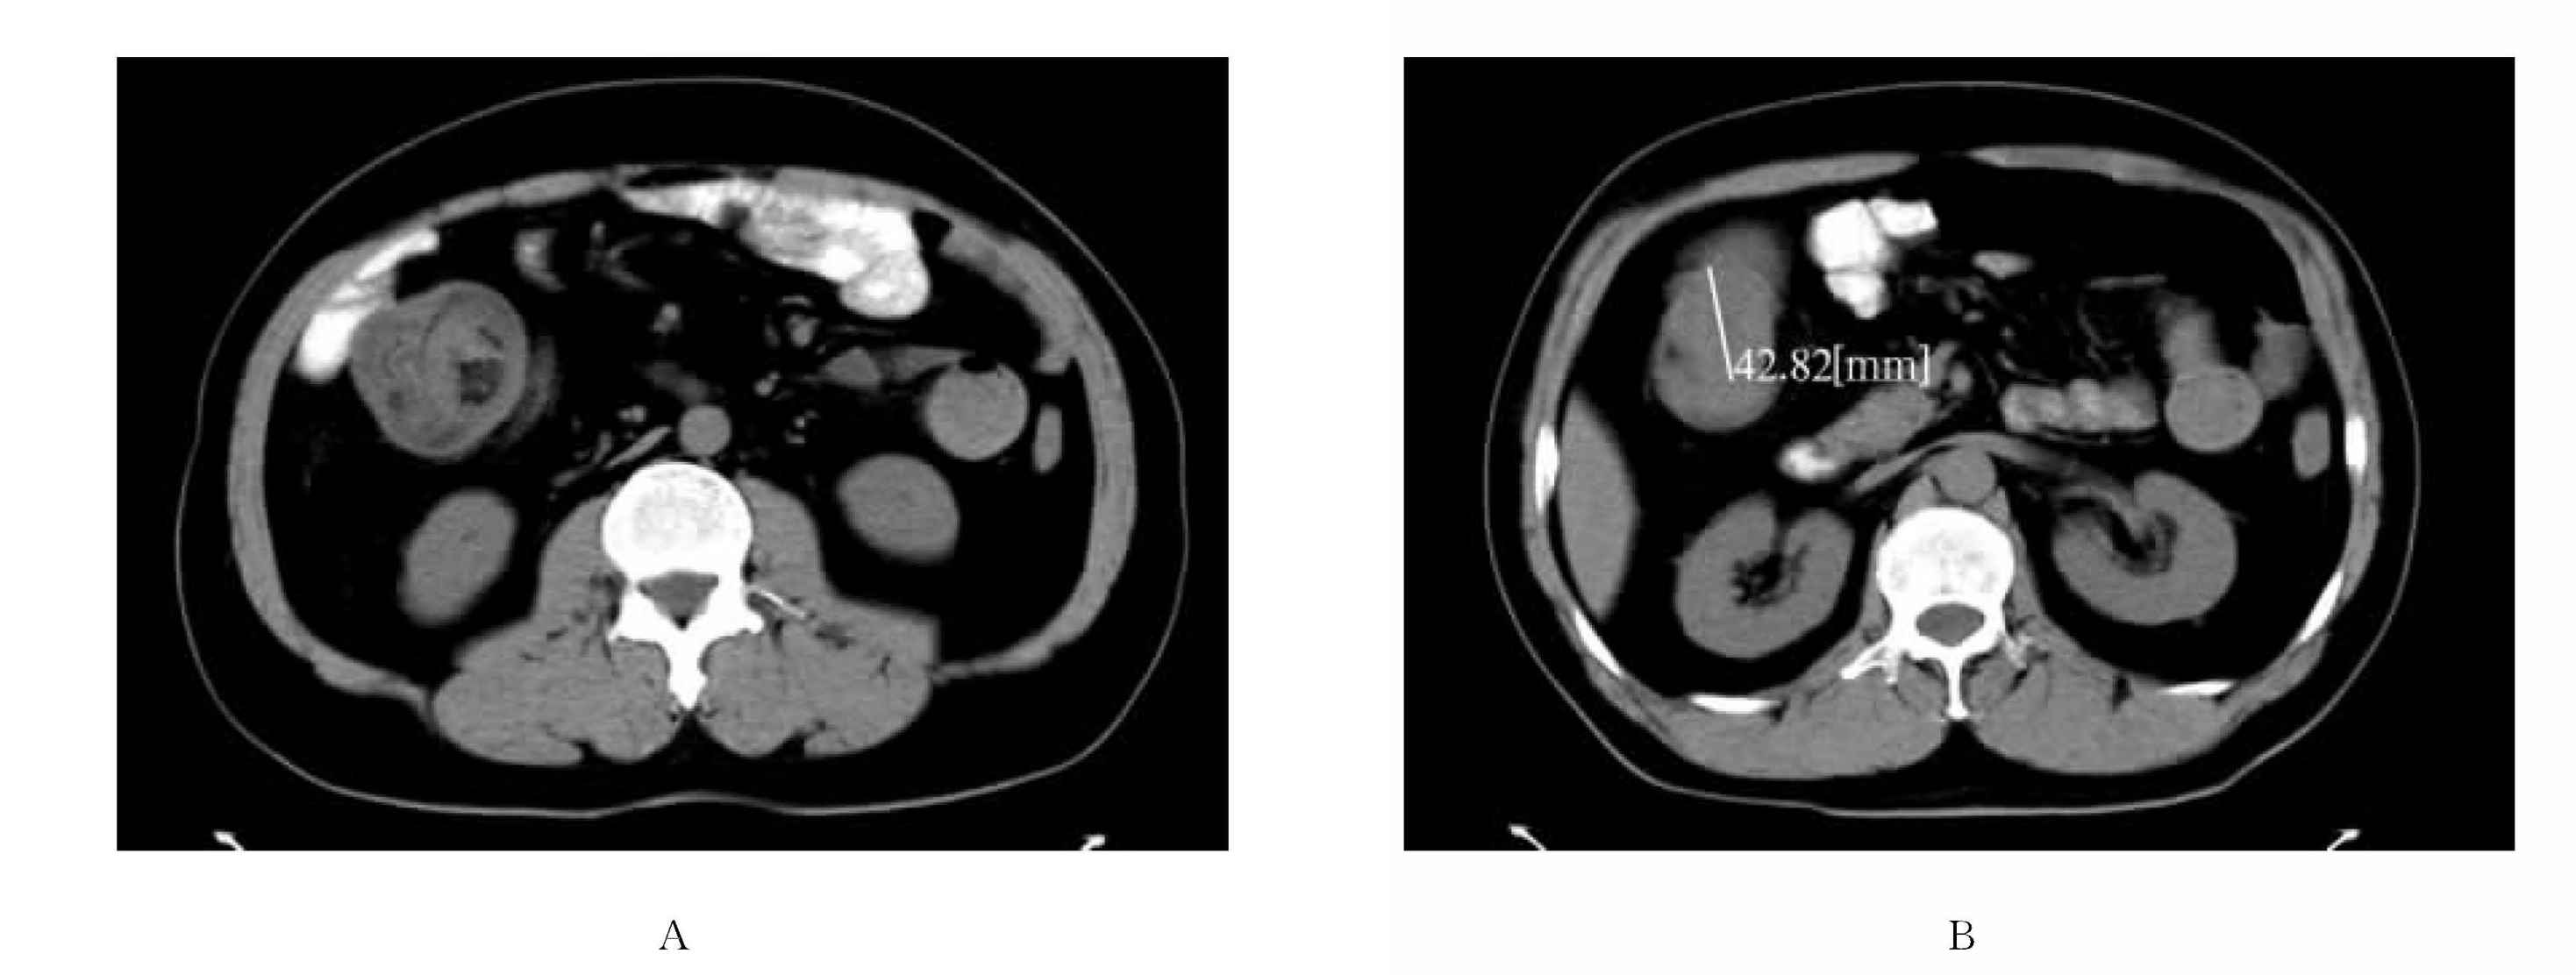
\includegraphics[width=.7\textwidth,height=\textheight,keepaspectratio]{./images/Image00369.jpg}
 \captionsetup{justification=centering}
 \caption{肠套叠\\{\small A、B为同一患者,为回肠末端息肉并发肠套叠。A示升结肠区套叠形成的“靶征”,B示套头部有4cm左右的软组织肿块}}
 \label{fig17-17}
  \end{figure} 

2.彗星尾征:即套叠近端肠系膜血管牵拉聚拢的征象。该征一般与肾形肿块相伴出现。国内有学者认为靶征见于各型肠套叠,而彗星征主要见于小肠型肠套叠。

3.其他征象:①附近扩张的肠管、散在的气-液平代表肠梗阻存在;②如果套入部脂肪层模糊,增厚的肠壁界限不清以致分层现象不清,受累的肠管被腹水包绕,提示可能出现穿孔;③肠壁内气体影代表套入部血运障碍。

4.原发病变的诊断:由于成人型肠套叠多为继发性,故应寻找原发病灶。CT应着重观察套头部,但除脂肪瘤可明确诊断外,其定性诊断仍有一定的难度。对于考虑恶性肿瘤者主要应鉴别是腺癌或淋巴瘤,肠系膜或腹膜后有较大的淋巴结可能有助于诊断淋巴瘤。

\protect\hypertarget{text00025.html}{}{}

